%--------------------------------------------------------------------%
% REV01: Fri 23 Jul 2021 20:08:29 WIB (RMS)
% Berkas utama templat LaTeX.
% author Petra Barus, Peb Ruswono Aryan
%--------------------------------------------------------------------%
% Berkas ini berisi struktur utama dokumen LaTeX yang akan dibuat.
%--------------------------------------------------------------------%
\documentclass[11pt, a4paper, onecolumn, oneside, final]{book}

%-------------------------------------------------------------------%
%
% Konfigurasi dokumen LaTeX untuk laporan tesis IF ITB
%
% @author Petra Novandi
%
%-------------------------------------------------------------------%
%
% Berkas asli berasal dari Steven Lolong
%
%-------------------------------------------------------------------%

% Ukuran kertas
\special{papersize=210mm,297mm}

% Setting margin
\usepackage[top=3cm,bottom=4cm,left=4cm,right=3cm]{geometry}

\usepackage{mathptmx}

% Judul bahasa Indonesia
\usepackage[bahasa]{babel}

% Format citation
%\usepackage[backend=bibtex,citestyle=authoryear]{biblatex}
\usepackage{natbib}

\usepackage[utf8]{inputenc}
\usepackage{csquotes}
\usepackage{graphicx}
\usepackage{titling}
\usepackage{blindtext}
\usepackage{sectsty}
\usepackage{chngcntr}
\usepackage{etoolbox}
\usepackage{hyperref}       % Package untuk link di daftar isi.
\usepackage{titlesec}       % Package Format judul
\usepackage{parskip}
%\usepackage{pgfgantt}
\usepackage{ragged2e}
\usepackage{libertine}
\usepackage{booktabs}
\usepackage{longtable}
\usepackage{array}
\usepackage{caption}
\usepackage{enumitem}
\usepackage{listings}
\usepackage{textcase}
\usepackage{setspace}
\usepackage{afterpage}
%\usepackage{tocloft}
\usepackage{amsmath,amsfonts}

\captionsetup[longtable]{skip=0.1em}

% Hypenation
%--------------------------------------------------------------------%
%
% Hypenation untuk Bahasa Indonesia
%
% @author Petra Barus
%
%--------------------------------------------------------------------%
%
% Secara otomatis LaTeX dapat langsung memenggal kata dalam dokumen,
% tapi sering kali terdapat kesalahan dalam pemenggalan kata. Untuk
% memperbaiki kesalahan pemenggalan kata tertentu, cara pemenggalan
% kata tersebut dapat ditambahkan pada dokumen ini. Pemenggalan
% dilakukan dengan menambahkan karakter '-' pada suku kata yang
% perlu dipisahkan.
%
% Contoh pemenggalan kata 'analisa' dilakukan dengan 'a-na-li-sa'
%
%--------------------------------------------------------------------%
% inhyph.tex 
% Version 1.3 19-SEP-1997
%
% Hyphenation patterns for bahasa indonesia (probably also usable
% for bahasa melayu)
%
% (c) Copyright 1996, 1997 J\"org Knappen and Terry Mart
% 
% This patterns are free software according to the GNU General Public 
% licence version 2, June 1991.
%
% Please read the GNU licence for details. If you don't receive a GNU
% licence with these patterns, you can obtain it from 
%
%                          Free Software Foundation, Inc.
%                          675 Mass Ave, Cambridge, MA 02139, USA
%
% If you make any changes to this file, please rename it so that it
% cannot be confused with the original one, and change the contact
% address for bug reports and suggestions.
%
% For bug reports, improvements, and suggestions, contact
%
% J\"org Knappen
% jk Unternehmensberatung
% Barbarossaring 43
% 55118 Mainz
%
% knappen@vkpmzd.kph.uni-mainz.de
%
% or:
% Terry Mart
%
% Institut fuer Kernphysik
% Universitaet Mainz
% 55099 Mainz
% Germany
%
% phone : +49 6131 395174
% fax   : +49 6131 395474
% email : mart@kph.uni-mainz.de
%
%*%*%*%*%*%*%*%*%*%*%*%*%*%*%*%*%*%*%*%*%*%*%*%*%*%*%*%*%*%*%*%*%*%*%*%*%*%*%*%*
%
% The patterns are best used with the following parameters
%
% \lefthyphenmin=2 \righthyphenmin=2 %
%
%*%*%*%*%*%*%*%*%*%*%*%*%*%*%*%*%*%*%*%*%*%*%*%*%*%*%*%*%*%*%*%*%*%*%*%*%*%*%*%*
%
% \patterns{%
% a1 e1 i1 o1 u1 % allow hyphens after vowels
% 2b1d 2b1j 2b1k 2b1n 2b1s 2b1t
% 2c1k 2c1n
% 2d1k 2d1n 2d1p 
% 2f1d 2f1k 2f1n 2f1t
% 2g1g 2g1k 2g1n
% 2h1k 2h1l 2h1m 2h1n 2h1w
% 2j1k 2j1n
% 2k1b 2k1k 2k1m 2k1n 2k1r 2k1s 2k1t
% 2l1b 2l1f 2l1g 2l1h 2l1k 2l1m 2l1n 2l1s 2l1t 2l1q
% 2m1b 2m1k 2m1l 2m1m 2m1n 2m1p 2m1r 2m1s
% 2n1c 2n1d 2n1f 2n1j 2n1k 2n1n 2n1p 2n1s 2n1t 2n1v
% 2p1k 2p1n 2p1p 2p1r 2p1t
% 2r1b 2r1c 2r1f 2r1g 2r1h 2r1j 2r1k 2r1l 2r1m 2r1n 2r1p 2r1r 2r1s 2r1t 2r1w 2r1y
% 2s1b 2s1k 2s1l 2s1m 2s1n 2s1p 2s1r 2s1s 2s1t 2s1w
% 2t1k 2t1l 2t1n 2t1t  
% 2w1t                 % two consonant groups to be hyphenated between
%                      % the consonants
% 2ng1g 2ng1h 2ng1k 2ng1n 2ng1s    % three consonant groups
% 2n3s2t % kon-stan-ta
% .be2r3 .te2r3 .me2ng3 .pe2r3 % prefixes
% 2ng. 2ny. % don't hyphenate -ng and -ny at the end of word
% i2o1n % in-ter-na-sio-nal
% a2ir % ber-air 
% 1ba1ga2i % se-ba-gai-ma-na
% 2b1an. 2c1an. 2d1an. 2f1an. 2g1an. 2h1an. 2j1an. 2k1an. 2l1an.
% 2m1an. 2ng1an. 2n1an. 2p1an. 2r1an. 2s1an. 2t1an. 2v1an. 2z1an. 
% 3an. % suffix -an
% .a2ta2u % atau-pan
% .ta3ng4an. .le3ng4an. .ja3ng4an. .ma3ng4an. .pa3ng4an. .ri3ng4an. 
% .de3ng4an. % Don't overload the exception list...
% }
% Exeptions to the above rules, specially words beginning in ber...
% and ter..
\hyphenation{be-ra-be be-ra-hi be-rak be-ran-da be-ran-dal be-rang
             be-ra-ngas-an be-rang-sang be-ra-ngus be-ra-ni
             be-ran-tak-an be-ran-tam be-ran-tas be-ra-pa be-ras
             be-ren-deng be-re-ngut be-re-rot be-res be-re-wok
             be-ri be-ri-ngas be-ri-sik be-ri-ta be-rok be-ron-dong
             be-ron-tak be-ru-du be-ruk be-run-tun
             peng-eks-por peng-im-por
             te-ra te-rang te-ras te-ra-si te-ra-tai te-ra-wang te-ra-weh
             te-ri-ak te-ri-gu te-rik te-ri-ma te-ri-pang te-ro-bos
             te-ro-bos-an te-ro-mol te-rom-pah te-rom-pet te-ro-pong
             te-ro-wong-an te-ru-buk te-ru-na te-rus te-ru-si}

\endinput

%\hyphenpenalty=5000
%\tolerance=1000
%\lefthyphenmin=2
%\righthyphenmin=2
\hyphenpenalty=10000
\tolerance=1
\lefthyphenmin=99
\righthyphenmin=99
\sloppy

% Line satu setengah spasi
\renewcommand{\baselinestretch}{1.5}

% Kode lebih kecil
\let\OldTexttt\texttt
\renewcommand{\texttt}[1]{\OldTexttt{\footnotesize{#1}}}

% Listing Code thingy
\lstset{frame=tb,
  breaklines=true,
  showstringspaces=false,
  columns=flexible,
  numbers=none,
  commentstyle=\color{dkgreen},
  stringstyle=\color{mauve},
  tabsize=3
}
\renewcommand{\lstlistingname}{Kode}
\newcommand{\listingsfont}{\ttfamily}

% Add comma between Author and Year
%\renewcommand*{\nameyeardelim}{\addcomma\space}

% Setting judul
\chapterfont{\centering \Large}
\titleformat{\chapter}[display]
  {\Large\centering\bfseries}
  {\chaptertitlename\ \thechapter}{0pt}
    {\Large\bfseries\uppercase}
\titlespacing*{\chapter}{0pt}{-25pt}{40pt}

% Setting nomor pada subbsubsubbab
\setcounter{secnumdepth}{4}

\titleformat{\paragraph}
{\normalfont\normalsize\bfseries}{\theparagraph}{1em}{}
\titlespacing*{\paragraph}
{0pt}{3.25ex plus 1ex minus .2ex}{1.5ex plus .2ex}

\titlespacing*{\section} {0pt}{2.5ex plus 1ex minus .2ex}{1.3ex plus .2ex}
\titlespacing*{\subsection} {0pt}{2.25ex plus 1ex minus .2ex}{0.5ex plus .2ex}

\makeatletter
\makeatother

% Counter untuk figure dan table.
\counterwithin{figure}{chapter}
\counterwithin{table}{chapter}

% For Gantt Chart
\newcounter{myWeekNum}
\stepcounter{myWeekNum}
%
\newcommand{\myWeek}{\themyWeekNum
    \stepcounter{myWeekNum}
    \ifnum\themyWeekNum=53
         \setcounter{myWeekNum}{1}
    \else\fi
}
%
\newcolumntype{L}[1]{>{\raggedright\let\newline\\\arraybackslash\hspace{0pt}}m{#1}}
\newcolumntype{C}[1]{>{\centering\let\newline\\\arraybackslash\hspace{0pt}}m{#1}}
\newcolumntype{R}[1]{>{\raggedleft\let\newline\\\arraybackslash\hspace{0pt}}m{#1}}

\makeatletter
\def\@chapter[#1]#2{\ifnum \c@secnumdepth >\m@ne
                         \refstepcounter{chapter}%
                         \typeout{\@chapapp\space\thechapter.}%
                         \addcontentsline{toc}{chapter}%
                                   {\protect{BAB \numberline{\thechapter}\texorpdfstring{\uppercase{#1}}{#1}}}%
                    \else
                      \addcontentsline{toc}{chapter}{\texorpdfstring{\uppercase{#1}}{#1}}%
                    \fi
                    \chaptermark{#1}%
                    \addtocontents{lof}{\protect\addvspace{10\p@}}%
                    \addtocontents{lot}{\protect\addvspace{10\p@}}%
                    \if@twocolumn
                      \@topnewpage[\@makechapterhead{#2}]%
                    \else
                      \@makechapterhead{#2}%
                      \@afterheading
                    \fi}
\makeatother

\makeatletter
\makeatother
%\bibliography{references}
\begin{document}

    %Basic configuration
    %\title{Pengembangan Aplikasi Pengumpulan Data Menggunakan \textit{Spreadsheet}}
    \title{Pengembangan Kakas Pengumpulan Data dalam Format \textit{Spreadsheet}}
    \date{}
    \author{
        Feryandi Nurdiantoro \\
        NIM : 13513042
    }   

    \frontmatter
    \clearpage
\pagestyle{empty}

\begin{center}
\smallskip

    \Large \bfseries \MakeUppercase{\thetitle}
    \vfill

    \Large Laporan Tugas Akhir
    \vfill

    \large Disusun sebagai syarat kelulusan tingkat sarjana
    \vfill

    \large Oleh

    \Large \theauthor

    \vfill
    \begin{figure}[h]
        \centering
            
\includegraphics[width=0.15\textwidth]{resources/cover-ganesha.jpg}
    \end{figure}
    \vfill

    \large
    \uppercase{
        Program Studi Teknik Informatika \\
        Sekolah Teknik Elektro dan Informatika \\
        Institut Teknologi Bandung
    }

    Agustus 2017
\end{center}

\clearpage

    \clearpage
\pagestyle{empty}

\begin{center}
\smallskip

    \Large \bfseries \MakeUppercase{\thetitle}
    \vfill

    \Large Laporan Tugas Akhir
    \vfill

    \large Oleh

    \Large \theauthor

    \large Program Studi Teknik Informatika \\
    \normalsize \normalfont
    Sekolah Teknik Elektro dan Informatika \\
    Institut Teknologi Bandung \\

    \vfill
    \normalsize \normalfont
    Telah disetujui dan disahkan sebagai Laporan Tugas Akhir \\ di Bandung, 23 Agustus 2017 \\
    Mengetahui,

    \vfill
    \setlength{\tabcolsep}{12pt}
    \begin{tabular}{c@{\hskip 0.5in}c}
        Pembimbing I, & Pembimbing II, \\
        & \\
        & \\
        & \\
        & \\
        \underline{Tricya Esterina Widagdo, ST., M.Sc.} & \underline{Yudistira Dwi Wardhana Asnar, Ph.D} \\
        NIP 197109071997022001 & NIP 198008272015041002 \\
    \end{tabular}

\end{center}
\clearpage

    \chapter*{Lembar Pernyataan}

Dengan ini saya menyatakan bahwa:

\begin{enumerate}

    \item Pengerjaan dan penulisan Laporan Tugas Akhir ini dilakukan tanpa menggunakan bantuan yang tidak dibenarkan.
    \item Segala bentuk kutipan dan acuan terhadap tulisan orang lain yang digunakan di dalam penyusunan laporan tugas akhir ini telah dituliskan dengan baik dan benar.
    \item Laporan Tugas Akhir ini belum pernah diajukan pada program pendidikan di perguruan tinggi mana pun.

\end{enumerate}

Jika terbukti melanggar hal-hal di atas, saya bersedia dikenakan sanksi sesuai dengan Peraturan Akademik dan Kemahasiswaan Institut Teknologi Bandung bagian Penegakan Norma Akademik dan Kemahasiswaan khususnya Pasal 2.1 dan Pasal 2.2.
\vspace{15mm}

Bandung, 4 Agustus 2017 \\
\vspace{20mm} \\
Feryandi Nurdiantoro \\
NIM 13513042 \\
\clearpage
    \pagestyle{plain}
    \clearpage
\chapter*{ABSTRAK}
\addcontentsline{toc}{chapter}{ABSTRAK}
\begin{center}
\MakeTextUppercase{\textbf{\large{\thetitle}}}

Oleh

\MakeTextUppercase{\theauthor}
\end{center}
\medskip
\begin{spacing}{1.0}
Pengumpulan data merupakan proses kerja yang sangat penting yang sering ditemui pada kehidupan sehari-hari. Pengumpulan data biasanya dilakukan menggunakan aplikasi \textit{spreadsheet}. Hal ini disebabkan oleh mudahnya penggunaan \textit{spreadsheet} sehingga banyak orang awam yang memilih menggunakan \textit{spreadsheet} dibandingkan basis data. Pengumpulan data menggunakan aplikasi \textit{spreadsheet} memiliki beberapa kelemahan seperti lemahnya validasi, terisolasinya data yang dikumpulkan, serta terdapat kemungkinan sulitnya berkolaborasi dalam pengumpulan data. Dari permasalahan tersebut, dibuat kakas pengumpulan data berbasis \textit{spreadsheet} yang diharapkan dapat memudahkan pengguna dalam melakukan pengumpulan data dan mengatasi permasalahan-permasalahan yang sering terjadi.

Kakas pengumpulan data ini diimplementasi sebagai fitur tambahan pada aplikasi EtherCalc sehingga permasalahan kolaborasi akan ditangani oleh aplikasi EtherCalc tersebut. Selanjutnya, pengguna dapat mendefinisikan \textit{metadata table} secara manual atau juga dilakukan secara otomatis oleh kakas menggunakan algoritma framefinder yang telah dibuat oleh penelitian lain. Dari \textit{metadata table} tersebut, pengguna dapat melakukan perubahan aturan-aturan validasi yang dibagi menjadi tiga tipe validasi yakni, tipe data, domain data, dan relasi antar data. Kakas akan menerjemahkan \textit{metadata table} yang dibuat serta mencocokkannya dengan data yang ada pada \textit{spreadsheet}, lalu memasukkan data tersebut ke dalam basis data relasional.

Pengujian dilakukan pada fitur-fitur yang diimplementasikan pada kakas. Pengujian dilakukan dengan menggunakan beberapa kasus yang dibuat dan diujikan kebenaran hasil data masukan menjadi data pada basis data.

Kata kunci: \textit{spreadsheet}, pengumpulan data, \textit{data quality}, \textit{data management}.
\end{spacing}

\clearpage
    %\clearpage
\chapter*{Abstract}
\addcontentsline{toc}{chapter}{Abstract}

The usage of spreadsheet in daily basis, usually used as a data collector. Spreadsheet is one of the easy to use software, so that many people prefer it as data management software than using a proper database management system. This could causing so many problems because the spreadsheet itself is not design to be a data collector. Some problem presisted as people use is as data collector, such as no data validation, isolation of data, and hard to collaborate. In order to solve those problem, this final year project want to create a spreadsheet software that could integrate with existing database and synchronize it with the data in the spreadsheet, could verify the data, and easy to collaborate.

This report will cover the analysis behind the software requirement in order to get the integrated software with the database. This will include data transformation with 4 steps, clustering, row identification, cell identification, and header-data assignment. This software is using two machine learning algorithm in order to do a proper transformation, the Hierarchical Clustering and Conditional Random Field. The training data set is from Statistical Abstract of the United States (SAUS) 2010 and some manual data gathering. The next step is validation, this software will cover 3 type of validation, such as data type, data domain, and data relation. Those algorithm build on top of an open source spreadsheet software called EtherCalc which already could do online collaboration.

Keyword: spreadsheet, data collector, data quality, data management.
\clearpage
    \chapter*{Kata Pengantar}
\addcontentsline{toc}{chapter}{KATA PENGANTAR}

Puji syukur saya panjatkan kehadirat Tuhan Yang Maha Esa, karena degan kelimpahan rahmat dan kemurahan hati-Nya penulis dapat menyelesaikan Tugas Akhir yang berjudul "\thetitle". 

Dalam penyusunan Tugas Akhir ini penulis banyak mendapatkan masukan, kritik, dorongan, bantuan, bimbingan, serta dukungan baik secara fisik maupun moral dari berbagai pihak yang merupakan pengalaman yang berharga yang tidak dapat diukur secara materi dan dapat menjadi pembelajaran yang berharga dikemudian hari. Oleh karena itu dengan segala hormat dan kerendahan hati perkenankanlah penulis mengucapkan terima kasih kepada:

\begin{enumerate}
	\item Bapak Yudistira Dwi Wardhana Asnar, Ph.D dan Ibu Tricya Esterina Widagdo, ST., M.Sc. selaku pembimbing yang senantiasa memberikan arahan dan masukan selama pengerjaan Tugas Akhir.
	\item Bapak Adi Mulyanto, ST., MT. selaku dosen penguji yang atas saran dan masukkannya membuat Tugas Akhir ini menjadi lebih baik.
	\item Kedua orang tua penulis. Terima kasih atas dukungan baik secara moral dan material sehingga penulis dapat melaksanakan Tugas Akhir ini hingga selesai dengan baik.
	\item Ibu Dr. Fazat Nur Azizah ST, M.Sc. selaku dosen Tugas Akhir yang telah mendukung saya dan memberikan arahan dalam penyelesaian dan pengerjaan Tugas Akhir ini.
	\item Ibu Dr. Eng. Ayu Purwarianti, ST., MT. selaku dosen mentor Imagine Cup yang ikut membantu dan memberikan dukungan agar penulis dapat menyelesaikan pengerjaan Tugas Akhir.
	\item Bapak Dr.techn. Saiful Akbar ST, MT. dan Bapak Achmad Imam Kistijantoro, ST, M.Sc, Ph.D selaku Ketua Program Studi dari Teknik Informatika dan Sistem dan Teknologi Informasi yang ikut mendukung penulis dalam menyelesaikan Tugas Akhir ini.
	\item Seluruh dosen, karyawan dan civitas program studi Teknik Informatika, Institut Teknologi Bandung.
	\item Rekan-rekan yang telah penulis minta bantuan dalam penyelesaian administrasi Tugas Akhir ini disaat penulis berhalangan terutama Muhamad Visat Sutarno dan Fiqie Ulya Sidiastahta
	\item Rekan-rekan laboratorium basis data yang saling mendukung dalam menyelesaikan Tugas Akhir ini pada khususnya Vanya Deasy Safrina, Albert Tri Adrian, Marco Orlando, Fiqie Ulya Sidiastahta, dan Wilhelmus Andrian.
	\item Rekan-rekan seperjuangan Teknik Informatika yang menamakan dirinya Happy Anti Wacana yang selalu mendukung penulis untuk mengerjakan Tugas Akhir.
	\item Rekan-rekan dari Binary 2013 dan HMIF yang telah memberikan dukungan dan bantuan dalam pengerjaan Tugas Akhir.
	\item Pihak-pihak lain yang tidak dapat disebutkan satu-persatu.
\end{enumerate}

Penulis menyadari bahwa Tugas Akhir ini masih jauh dari sempurna serta memiliki banyak kekurangan. Oleh karena itu, penulis sangat terbuka dalam menerima kritik dan saran yang membangun untuk Tugas Akhir ini. Semoga Tugas Akhir ini dapat bermanfaat bagi pembaca.

\begin{flushright}
Bandung, Agustus 2017 \\
\vspace{25mm}
Penulis
\end{flushright}

    \titleformat*{\section}{\centering\bfseries\Large\MakeUpperCase}
    \tableofcontents
    \addcontentsline{toc}{chapter}{DAFTAR ISI}
    % \afterpage{\null\newpage}
    % \addcontentsline{toc}{chapter}{DAFTAR LAMPIRAN}
    {%
        \let\oldnumberline\numberline%
        \renewcommand{\numberline}{\figurename~\oldnumberline}%
        \listoffigures%
    }
    \addcontentsline{toc}{chapter}{DAFTAR GAMBAR}
    {%
        \let\oldnumberline\numberline%
        \renewcommand{\numberline}{\tablename~\oldnumberline}%
        \listoftables%
    }
    \addcontentsline{toc}{chapter}{DAFTAR TABEL}

    %----------------------------------------------------------------%
    % Konfigurasi Bab
    %----------------------------------------------------------------%
    \renewcommand{\chaptername}{BAB}
    \renewcommand{\thechapter}{\Roman{chapter}}
    %----------------------------------------------------------------%

    \titleformat*{\section}{\bfseries\large}
    \mainmatter
    %----------------------------------------------------------------%
    % Dafter Bab
    % Untuk menambahkan daftar bab, buat berkas bab misalnya `chapter-6` di direktori `chapters`, dan masukkan ke sini.
    %----------------------------------------------------------------%
    \chapter{Pendahuluan}

Pada bab ini akan dibahas mengenai gambaran dasar dari pelaksanaan Tugas Akhir dalam bentuk penjelasan latar belakang yang mendasari pemilihan topik. Dari latar belakang tersebut, akan diurai kembali menjadi rumusan masalah, tujuan, batasan masalah, serta metodologi yang digunakan untuk keperluan Tugas Akhir ini.

\section{Latar Belakang}

Aplikasi \textit{spreadsheet} merupakan aplikasi yang mudah ditemui dan wajar digunakan oleh banyak orang, baik secara personal maupun dalam sebuah organisasi komersial \citep{Chan1996}. Pada tahun 1979, aplikasi \textit{spreadsheet} pertama dibuat dengan nama VisiCalc. Pengguna komputer pada saat itu dimanjakan dengan kapabilitas dan fleksibilitas aplikasi yang dapat melakukan operasi sederhana tanpa harus menggunakan komputer \textit{mainframe}. Dengan semakin berkembangnya daya komputasi, saat ini telah banyak sekali muncul aplikasi \textit{spreadsheet} baru dan penggunaannya juga semakin beragam.

\textit{Spreadsheet} memiliki beberapa keunggulan dibandingkan dengan aplikasi pengolahan data jenis lain. Keunggulan yang paling terlihat adalah banyak orang yang mengetahui cara penggunaan aplikasi jenis \textit{spreadsheet} dan terbiasa dalam menggunakannya. Di samping itu, \textit{spreadsheet} memiliki banyak fitur dan kemampuan yang jarang diketahui orang awam jika digunakan dengan benar. Dengan keunggulan ini, \textit{spreadsheet} sering kali dijadikan pilihan utama dalam pengolahan dan pengumpulan data. Beberapa orang mungkin menganggap, penggunaan \textit{spreadsheet} adalah personal sehingga tidak membutuhkan tim atau bantuan orang lain dalam pembuatan suatu \textit{spreadsheet}. Hal ini tidak dapat dibenarkan, karena jika melihat kasus penggunaannya pada organisasi bisnis yang besar, \textit{spreadsheet} yang dihasilkan sangatlah kompleks dan besar dengan pengembangan yang membutuhkan banyak orang \citep{Panko1998}. 

Penggunaan \textit{spreadsheet} yang dapat ditemui pada perusahaan atau instansi adalah sebagai media pengumpulan data. Data yang dikumpulkan biasanya dalam bentuk \textit{data frame} yakni \textit{spreadsheet} yang mempunyai dua struktur utama yaitu bagian \textit{value} atau data dan bagian \textit{atribute} atau label \citep{Chen2013}. Data yang telah dikumpulkan biasanya akan disebarkan kepada pihak-pihak yang membutuhkan atau disimpan sebagai arsip data yang akan digunakan kembali pada saat dibutuhkan.

Sebagai media pengumpulan data, \textit{spreadsheet} memiliki permasalahan penyimpanan data. Hal tersebut penting untuk diperhatikan jika data yang dikumpulkan mungkin tidak hanya akan ditampilkan dalam bentuk \textit{spreadsheet} namun juga dapat digunakan oleh aplikasi lain. Permasalahan lain yang mungkin muncul adalah kompleksitas dan besarnya ukuran data pada \textit{spreadsheet} yang membuat penggunaan \textit{spreadsheet} pada sebuah bisnis sangatlah rentan akan kesalahan. Sebuah kesalahan kecil dapat berakibat fatal dan memberikan kerugian seperti kehilangan pendapatan, kesalahan pemberian harga, penipuan, dan kegagalan sistem akibat ketergantungan berlebih antar \textit{spreadsheet} \citep{EUSPRIGAbout}. Telah banyak bukti dan penelitian yang menunjukan bahwa kesalahan pada \textit{spreadsheet} sangat mudah ditemui. %Bahkan pada \textit{spreadsheet} yang dibuat dengan sangat hati-hati, masih dapat ditemui sekitar 1 persen atau lebih kesalahan pada formula yang dibuat \citep{Panko1998}.
Contoh kesalahan yang dapat terjadi adalah kesalahan tipe data, kesalahan masukan, tidak divalidasinya data masukan, serta permasalahan \textit{single version of truth} dimana bisa terdapat dua atau lebih versi dari data yang sama.

% Tingginya angka kesalahan yang dapat terjadi pada suatu \textit{spreadsheet} merupakan hal yang sangat krusial terutama di dalam bisnis. Metode pencegahan harus dapat dilakukan untuk dapat mengurangi angka kesalahan ini. Beberapa organisasi dapat menerapkan pencegahan dengan cara melakukan tahap-tahap metodologi yakni dengan pembuatan desain awal, melakukan metode \textit{best practice} yang tersedia dan sesuai dengan situasi yang dihadapi, menerapkan \textit{policy} khusus pada saat pembuatan \textit{spreadsheet}, melakukan \textit{testing}, serta pembuatan dokumentasi \citep{EUSPRIGBestPractice}. Namun, metodologi tersebut masih sangat rentan oleh kesalahan manusia karena perangkat lunak yang digunakan tetap tidak diubah didalam menjalankan metodologi tersebut.

Untuk dapat mengurangi kesalahan-kesalahan yang sering terjadi pada \textit{spreadsheet} secara lebih mendasar, dibutuhkan bantuan perangkat lunak untuk dapat melakukan kontrol terhadap masukan pengguna, melakukan validasi, serta dapat melakukan penyimpanan data yang telah dikumpulkan. Pada tugas akhir ini akan difokuskan pada pengembangan sebuah aplikasi pengumpulan data berbentuk \textit{spreadsheet} yang dapat membantu pengguna mengurangi terjadinya masalah-masalah yang telah disebutkan sebelumnya.

\section{Rumusan Masalah}\label{RumusanMasalah}

Seperti yang telah dijelaskan pada latar belakang, salah satu penggunaan aplikasi \textit{spreadsheet} adalah sebagai media pengumpulan data. Beberapa permasalahan yang muncul dalam pengumpulan data adalah kolaborasi, validasi, dan penyimpanan data. Pengumpulan data dapat dilakukan oleh banyak orang secara bersama-sama sehingga dapat menyebabkan konflik pada data masukan. Konflik ini bisa terjadi karena terdapat lebih dari satu versi file yang diubah secara bersama-sama. Di samping itu, data yang dimasukkan biasanya tidak melalui proses validasi sehingga dapat menyalahi domain data yang seharusnya. Setelah data dikumpulkan ke dalam bentuk \textit{spreadsheet}, diperlukan media penyimpanan data sehingga data tidak terisolasi. Contoh dari media penyimpanan tersebut adalah menggunakan basis data. 

Hal-hal tersebut merupakan beberapa masalah utama yang cukup penting untuk diselesaikan terutama dalam penggunaannya pada bisnis dan komersial sehingga akan dibentuk sebuah kakas yang membantu pengumpulan data pada format \textit{spreadsheet}. Dalam rangka pembangunan kakas, terdapat beberapa permasalahan yang menjadi perhatian pada tugas akhir ini, yaitu:

\begin{enumerate}
    %\item Bagaimana cara menangani konflik yang terjadi pada saat kolaborasi?
    \item Bagaimana cara melakukan validasi terhadap data masukan?
    \item Bagaimana cara data pada \textit{spreadsheet} dapat disimpan pada basis data?
    \item Bagaimana cara melakukan penyimpanan data yang telah dibuat?
    \item Bagaimana proposal perubahan alur kerja yang terjadi akibat penggunaan kakas yang dibuat?
\end{enumerate}

\section{Tujuan}

Tujuan yang ingin dicapai dalam Tugas Akhir ini adalah mengembangkan perangkat lunak pengumpulan data berbentuk \textit{spreadsheet} yang dapat mengubah data dalam format \textit{spreadsheet} menjadi data relasional serta melakukan validasi pada data masukan. Dengan adanya perangkat lunak ini diharapkan dapat dilakukan pengumpulan data yang disertai validasi data masukan.

\section{Batasan Masalah}

Dalam pengerjaan Tugas Akhir ini, terdapat beberapa batasan-batasan yang perlu diperhatikan. Batasan tersebut ditujukan untuk memperjelas dan memfokuskan objek penelitian dan pengembangan tugas akhir. Batasan-batasan masalah pengerjaan tugas akhir adalah sebagai berikut,

\begin{enumerate}
    %\item Fitur kolaborasi pada \textit{spreadsheet} bukan fokus utama, fitur akan diambil dari aplikasi \textit{spreadsheet} yang telah ada.
    %\item Fokus data masukan pada Tugas Akhir ini berupa data mentah yang belum direkapitulasi.
    \item Kakas hanya dapat berjalan pada aplikasi EtherCalc.
    \item Jenis \textit{spreadsheet} yang ditangani adalah \textit{data frame} dan relasi.
    \item Data disimpan dalam bentuk basis data relasional.
    \item Basis data yang didukung untuk digunakan dalam penyimpanan data hanya MySQL.
    \item Struktur basis data dan tingkat normalisasi yang terbentuk merupakan tanggung jawab pengguna dan tidak ditangani oleh kakas.
    \item Kakas hanya mendukung penggunaan satu \textit{sheet} dalam satu \textit{spreadsheet}.
    \item Validasi yang dilakukan hanya validasi tipe, domain, dan relasi data.
    \item Validasi tipe hanya mencakup tipe \textit{integer}, \textit{double}, \textit{string}, dan \textit{boolean}.
    \item Validasi domain hanya mencakup aturan \textit{range}, lebih besar, lebih kecil, sama dengan, dan nilai diskrit. Atribut hanya dapat menerima satu aturan validasi domain.
\end{enumerate}

\section{Metodologi}

Metodologi yang digunakan dalam pengerjaan Tugas Akhir ini yakni:
\begin{enumerate}
    \item Studi Literatur \\
    Pengerjaan tugas akhir diawali dengan mencari dan mempelajari referensi berupa jurnal ilmiah dan aplikasi-aplikasi yang telah ada sebelumnya yang dapat membantu pengembangan kakas yang dibuat pada tugas akhir ini. Literatur yang dicari dan dipelajari berkaitan dengan topik tugas akhir yaitu mengenai \textit{spreadsheet}, penggunaannya pada bisnis, kesalahan yang sering dilakukan dalam pembuatan, teknik pendeteksian data yang ada pada \textit{spreadsheet}, serta hal-hal lain yang masih berkaitan dengan topik tugas akhir ini. 
    
    \item Analisis Masalah \\
    Pada tahap ini dilakukan analisis permasalahan yang berkaitan dengan topik yang diangkat pada tugas akhir ini. Diantaranya adalah memecah permasalahan menjadi aplikasi \textit{spreadsheet} yang dikembangkan, penanganan konflik saat berkolaborasi, jenis \textit{spreadsheet} yang ditangani, metode interaksi pengguna, penentuan bagian data dan label, representasi tabel, validasi data, penyimpanan data, interaksi antar \textit{spreadsheet}, dan proposal perubahan alur kerja.

    \item Perancangan Solusi \\
    Pada tahap ini dilakukan perancangan solusi yang dapat menyelesaikan masalah-masalah yang telah dijelaskan pada bagian analisis masalah. Bagian perancangan ini juga menjelaskan arsitektur yang digunakan untuk membangun perangkat lunak berdasarkan spesifikasi dan metode yang digunakan.

    \item Implementasi \\
    Pada tahap ini dilakukan pembangunan kakas sesuai dengan kebutuhan dan spesifikasi dari hasil analisis masalah serta rancangan solusi yang diajukan.

    \item Pengujian dan Analisis Hasil \\
    Pada tahap ini dilakukan pengujian dengan menggunakan data set uji yang sesuai dengan batasan masalah ke dalam kakas yang diimplementasikan. Selanjutnya dilakukan analisis hasil pengujian dan penarikan kesimpulan.

\end{enumerate}

\section{Sistematika Pembahasan}

Penulisan tugas akhir ini terdiri dari 5 bab, yaitu: BAB I Pendahuluan, BAB II Tinjauan Pustaka, BAB III Analisis dan Perancangan, BAB IV Rancangan, Implementasi, dan Pengujian, dan BAB V Penutup. 

Bab satu membahas mengenai latar belakang permasalahan, rumusan masalah, tujuan, batasan masalah, metodologi serta sistematika pembahasan yang digunakan. Bab ini juga menjelaskan secara umum isi dari tugas besar serta gambaran dasar dari pelaksanaan tugas akhir.

Bab dua menjelaskan mengenai dasar teori yang digunakan di dalam menyelesaikan permasalahan yang diangkat. Teori yang digunakan berasal dari literatur dan referensi yang berhubungan dengan permasalahan yang diangkat seperti hal-hal yang berkaitan dengan \textit{spreadsheet}, penggunaannya pada bisnis, masalah yang sering terjadi dalam pembuatan, metode \textit{quality control} yang dapat dilakukan untuk mencegah kesalahan, serta metode pendeteksian bagian label dan data yang pernah dibuat pada penelitian lain. Dasar teori ini menjadi dasar analisis dan rancangan solusi pada bab selanjutnya.

Bab tiga memaparkan analisa kebutuhan dan permasalahan yang dipilih yakni tingginya tingkat kesalahan yang terjadi pada \textit{spreadsheet}. Dari hasil analisa yang dilakukan, di dapatkan bentuk solusi umum yang dapat digunakan untuk mengatasi permasalahan tersebut. Selanjutnya solusi umum tersebut dibuat rancangan dan arsitekturnya agar dapat diimplementasikan.

Bab empat memperlihatkan rancangan perangkat lunak yang dibuat serta hasil implementasinya. Pada akhir bab akan ditunjukkan hasil pengujian yang dilakukan kepada kakas yang dibuat dan pembahasan dari pengujian tersebut. Pengujian dilakukan untuk mengetahui keberhasilan kakas yang dibuat untuk menyelesaikan permasalahan yang di definisikan pada rumusan masalah.

Bab lima berisikan kesimpulan terhadap hasil implementasi dan solusi yang dipaparkan untuk menyelesaikan permasalahan. Di samping itu, terdapat bagian saran yang memaparkan saran pengembangan dan perbaikan yang dapat dilakukan untuk memperkaya fitur dan menyelesaikan permasalahan yang lebih luas.

% \section{Jadwal Pelaksanaan}
% \newsavebox\mybox
% \begin{lrbox}{\mybox}
%     \begin{ganttchart}[
%     vgrid={*{6}{draw=none}, dotted},
%     x unit=.05cm,
%     y unit title=.6cm,
%     y unit chart=.6cm,
%     time slot format=isodate,
%     time slot format/start date=2016-09-01]{2016-09-01}{2017-04-30}
%     \ganttset{bar height=.6}
%     \gantttitlecalendar{year, month} \\
%     \ganttbar[bar/.append style={fill=blue}]{Tahap 1}{2016-09-01}{2016-11-30}\\
%     \ganttbar[bar/.append style={fill=blue}]{Tahap 2}{2016-10-01}{2016-11-15}\\
%     \ganttbar[bar/.append style={fill=blue}]{Tahap 3}{2016-11-01}{2016-12-15}\\
%     \ganttbar[bar/.append style={fill=blue}]{Tahap 4}{2016-12-15}{2017-03-01}\\
%     \ganttbar[bar/.append style={fill=blue}]{Tahap 5}{2017-02-01}{2017-04-30}
%     \end{ganttchart}
% \end{lrbox}

% Pengerjaan tugas akhir ini direncanakan mulai pada September 2016 sampai April 2016. Pelaksanaan tugas akhir ini dibagi menjadi 5 tahap yang dapat dipetakan kepada metodologi pengerjaan sebagai berikut,
% \begin{enumerate}
%     \item Tahap 1: Studi Literatur
%     \item Tahap 2: Analisis Masalah
%     \item Tahap 3: Perancangan Solusi
%     \item Tahap 4: Implementasi
%     \item Tahap 5: Pengujian dan Analisis Hasil
% \end{enumerate}
% Jadwal pelaksanaan tugas akhir berdasarkan metodologi pengerjaan tugas akhir dapat dilihat pada Tabel \ref{Gantt-Chart} dibawah ini.
% \begin{table}[htb]
% \centering
% \caption{Gantt Chart jadwal pelaksanaan tugas akhir}
% \label{Gantt-Chart}
% \tikz{
%   \node[inner sep=0pt,outer sep=0pt] (gantt)
%   {\begin{tabular}{c}
%     \toprule
%     \resizebox{\textwidth}{!}{\usebox\mybox} \\
%     \bottomrule
%    \end{tabular}%
%    };
% }   
% \end{table}
    \chapter{Studi Literatur}

Pada bab ini akan dideskripsikan kajian literatur yang terkait dengan persoalan Tugas Akhir. Studi literatur ini akan dijadikan dasar di dalam melakukan penyelesaian persoalan yang telah didefinisikan.

\section{\textit{Spreadsheet}}
Bagian ini akan membahas mengenai definisi umum \textit{spreadsheet} serta teknologi yang sering digunakan di dalam membuat \textit{spreadsheet}. Dengan adanya definisi umum ini diharapkan dapat menyamakan persepsi mengenai \textit{spreadsheet} yang dimaksud pada Tugas Akhir ini. Teknologi yang dijelaskan pada bagian ini merupakan teknologi yang memungkinkan untuk dijadikan dasar pengembangan perangkat lunak pada Tugas Akhir ini.

\subsection{Definisi Umum}
Secara harafiah, \textit{spreadsheet} adalah suatu perangkat lunak yang dapat melakukan kalkulasi terhadap angka serta mengorganisir informasi yang ada di dalamnya berdasarkan kolom dan baris \citep{meriamwebster-spreadsheet}. Konsep dasar pada aplikasi \textit{spreadsheet} modern adalah sebuah aplikasi yang berupa sekumpulan sel terdiri dari baris dan kolom yang disebut \textit{sheet} yang dapat digambarkan sebagai matriks yang besar \citep{Ronen1989}.

Sel-sel pada \textit{spreadsheet} dapat diisi data berupa data mentah maupun formula. Data mentah dapat berupa angka, teks, tanggal, dan nilai mata uang. Formula merupakan perintah yang dapat dimengerti komputer untuk menghitung dan memanipulasi data pada sel. Data hasil pengolahan dan masukan pada \textit{spreadsheet} ditampilkan dalam bentuk sel yang namanya terdiri dari nama kolom dan nilai baris (Contoh: A1 untuk kolom pertama dan baris pertama). Di samping itu, sel tersebut juga dapat memiliki \textit{properties} berupa \textit{value} yang diisikan, format sel, serta format data yang digunakan.

\subsection{Teknologi \textit{Spreadsheet}} \label{TeknologiSpreadsheet}
Perkembangan teknologi \textit{spreadsheet} digital modern dimulai pada tahun 1978, saat Bricklin mengembangkan \textit{working prototype} dari konsep dasar \textit{spreadsheet} menggunakan Integer BASIC. Pada tahun yang sama, Frankston dan Fylstra bergabung dan membentuk sebuah perangkat lunak bernama VisiCalc (Visible Calculator) yang merupakan sebuah perangkat lunak \textit{spreadsheet} pertama yang bekerja dengan baik dan sukses dipasaran. Setelah keberhasilan VisiCalc, mulai muncul aplikasi serupa yang semakin baik salah satunya adalah Lotus. Dengan berkembangnya daya komputasi dan munculnya konsep \textit{graphical user interface}, Microsoft mengembangkan Microsoft Excel yang merupakan \textit{spreadsheet} pertama yang menggunakan antarmuka grafis dan menggunakan \textit{mouse} sebagai alat kontrol \citep{power2004brief}.

Saat ini, perangkat lunak berupa \textit{spreadsheet} sangat banyak variasi dan tipenya. Perangkat lunak \textit{spreadsheet} ini dapat dibagi berdasarkan konektivitasnya yakni \textit{offline spreadsheet} dan \textit{online spreadsheet}. Selain itu, perangkat lunak \textit{spreadsheet} dapat juga dibagi berdasarkan keterbukaan dari \textit{source code} yakni \textit{open source} dan \textit{closed source}. Bagian ini akan membahas masing-masing perangkat lunak tersebut secara umum.

    \subsubsection{Microsoft Excel}
    Microsoft Excel adalah perangkat lunak yang dikembangkan oleh Microsoft yang menyediakan fitur dasar dari \textit{spreadsheet} serta dengan fitur-fitur lainnya yang selalu ditambahkan pada setiap iterasi pengembangan Excel. Microsoft Excel dapat dimiliki oleh pengguna melalui pembelian paket Microsoft Office yang berisikan produk esensial Microsoft lainnya \citep{MSExcelProduct}. 

    Sejak Microsoft Excel 2007, Microsoft menggunakan format Office Open XML (OOXML) sebagai format penyimpanan \citep{MSExcelSupport}. Office Open XML dikembangkan oleh Microsoft mulai dari tahun 2000 dengan diimplementasinya dukungan XML pada Microsoft Office 2000. Pada awal penggunaan aplikasi \textit{office}, terdapat permasalahan \textit{data interoperability} antar mesin dan sulitnya manipulasi data. Office Open XML diharapkan dapat menyelesaikan permasalahan ini dengan membentuk standar yang dapat diimplementasi berbagai aplikasi \textit{office} \citep{OOXMLFormat}.

    \subsubsection{LibreOffice Calc}
    LibreOffice adalah perangkat lunak yang dikembangkan oleh komunitas dan proyek dari organisasi non-profit bernama The Document Foundation. LibreOffice adalah perangkat lunak yang gratis dan \textit{open source} yang awalnya didasarkan pada perangkat lunak serupa yakni OpenOffice.org dan merupakan pengembangan lanjutan dari OpenOffice yang paling aktif. Hampir serupa dengan Microsoft Office, LibreOffice memberikan 6 perangkat lunak yang ada di dalamnya yakni: Writer (pemrosesan teks), Calc (\textit{spreadsheet}), Impress (presentasi), Draw (grafik dan vektor), Base (basisdata), dan Math (editor formula) \citep{LibreOffice}. 

    LibreOffice Calc memiliki berbagai kemampuan yang dimiliki oleh kebanyakan \textit{spreadsheet}. Di dalam melakukan penyimpanan file, Calc menggunakan format OpenDocument. Format OpenDocument dikembangkan oleh Organization for the Advancement of Structured Information Standards (OASIS) yang bertujuan untuk membentuk \textit{open standard} bagi \textit{office document} \citep{OpenDocument}. 

    \subsubsection{EtherCalc} \label{AboutEtherCalc}
    EtherCalc merupakan perangkat lunak \textit{spreadsheet online} yang \textit{open-source} yang dikembangkan oleh Audrey Tang. EtherCalc merupakan pengembangan yang didasarkan dari perangkat lunak serupa yakni WikiCalc dan SocialCalc. WikiCalc merupakan aplikasi \textit{spreadsheet} yang mengandalkan komputasi server untuk dapat berkolaborasi, sedangkan SocialCalc merupakan aplikasi \textit{spreadsheet} yang menggunakan kemampuan javascript untuk melakukan komputasi pada \textit{client-side}. EtherCalc dikembangkan di atas Node.js dan menggunakan javascript sebagai alat komputasi. 

    Arsitektur aplikasi EtherCalc berjalan di atas aplikasi SocialCalc. Fungsi-fungsi dasar yang ada pada \textit{spreadsheet} hampir seluruhnya menggunakan implementasi SocialCalc. EtherCalc menjadikan aplikasi dalam bentuk Node.js, memiliki fitur kolaborasi yang lebih baik, dan beberapa fitur lain seperti pembuatan grafik data. Pada Gambar \ref{ModulEtherCalc} dapat dilihat interaksi antar modul yang terjadi pada EtherCalc.

    \begin{figure}[htb]
        \centering
        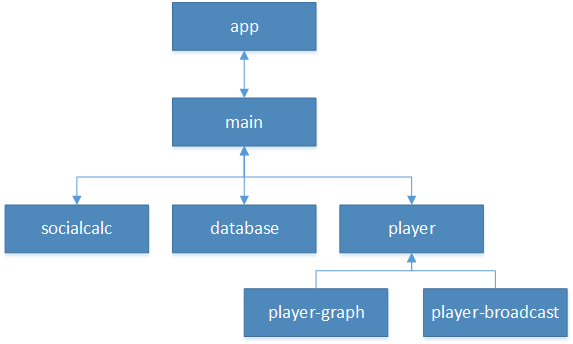
\includegraphics[width=0.6\textwidth]{resources/chapter-2-module-ethercalc.png}
        \caption{Arsitektur Module pada EtherCalc}
        \label{ModulEtherCalc}
    \end{figure}  

    Modul-modul tersebut memiliki tugas antara lain sebagai berikut:
    \begin{enumerate}
        \item Modul App \\
        Merupakan modul utama yang berisikan variabel konstanta dan pengaturan yang dibutuhkan oleh aplikasi.
        \item Modul Main \\
        Modul ini bertugas sebagai modul pertama yang menerima perintah dari pengguna dan mengatur API yang ada pada aplikasi. Modul ini mengatur hubungan antara modul player, modul database, dan modul socialcalc.
        \item Modul Socialcalc \\
        Merupakan modul yang bertugas merepresentasikan \textit{spreadsheet} pada aplikasi. Di dalam modul ini terdapat fungsi-fungsi yang dapat digunakan untuk memanipulasi sel-sel yang ada pada \textit{spreadsheet}.
        \item Modul Database \\
        Modul ini bertugas untuk memanipulasi basis data redis yang menyimpan perubahan-perubahan yang terjadi pada \textit{spreadsheet}.
        \item Modul Player \\
        Modul ini memiliki tugas untuk menjembatani \textit{front-end} dan \textit{back-end} dari aplikasi.
    \end{enumerate}

    Perangkat lunak hanya akan melakukan panggilan ke \textit{server} saat melakukan suatu aksi dan \textit{server} yang bertugas untuk menyimpan kumpulan aksi tersebut agar pengguna lain yang ikut berkolaborasi dapat melihat \textit{spreadsheet} yang sama satu dengan yang lain \citep{EtherCalc}. Gambar \ref{IlustrasiEtherCalc} merupakan gambaran umum cara kerja EtherCalc dalam berkolaborasi.

    \begin{figure}[htb]
        \centering
        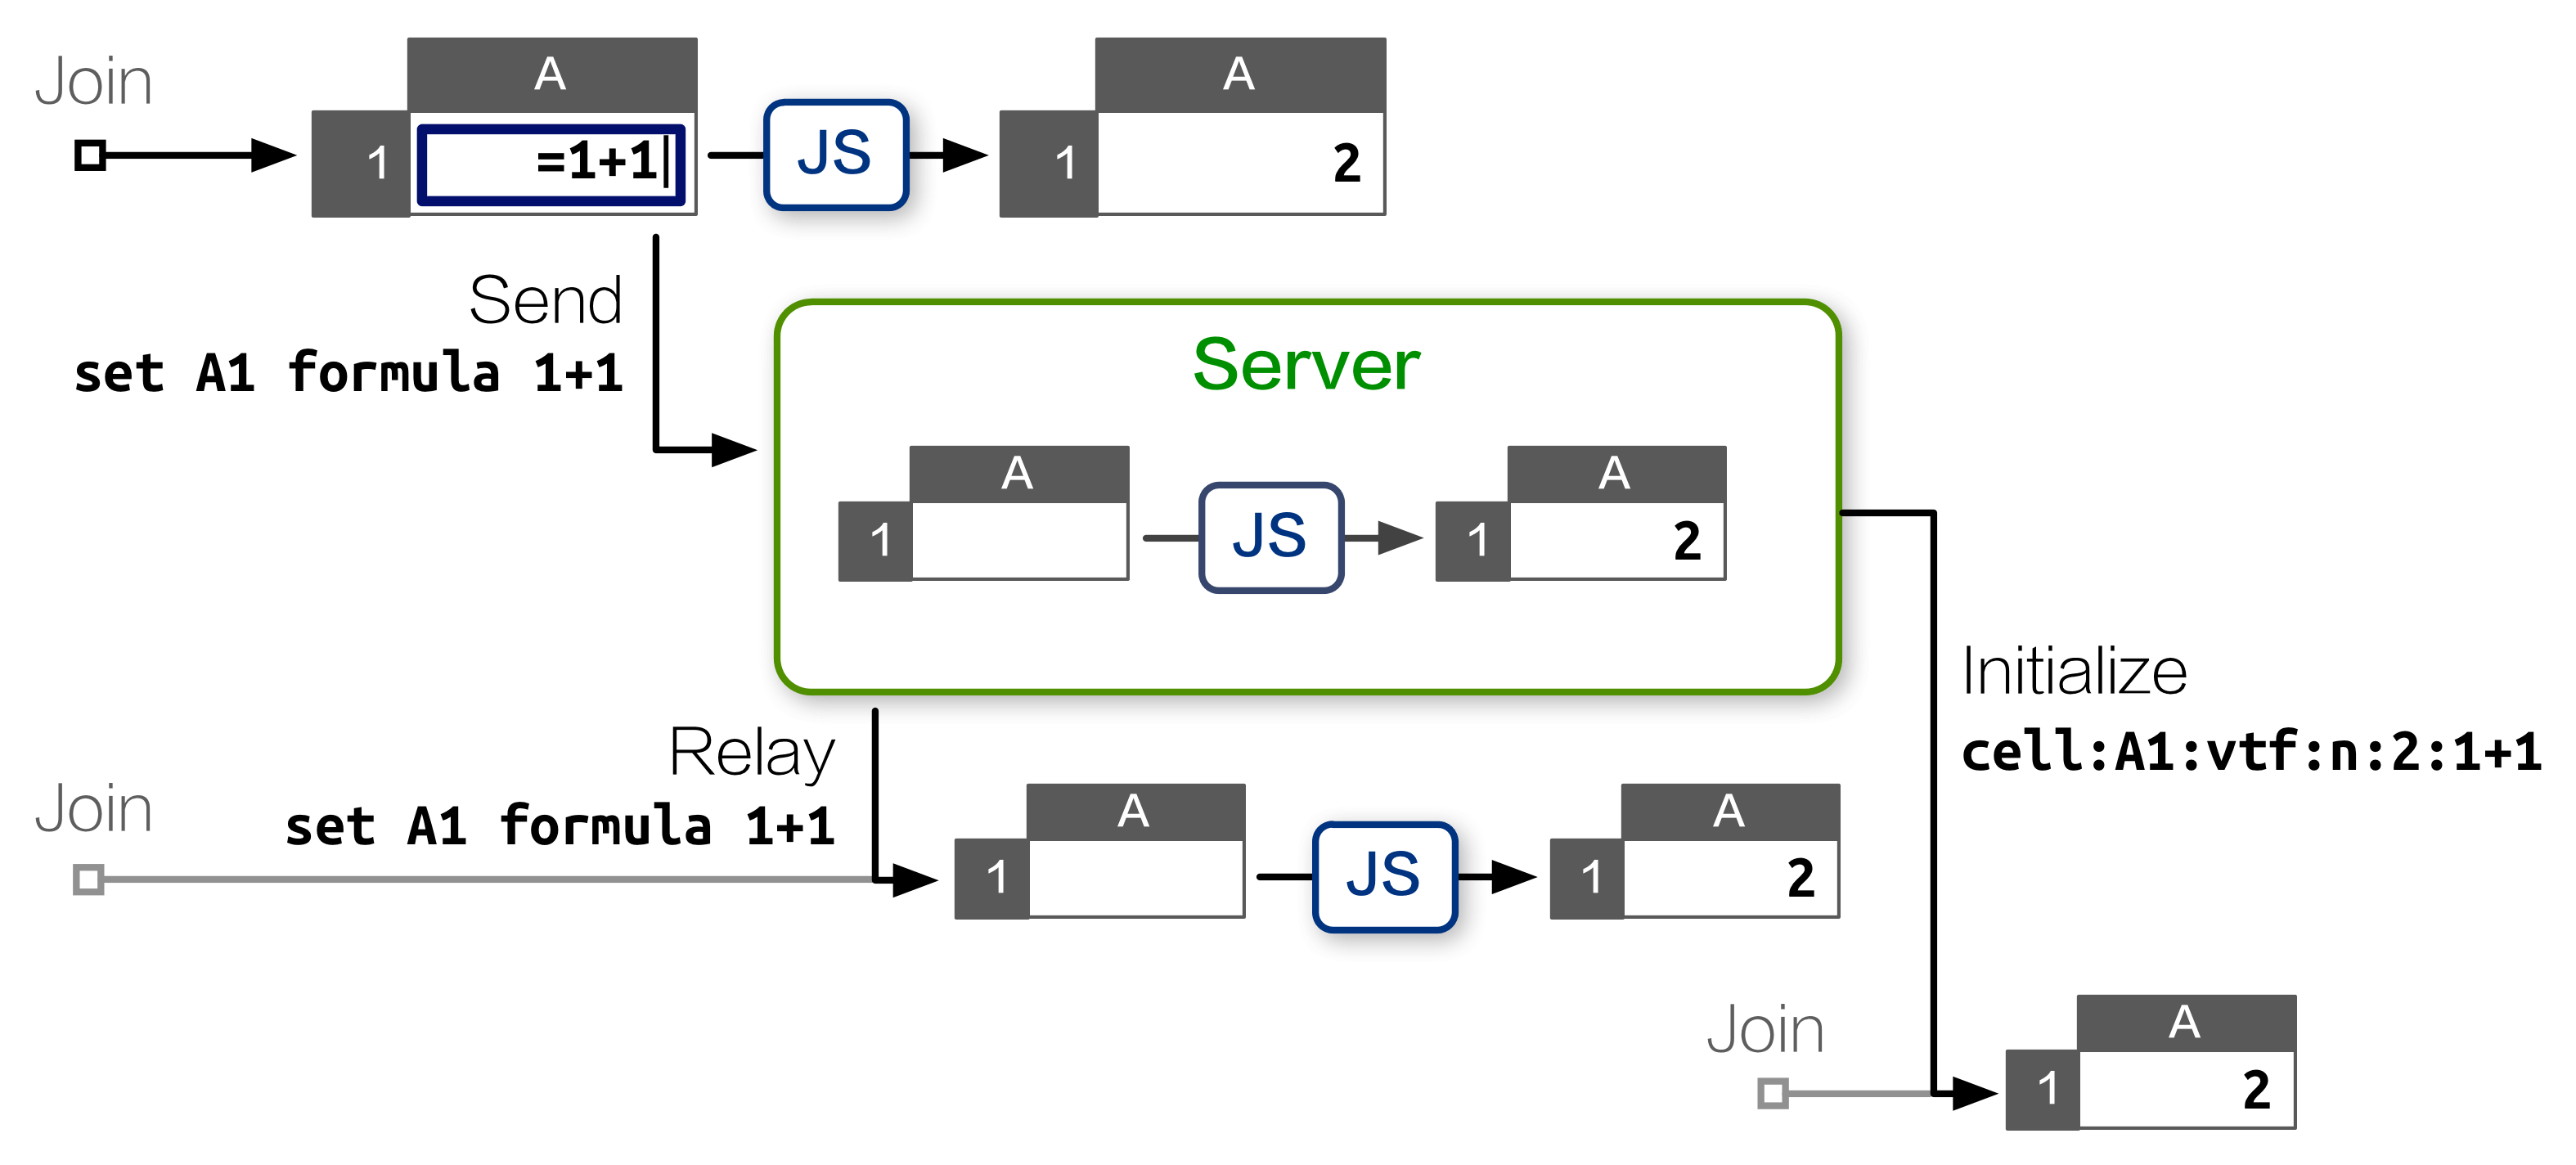
\includegraphics[width=0.6\textwidth]{resources/chapter-2-ethercalc.png}
        \caption{Ilustrasi Cara Kerja Kolaborasi pada EtherCalc}
        \label{IlustrasiEtherCalc}
    \end{figure}

    \subsubsection{Google Sheet}
    Google Sheet merupakan salah satu perangkat lunak pada \textit{office suite} miliki Google. Google Sheet dapat berjalan di atas tiga \textit{platform} yang berbeda yakni: sebagai \textit{web application}, Chrome apps, dan \textit{mobile apps}. Sheet memiliki kemampuan berkolaborasi secara \textit{real-time} dan menyediakan fitur-fitur \textit{spreadsheet} yang ada pada umumnya. Sheet memiliki fitur \textit{revision history} sehingga setiap orang dapat melihat perubahan yang terjadi, \textit{add-ons} yang dapat menambahkan fitur kepada Sheet melalui program yang dibuat oleh komunitas serta fitur \textit{chat} dengan kolaborator. Google Sheet dikembangkan menggunakan bahasa \textit{javascript} yang memberikan kemampuan penyimpanan dan kolaborasi secara \textit{real-time} \citep{GoogleSheet}.

    \subsubsection{OnlyOffice}
    Merupakan perangkat lunak sebagai \textit{service} yang dikembangkan oleh Ascensio System SIA. OnlyOffice merupakan \textit{office suite} yang berjalan di atas \textit{web application} yang dipadukan dengan sistem \textit{customer relationship management}. OnlyOffice tidak hanya terdiri dari \textit{online office editor} namun juga terdapat fitur managemen dokumen, manajemen proyek, \textit{mail service}, serta manajemen pelanggan seperti kontak, \textit{invoice}, \textit{opportonities}, dan \textit{task}. OnlyOffice ditujukan kepada bisnis yang membutuhkan perangkat lunak yang dapat mengorganisir kebutuhan bisnis di dalam satu aplikasi yang saling terintegrasi \citep{OnlyOffice}. 


\section{Penggunaan \textit{Spreadsheet}}
\textit{Spreadsheet} dapat digunakan untuk melakukan kalkulasi terhadap suatu rumus atau formula yang sulit jika dikalkulasikan dengan cara manual. Di samping itu, \textit{spreadsheet} dapat juga digunakan untuk melakukan ramalan terhadap suatu perubahan variabel masukan. Pada perkembangannya, \textit{spreadsheet} memiliki fitur-fitur tambahan seperti visualisasi data dan ekstraksi data penting dari kumpulan data yang ada.

Penelitian tentang penggunaan \textit{spreadsheet} pada bisnis pernah dilakukan sebelumnya pada tahun 2014. Subjek yang diteliti adalah akuntan manajemen \citep{Bradbard2014}. Pada penelitian tersebut, didapatkan gambaran umum mengenai penggunaan \textit{spreadsheet} secara umum. Menurut hasil penelitian tersebut beberapa fitur yang sering digunakan oleh pengguna \textit{spreadsheet} secara terurut dari yang paling sering digunakan adalah sebagai berikut,

\begin{enumerate}
    \item Menghitung fungsi matematika dasar (tambah, kurang, kali, bagi, dan lainnya)
    \item Mengelola \textit{worksheet} dan \textit{workbook} (menambahkan, menghapus, merubah nama, dan lainnya)
    \item Melakukan perubahan format dasar (menebalkan, memberi garis bawah, format angkat, dan lainnya)
    \item Melakukan pengurutan data, penghitungan subtotal, serta meringkas data
    \item Menggunakan fitur \textit{cell addressing} baik absolut maupun relatif
    \item Penggunaan fungsi kondisi (IF, COUNTIF), fungsi logika (AND, OR), fungsi pencarian (VLOOKUP, HLOOKUP), menautkan \textit{workbook} lain, serta fungsi pembulatan (ROUND, CEILING, FLOOR)
\end{enumerate}

Penggunaan \textit{spreadsheet} sangat bergantung kepada domain bisnis atau organisasi yang menggunakan. Pada bisnis yang berorientasi komersial, \textit{spreadsheet} dapat digunakan sebagai alat bantu perhitungan laba, pengeluaran, investasi, dan pajak. Pada organisasi-organisasi non komersial, \textit{spreadsheet} dapat digunakan sebagai salah satu bentuk basis data yang menangani penyimpanan, pengelolaan, dan pengumpulan data yang mudah dan cepat.

\section{Kesalahan dalam Penggunaan \textit{Spreadsheet}}
\subsection{Kualitas Data}
Kualitas Data (\textit{Data Quality}) adalah tingkat kemampuan data untuk memenuhi kebutuhan penggunaannya (\textit{usage requirement}) sehingga data dapat digunakan dengan baik \citep{Khatri2010}. Dimensi yang ada pada kualitas data dapat dibagi menjadi:

    \begin{enumerate}
        \item Akurasi, merujuk kepada tingkat kebenaran dari data.
        \item Aktualitas, menunjukan bahwa data yang dicatat merupakan data terbaru.
        \item Kelengkapan, menunjukkan bahwa nilai-nilai yang diperlukan tercatat (tidak hilang).
        \item Kredibilitas, menunjukkan kepercayaan terhadap sumber serta isinya.
    \end{enumerate}

Tingkatan nilai untuk dimensi tersebut dapat berbeda pada setiap kasus yang ada. Contohnya, akurasi 85\% untuk data nama dan alamat dokter merupakan nilai yang cukup baik bagi perusahaan asuransi yang menargetkan doktor sebagai konsumen potensial, namun tidak cukup baik untuk perusahaan obat yang ingin melakukan \textit{recall} terhadap obat yang terdistribusi. Kualitas data yang buruk dapat menyebabkan akibat yang fatal dalam bisnis baik secara operasional maupun strategis. 

\subsection{Tingkat Kesalahan dalam Penggunaan \textit{Spreadsheet}}
Penelitian telah dilakukan oleh Panko \citep{Panko1998} untuk mengetahui banyaknya kesalahan yang terjadi pada pengembangan \textit{spreadsheet} terutama pada sektor bisnis. Dari penelitian ini, didapatkan bahwa 20\% hingga 40\% \textit{spreadsheet} mengandung kesalahan. Pada kasus tertentu, bahkan ditemukan 90\% \textit{spreadsheet} yang diteliti memiliki kesalahan \citep{Journal1996}. 

Penelitian yang dilakukan oleh Panko juga menemukan 88\% dari 113 \textit{spreadsheet} yang diaudit melalui 7 lebih studi yang diteliti. Beberapa hasil yang telah di rangkum oleh penelitian tersebut mengunakan \textit{spreadsheet} yang digunakan di dunia nyata dapat dilihat pada Tabel \ref{StudiKesalahan}.
  \begin{small}
  \begin{longtable}{ | L{3cm} | R{2cm} | R{2cm} | R{2cm} | L{3cm} | }
    \caption{Studi terhadap Kesalahan pada \textit{Spreadsheet}}
    \label{StudiKesalahan}\\ \hline
    \centering\bfseries{Pembuat} & \centering\bfseries{Jumlah yang Diaudit} & \centering\bfseries{Rata-rata Sel} & \centering\bfseries{Persentase Error} & \centering\bfseries{Keterangan Kesalahan} \tabularnewline \hline
    \endfirsthead
    \hline
    \centering\bfseries{Pembuat} & \centering\bfseries{Jumlah yang Diaudit} & \centering\bfseries{Rata-rata Sel} & \centering\bfseries{Persentase Error} & \centering\bfseries{Keterangan Kesalahan} \tabularnewline \hline
    \endhead
    Butler (1992) & 273 & - & 11\% & Kesalahan perhitungan pada pajak\\ \hline
    Dent (1994) & Tidak diketahui & - & 30\% & Menggunakan angka yang ditulis manuals yang mengakibatkan perhitungan berikutnya salah\\ \hline
    Hicks (1995) & 1 & 3856 & 100\% & Kesalahan interpretasi pada data \\ \hline
    Coopers \& Lybrand (1997) & 23 & 150+ & 91\% & Kesalahan perhitungan yang meleset hingga 5\% \\ \hline
    Lukasic (1998) & 2 & 2270 - 7027 & 100\% & Kesalahan akibat melebih-lebihkan perhitungan hingga 16\%\\ \hline
    Clermont, Hanin, \& Mittermeier (2002) & 3 & - & 100\% & Kesalahan akibat perhitungan sel kosong\\ \hline
    Lawrence and Lee (2004) & 30 & 2182 & 100\%  & Kesalahan perhitungan dan formula\\ \hline
    Powell, Lawson, and Baker (2007) & 25 & - & 64\%  & Kesalahan perhitungan dan formula \\ \hline
    Powell, Baker \& Lawson (2007) & 50 & - & 86\%  & Kesalahan perhitungan dan formula \\ \hline
  \end{longtable}
  \end{small}
Dari kumpulan data di atas, dapat dilihat bahwa di dalam pembentukan \textit{spreadsheet} pada bidang bisnis, tidak mungkin terlepas dari kesalahan. Dengan tingginya tingkat kesalahan ini, bisnis dapat mengalami kerugian secara material maupun moral yang cukup besar \citep{EUSPRIGHorrorStories}. Hal ini mengindikasikan bahwa tingginya tingkat kesalahan harus dapat diselesaikan agar tidak terjadi kerugian di dalam penggunaan \textit{spreadsheet} terutama dalam bisnis.

\subsection{Tipe Kesalahan dalam Penggunaan \textit{Spreadsheet}} \label{KesalahanPenggunaan}
Tingkat fleksibilitas \textit{spreadsheet} yang tinggi memberikan keleluasaan kepada penggunanya untuk melakukan banyak manipulasi dan pengelolaan data. Tingginya fleksibilitas ini dapat berakibat mudahnya \textit{human error} terjadi pada saat penggunaan \textit{spreadsheet} yang menyebabkan terjadinya kesalahan-kesalahan pada data. Tipe-tipe kesalahan pada \textit{spreadsheet} dapat dibagi menjadi dua jenis tipe kesalahan yakni kesalahan kuantitatif, dan kesalahan kualitatif \citep{Panko1998}. 

    \subsubsection{Kesalahan Kualitatif}
    Kesalahan kualitatif merupakan kesalahan yang berhubungan dengan kualitas \textit{spreadsheet} tersebut lebih menitikberatkan pada kebiasaan dan prosedur yang salah di dalam pembuatan \textit{spreadsheet}. Beberapa kesalahan yang dapat diklasifikasikan sebagai kesalahan kualitatif adalah \citep{Powell2009}:

    \begin{enumerate}
        \item Melakukan \textit{hard-code} pada suatu angka di dalam formula
        \item Menggunakan formula yang panjang dalam perhitungan
        \item Susunan data yang tidak direncanakan dengan baik
        \item Tidak adanya dokumentasi mengenai \textit{spreadsheet} yang dibuat
    \end{enumerate}

    Kesalahan ini tidak langsung mengakibatkan nilai hasil keluaran yang salah namun menurunkan kualitas dari \textit{spreadsheet} tersebut \citep{Rajalingham2001}. Di samping itu, kesalahan kualitatif dapat menyebabkan kesalahan kuantitatif terutama pada saat penggunaan fungsi analisis \textit{what-if} pada \textit{spreadsheet} \citep{Panko1998}.

    \subsubsection{Kesalahan Kuantitatif}
    Kesalahan ini mengakibatkan \textit{spreadsheet} mengeluarkan hasil dan nilai yang salah di dalam operasi perhitungannya. Kesalahan jenis ini dapat dibagi menjadi empat jenis kesalahan \citep{Howe2006}, yakni:

    % \begin{enumerate}
    %     \item Kesalahan mekanikal (\textit{mechanical error}) yang biasanya terjadi akibat kesalahan pengetikan angka atau rujukan sel yang salah pada suatu formula
    %     \item Kesalahan logika (\textit{logical error}) yang terjadi pada pembuatan formula yang salah atau penggunaan fungsi yang tidak tepat
    %     \item Kesalahan akibat kelalaian pada interpretasi situasi atau spesifikasi yang diberikan sehingga \textit{spreadsheet} yang dihasilkan tidak sesuai dengan domain permasalahan yang ada atau \textit{ommision error} \citep{Powell2009}
    % \end{enumerate}

    \begin{enumerate}
        \item Kesalahan \textit{clerical} dan non-material merupakan kesalahan yang tidak berpengaruh pada hasil dan perhitungan, namun tetap merupakan kesalahan. Contohnya adalah kesalahan ejaan.
        \item \textit{Rule violations} merupakan kesalahan yang melanggar aturan yang telah ditetapkan. Contohnya nilai seseorang tidak boleh melebihi angka 100.
        \item Kesalahan \textit{data-entry} merupakan kesalahan yang terjadi saat memasukan data. Contohnya data yang seharusnya angka, namun dimasukkan berupa teks.
        \item Kesalahan \textit{formula}  merupakan kesalahan yang terjadi akibat penggunaan \textit{formula}. Kesalahan yang terjadi bisa berupa referensi tidak sesuai, penggunaan konstanta yang salah, atau kesalahan logika.
    \end{enumerate}

    Pada penelitian yang dilakukan oleh Howe, diketahui bahwa faktor yang berpengaruh terhadap ditemukannya kesalahan \textit{formula} adalah umur, indeks prestasi, serta pengalaman pemrograman. Sedangkan kesalahan lain, tidak dipengaruhi oleh faktor-faktor eksternal yang diuji. \citep{Howe2006} Hal ini juga terlihat pada penelitian yang dilakuakn oleh Bishop, dimana profesional lebih baik dalam mendeteksi kesalahan \textit{formula} hingga lebih baik 16\% dibandingkan orang kebanyakan. \citep{bishop2008empirical} Sehingga, dapat terlihat bahwa dengan pelatihan yang baik, kesalahan formula dapat berkurang, namun kesalahan lain tidak berkurang cukup signifikan.

% \subsection{Penanganan Kesalahan pada \textit{Spreadsheet}} \label{PenangananKesalahan}
% Untuk mengatasi kesalahan yang dijelaskan pada subbab sebelumnya, menurut penelitian yang dilakukan oleh Panko \citep{Panko1998}, dijabarkan beberapa metode untuk menangani dan mengurangi kesalahan yang sering terjadi. Beberapa metode yang dapat digunakan yakni:

%     \begin{enumerate}
%         \item Membangun \textit{preliminary design} sebelum pembuatan \textit{spreadsheet} agar terdapat perencanaan yang baik di dalam pembangunan data di dalam \textit{spreadsheet}
%         \item Melakukan proteksi terhadap sel yang tidak boleh diubah.
%         \item Melakukan pengecekan terhadap semua rumus dan formula yang dimasukan bahkan hingga rumus yang cukup sederhana dengan cara melakukan pengecekan manual.
%         \item Membuat dokumentasi untuk \textit{spreadsheet} yang dibuat.
%         \item Tidak menekan pembuat \textit{spreadsheet} terhadap kesalahan yang dibuat dengan memberikan hukuman. Kesalahan yang terjadi pada \textit{spreadsheet} umumnya masih berada pada batas normal \textit{human error} sehingga memberikan hukuman akan membuat rasa takut dalam melaporkan kesalahan.
%         \item Melakukan inspeksi terhadap formula, rumus, dan kode yang dibuat baik oleh individual maupun secara berkelompok.
%     \end{enumerate}

\section{Data pada \textit{Spreadsheet}} \label{JenisSpreadsheet}

\subsection{Tipe Struktur Data pada \textit{Spreadsheet}}
Pada penelitian yang dilakukan oleh Chen dan Cafarella, \textit{spreadsheet} dapat dibagi menjadi 2 jenis yakni; \textit{data frame} dan \textit{non-data frame}. \textit{Data frame} merupakan tipe \textit{spreadsheet} yang terdiri dari 2 komponen utama: area nilai dan area atribut atau metadata (biasanya berada di atas dan atau di kiri area nilai). \textit{Non-data frame} adalah tipe \textit{spreadsheet} selain tipe \textit{data frame} yang telah didefinisikan sebelumnya. Tipe \textit{non-data frame} dapat dibagi menjadi beberapa jenis yakni:

    \begin{enumerate}
        \item Relasi merupakan tipe \textit{spreadsheet} yang dapat langsung diubah ke model relasional.
        \item Formulir merupakan \textit{spreadsheet} yang tidak ditujukan sebagai penyimpanan dan didesain untuk diisi oleh manusia.
        \item Diagram yang digunakan sebagai visualisasi data, biasanya berisi banyak data tanpa skema informasi yang detil.
        \item Daftar atau \textit{List} merupakan catatan sejumlah nama atau hal (tentang kata-kata, nama orang, barang, dan sebagainya) yang disusun berderet dari atas ke bawah \citep{pusat1991kamus}.
        \item Jadwal merupakan \textit{spreadsheet} digunakan sebagai pembuatan dan pengelolaan jadwal.
        \item Silabus merupakan kerangka unsur kursus pendidikan, disajikan dalam aturan yang logis, atau dalam tingkat kesulitan yang makin meningkat \citep{pusat1991kamus}.
        \item \textit{Scorecard} yakni suatu alat manajemen yang biasanya berguna untuk membantu manajer melacak aktivitas yang dilakukan oleh stafnya.
    \end{enumerate}

Penelitian ini menggunakan sampel 200 \textit{spreadsheet} yang dilabeli oleh ahli dan didapatkan bahwa 50.5\% \textit{spreadsheet} merupakan tipe \textit{data frame}, dimana 32.5\% memiliki label atribut dibagian atas atau bawah. Sedangkan 49.5\% \textit{spreadsheet} bertipe \textit{non-data frame} terdiri dari 22.0\% relasi, 10.5\% formulir, 3.5\% diagram, 3\% berupa \textit{list}, dan 10.5\% lainnya \citep{Chen2013}.

\subsection{Pengolahan Data pada \textit{Spreadsheet}}
    \textit{Extract-Transform-Load} (ETL) adalah proses yang digunakan sebagai metode integrasi data dari beberapa sumber dan aplikasi. ETL biasanya digunakan pada saat melakukan proses \textit{data warehouse} dimana data dari sumber eksternal diambil, lalu ditransformasikan ke bentuk yang sesuai dengan kebutuhan (di dalam prosesnya bisa terkadung pengecekan kualitas), dan memasukannya ke dalam basisdata yang telah ditentukan \citep{Bansal2014}. Terdapat tiga fase pada proses ETL yakni:

    \begin{enumerate}
        \item \textit{Extract}, fase pertama ini adalah proses yang melakukan ekstraksi data dari sumber yang dipilih. Data biasanya tersedia dalam format \textit{flat file} seperti csv, xls, dan txt atau melalui klien RESTful.
        \item \textit{Transform}, pada fase ini data dibersihkan agar sesuai dengan skema tujuan. Beberapa cara untuk mentransformasikan data adalah dengan menormalisasi data, menghapus duplikasi, melakukan pengecekan terhadap batasan-batasan, melakukan \textit{filtering}, melakukan pengurutan dan pengelompokan, atau fungsi-fungsi lain yang didefinisikan.
        \item \textit{Load}, pada fase ini data yang telah ditransformasikan dimasukan ke dalam \textit{data mart} atau \textit{data warehouse} yang ditentukan.
    \end{enumerate}

    \subsubsection{Metode ETL pada \textit{Spreadsheet}} \label{metodepencarian}
    Pada penelitian yang dilakukan oleh Chen, pengolahan data pada sebuah \textit{spreadsheet} bertipe \textit{data frame} dapat dibagi menjadi tiga proses yakni: \textit{frame finder}, \textit{hierarchy extractor}, dan \textit{tuple builder}. Proses \textit{frame finder} dilakukan dengan cara mengidentifikasi \textit{data frame} serta mencari lokasi dari atribut dan nilai. Pada proses \textit{hierarchy extractor}, atribut yang ada pada \textit{data frame} yang ditemukan dicari hirarkinya setelah itu proses \textit{tuple builder} membentuk \textit{tuple} relasional untuk setiap nilai yang ada. Proses ini tidak membedakan \textit{spreadsheet} tipe \textit{data frame} atau bukan, sehingga diasumsikan jika \textit{tuple} yang dihasilkan memiliki kualitas yang baik, dapat dikatakan bahwa \textit{spreadsheet} masukan bertipe \textit{data frame} dan sebaliknya \citep{Chen2013}.

        \paragraph{\textit{Frame Finder}}
        Tujuan dari proses \textit{frame finder} \citep{Chen2013} adalah mengidentifikasi wilayah nilai dan wilayah atribut yang dapat berupa \textit{left attribute} maupun \textit{top attribute}. Untuk mensimplifikasi permasalahan, Chen menganggap bahwa \textit{data frame} tidak akan berada sejajar secara horisontal, namun hanya secara vertikal. Sehingga proses ini dapat disimplifikasi menjadi labeling terhadap baris per baris. Label yang akan diberikan adalah \textit{title}, \textit{header}, \textit{data}, dan \textit{footnote}.

        Pelabelan dapat dilakukan dengan algoritma \textit{conditional random field} (CRF) karena terdapat keterkaitan antara satu baris terhadap baris yang lain dalam penggunaan baris. Contohnya, jika baris telah teridentifikasi sebagai \textit{header}, maka besar kemungkinan bahwa baris selanjutnya adalah \textit{data} atau \textit{header}. CRF memiliki kemampuan untuk melakukan \textit{machine learning} yang memperhitungkan label pada elemen sebelumnya.

        \paragraph{\textit{Hierarcy Extractor}}
        Proses \textit{hierarcy extractor} \citep{Chen2013} bertujuan untuk mendapatkan hirarki dari atribut-atribut yang ada. Masukan dari proses ini adalah \textit{data frame} dengan \textit{top attribute} dan \textit{left attribute} dan keluarannya berupa hirarki untuk masing-masing atribut atas dan kiri tersebut. Proses ini dapat dilakukan melalui dua algoritma: \textit{classification} dan \textit{enforced-tree classification}.

        \textit{Classification} dilakukan dengan cara berbeda untuk \textit{left attribute} dan \textit{top attribute}. Pada \textit{left attribute}, klasifikasi dapat dilakukan dengan dua cara: pengecekan terhadap \textit{formatting} pada sebuah sel dan kedekatan sel secara geometris. Semakin mirip \textit{formatting} sebuah sel, maka semakin mungkin bahwa kedua sel bukan merupakan pasangan \textit{parent} dan \textit{child} dan semakin dekat sel secara geometris, kemungkinan kedua sel meruapakan  pasangan \textit{parent} dan \textit{child} semakin besar. Sedangkan pada \textit{top attribute} dapat dilakukan pengecekan posisi antar baris atribut bagian atas.

        Kelemahan pada metode klasifikasi sebelumnya adalah terdapat kemungkinan tidak dapat dibentuk pohon dari hasil klasifikasi. \textit{Enforced-tree classification} mencoba untuk menyelesaikan permasalahan ini dengan dua langkah tambahan yakni: memastikan bahwa suatu atribut hanya dapat memiliki satu \textit{parent} dimana yang terpilih menjadi \textit{parent} adalah atribut dengan probabilitas tertinggi, dan memastikan bahwa tidak ada \textit{cycle} yang terbentuk dengan cara menghapus keterhubungan dengan nilai probabilitas terkecil. Klasifikasi ini tetap menggunakan metode klasifikasi fitur yang dilakukan pada algoritma \textit{classification}.

        \paragraph{\textit{Tuple Builder}}
        Proses ini dilakukan dengan cara mengiterasi setiap \textit{value (v)} dan mencari atribut akar pada atribut bagian kiri dan atas dari \textit{v}. Setelah dibentuk \textit{relational tuple} untuk nilai \textit{v} dengan atribut bagian kiri dan atas tersebut. Tingkat akurasi dari proses ini sangat bergantung dari dua proses sebelumnya.

% \section{\textit{Data Governance}}
% Penggunaan \textit{spreadsheet} pada bisnis tidak terlepas dari adanya penyimpanan dan pengelolaan informasi. 

\section{Studi dan Penelitian Terkait}
    \subsection{\textit{Senbazuru: A Prototype Spreadsheet Database Management System}}
    Senbazuru \citep{Chen2013-2} merupakan prototipe yang dikembangkan dengan tujuan untuk mempermudah pencarian, pengaksesan, pengubahan, dan melakukan \textit{query} terhadap \textit{spreadsheet}. Pengembangan ini ingin menyelesaikan permasalahan dimana data \textit{spreadsheet} sangat tersebar diberbagai tempat sehingga untuk mendapatkan informasi yang diinginkan atau membandingkan antar informasi di dalam beberapa \textit{spreadsheet} sangatlah sulit. 

    Di dalam pengembangan prototipe ini, kesulitan teknikal yang harus dihadapi adalah proses ekstraksi dan perbaikan data. Di dalam melakukan ekstraksi data, harus dilakukan beberapa proses berikut: mendeteksi mana atribut dan nilai, mengidentifikasi hirarki atribut, membentuk \textit{relational tuple}, dan membentuk \textit{tuple} tersebut menjadi tabel relasional. Dari hasil dari ekstrasi ini, masih sangat mungkin memiliki kesalahan sehingga proses perbaikan diperlukan di dalam pembentukan tabel relasional ini. Proses perbaikan pada protitipe ini dilakukan manual dengan bantuan pengguna.

    \subsubsection{Arsitektur Sistem}

    \begin{figure}[!htb]
        \centering
        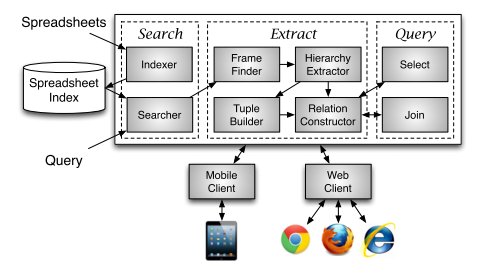
\includegraphics[width=0.7\textwidth]{resources/chapter-2-senbazuru-architecture.png}
        \caption{Arsitektur Sistem Senbazuru \citep{Chen2013-2}}
        \label{ArsiSisSenbazuru}
    \end{figure}

    \textit{Spreadsheet Database Management System} (SSDBMS) yang dikembangkan pada prototipe ini memiliki tiga proses utama yakni: \textit{search}, \textit{extract}, dan \textit{query}. Proses pencarian dilakukan terhadap repositori \textit{spreadsheet} yang ada di internet, lalu data \textit{spreadsheet} tersebut diekstraksi dan dijadikan tabel relasional, dan setelah itu pengguna dapat melakukan \textit{query} terhadap tabel yang telah dibentuk. Gambaran arsitektur Senbazuru dapat dilihat pada Gambar \ref{ArsiSisSenbazuru}. Arsitektur ini terbagi menjadi tiga modul utama yakni Search, Extract, dan Query.

        \paragraph{\textit{Search}}
        Komponen pencarian ini memudahkan pengguna untuk menemukan dataset yang tepat menggunakan bantuan internet. Saat prototipe ini dikembangkan, Senbazuru telah mengindeks 1800 \textit{spreadsheet} yang didapatkan dari U.S. Census Bureau. Pengindeksan menggunakan bantuan \textit{library} Python yakni xlrd untuk mengekstraksi teks dari sel lalu menggunakan Apache Lucene untuk melakukan indeks pada teks. Pencarian menggunakan metode \textit{term frequency–inverse document frequency} (TF-IDF) untuk mendapatkan relevansi dokumen.
        
        \paragraph{\textit{Extract}}
        Proses ekstraksi data pada \textit{spreadsheet} dilakukan melalui empat tahapan yakni:

        \begin{enumerate}
            \item \textit{Frame Finder}\\
            Tahap ini dilakukan untuk mencari \textit{frame} pada \textit{spreadsheet} bertipe \textit{data frame}. Dengan menggunakan algoritma \textit{conditional random field} (CRF) untuk memberikan label pada setiap baris yang tidak kosong pada \textit{spreadsheet}. Tahap ini akan menghasilkan \textit{data frame} yang selanjutnya akan digunakan pada tahap selanjutnya, baris lain yang dianggap bukan \textit{data frame} akan diabaikan.

            \item \textit{Hierarchy Extractor}\\            
            Tahap selanjutnya adalah ekstraksi hirarki pada wilayah atribut dari \textit{data frame} yang ditemukan. Pada setiap atribut, akan dicari atribut mana yang dideskripsikan oleh atribut lainnya dan seterusnya hingga terbentuk hirarki dari atribut-atribut yang ada. Kesalahan pada pembentukan hirarki sangat mungkin terjadi sehingga pengguna akan diberikan kemampuan untuk memperbaiki hirarki yang salah pada bagian \textit{repair interface}. Setelah perbaikan dilakukan oleh pengguna, Senbazuru akan menjalankan kembali CRF untuk melakukan pembelajaran terhadap label baru yang diberikan.

            \item \textit{Tuple Builder}\\            
            Bagian ini melakukan pembentukan \textit{tuple} antara wilayah nilai dan wilayah atribut yang sesuai.

            \item \textit{Relation Constructor}\\
            Tahap ini melakukan transalasi dari \textit{tuple} yang terbentuk menjadi tabel relasional dengan cara membentuk kluster terhadap atribut yang satu jenis. Contohnya, terdapat atribut \textit{Male}, \textit{total}, dan \textit{Female}, ketiga atribut tersebut memiliki jenis yang sama sehingga harus digabungkan menjadi satu kolom yakni \textit{gender}. Pada Senbazuru, teknik pengklusteran ini menggunakan bantuan koleksi skema dari Freebase dan YAGO.
        \end{enumerate}

        \paragraph{\textit{Query}}
        Setelah proses sebelumnya selesai, maka pengguna dapat memasukan perintah relasional terhadap data \textit{spreadsheet} yang telah diubah menjadi tabel relasional. Pada prototipe yang dikembangkan, perintah yang diimplementasikan adalah \textit{join} dan \textit{select}.

    \subsubsection{Hasil Penelitian}
    Senbazuru merupakan prototipe untuk manajemen basis data berbasis \textit{spreadsheet} yang dapat melakukan pencarian data pada internet melalui kata kunci yang diberikan. Prototipe ini berhasil melakukan ekstraksi data secara otomatis walaupun tidak terlepas dari kesalahan. Kesalahan yang terjadi masih harus seringkali dilakukan perbaikan secara manual. Namun dengan penggunaan algoritma CRF, protitipe dapat mengurangi kesalahan yang terjadi. Prototipe ini juga ditujukan sebagai demo kepada peserta konferensi VLDB dan diharapkan dapat menarik perhatian komunitas basis data.

\subsection{\textit{Spreadsheet As a Relational Database Engine}}
Penelitian \citep{Tyszkiewicz2010} pernah dilakukan terhadap pembuatan \textit{spreadsheet} menjadi mesin basis data relasional. Penelitian ini dilatarbelakangi dengan tingginya penggunaan \textit{spreadsheet} pada banyak bidang dan kurangnya kualitas data yang ada di dalamnya yang dapat menyebabkan kesalahan-kesalahan terjadi pada perhitungan dan prediksi. Solusi yang dipaparkan pada penelitian ini adalah dengan menggabungkan \textit{spreadsheet} dan \textit{database engine} dengan menggunakan formula sebagai ganti dari \textit{SQL query}.

    \subsubsection{Cara Kerja Sistem}

    Pada implementasinya, sebuah \textit{workbook} akan memiliki satu \textit{worksheet} untuk setiap tabel data dan satu \textit{worksheet} untuk setiap \textit{view} pada basis data. Dengan menggunakan \textit{external compiler} yang menerima masukan berupa SQL yang akan mengubahnya ke dalam bentuk \textit{spreadsheet}. Program tersebut akan mengubah SQL menjadi beberapa formula yang diterima oleh \textit{spreadsheet} tersebut.

    Terdapat dua bagian utama pada \textit{spreadsheet} hasil implementasi yakni: tabel data dan bagian \textit{view}. Bagian tabel data adalah tempat pengguna untuk memasukkan, mengubah, serta menghapus data. Secara teori, bagian tabel data tidak memiliki formula, namun di dalam implementasinya mengikuti implementasi SQL dimana perlu dilakukan validasi data dan verifikasi terhadap \textit{primary key}, \textit{foreign key}, dan batasan lain yang ada diperintah \textit{create table}.

    Bagian \textit{view worksheet} tidak dapat diubah oleh pengguna dan berisikan formula-formula yang independen terhadap data yang dimasukkan oleh pengguna. Di samping itu, bagian \textit{view} berisikan kolom-kolom yang berguna sebagai \textit{intermediate result} yang selanjutnya akan digunakan oleh formula lain. Pada awalnya sel-sel akan berisikan "" (\textit{string} kosong) yang merepresentasikan sel yang belum digunakan.

    \subsubsection{Hasil Penelitian}

    Formula pada excel dilakukan menggunakan \textit{linear scan} dan hal ini dapat mengurangi kinerja. Beberapa cara untuk meningkatkan kinerja adalah mengeksploitasi \textit{lazy evaluation} dari \textit{if statement}, mengkomputasi hanya beberapa sel tetangga yang berkaitan, serta menggunakan file atau \textit{workbook} lain untuk membagi \textit{query} dan membangkitkannya ketika dibutuhkan.

    Pada tes kinerja yang dilakukan pada penelitian ini dapat disimpulkan bahwa untuk operasi dasar dan \textit{query} sederhana penggunaan \textit{spreadsheet} dapat digunakan dengan baik dengan waktu yang cukup cepat. Tingkat efektifitas penggunaan pada arsitektur ini cukup rendah, namun hasil tes tersebut menunjukan bahwa arsitektur ini memiliki potensial yang dapat dikembangkan.
    \chapter{Analisis Masalah Pengumpulan Data Pada \textit{Spreadsheet}}

Pada bab ini diuraikan analisis persoalan pengumpulan data pada \textit{spreadsheet} yang telah diuraikan pada Bab I. Hasil dari bab ini digunakan untuk merancang kakas yang akan diimplementasikan seperti yang dijelaskan pada Bab IV.

\section{Permasalahan Pengumpulan Data Pada \textit{Spreadsheet}} \label{AspekAplikasi}
Pada Subbab \ref{RumusanMasalah} telah dijelaskan bahwa terdapat tiga permasalahan yang muncul dalam pengumpulan data menggunakan media \textit{spreadsheet} yakni:
\begin{enumerate}
	\item Kolaborasi \\
	Dalam pembuatan suatu \textit{spreadsheet}, kadang dibutuhkan banyak pihak untuk dapat melengkapi seluruh data yang dibutuhkan. Hal ini membuat pengembangan dan pengumpulan data membutuhkan kontribusi banyak orang \citep{Panko1998}. Untuk itu dibutuhkan fitur kolaborasi pada aplikasi \textit{spreadsheet} agar banyak pihak dapat melakukan pengumpulan data dan pengeditan secara bersamaan.
	\item Validasi \\
	Data yang dikumpulkan pada suatu \textit{spreadsheet}, sangat rentan akan kesalahan. Bahkan pada \textit{spreadsheet} yang dibuat dengan sangat hati-hati, masih dapat ditemui sekitar 1 persen atau lebih kesalahan pada formula yang dibuat \citep{Panko1998}. Sehingga dibutuhkan mekanisme tambahan pada saat pengumpulan data untuk melakukan validasi terhadap masukan.
	\item Penyimpanan Data \\
	Setelah data dikumpulkan, permasalahan selanjutnya yang muncul adalah penyimpanan data tersebut. Data biasanya akan tetap tersimpan dalam bentuk berkas \textit{spreadsheet}, namun bentuk ini sulit untuk digunakan oleh aplikasi lain. Bentuk yang biasanya digunakan oleh aplikasi lain untuk dapat mengambil dan menyimpan data adalah bentuk relasional. Sehingga dibutuhkan mekanisme penyimpanan data ke dalam bentuk relasional agar data dapat dengan mudah digunakan pada aplikasi lain.
\end{enumerate}

Ketiga permasalahan tersebut yang dijadikan dasar pengembangan kakas pada Tugas Akhir ini dan akan dibahas pada subbab-subbab berikutnya. 

% Pada Subbab \ref{KesalahanPenggunaan} dijelaskan bahwa terdapat dua jenis kesalahan yang dapat terjadi pada penggunaan \textit{spreadsheet} yakni kesalahan kualitatif dan kesalahan kuantitatif. Kesalahan kualitatif merupakan kesalahan penggunaan \textit{spreadsheet} yang berhubungan dengan kualitas dan prosedur penggunaan. Contoh kesalahan kualitatif yang sering terjadi adalah penggunaan \textit{spreadsheet} sebagai basis data. Kesalahan kuantitatif merupakan kesalahan yang menyebabkan keluaran menjadi salah. Contoh kesalahan kuantitatif yang sering terjadi adalah kesalahan masukan yang tidak divalidasi.

% Pencegahan untuk kesalahan-kesalahan ini dapat dilihat pada Subbab \ref{PenangananKesalahan}. Salah satu caranya adalah pembuatan \textit{preliminary design} terhadap \textit{spreadsheet} yang dibuat. Hal ini dapat dilakukan dengan cara pengembangan aplikasi pengumpulan data berbentuk \textit{spreadsheet} yang menangani kolaborasi, validasi, dan penyimpanan. Dengan aplikasi ini diharapkan dapat menangani kesalahan kualitatif seperti yang dijelaskan pada contoh sebelumnya yakni penggunaan \textit{spreadsheet} sebagai basis data dengan cara menghubungkan \textit{spreadsheet} ke basis data yang sesungguhnya secara langsung. Serta menangani kesalahan kuantitatif dengan cara melakukan validasi masukan.

% Aplikasi \textit{spreadsheet} yang baik harus dapat diakses dan digunakan secara kolaboratif yang dapat dilakukan dengan membuat aplikasi \textit{spreadsheet} tersebut berbasis \textit{web}. Aspek-aspek aplikasi \textit{web} yang perlu diperhatikan dalam membangun aplikasi \textit{spreadsheet} adalah:
% \begin{enumerate}
% 	\item \textit{Response time}\\
% 	Membangun aplikasi berbasis \textit{web} menggunakan HTTP sebagai protokol komunikasi dan tentunya didalam komunikasi tersebut membutuhkan waktu untuk mengirimkan \textit{request} dari klien. Jika waktu yang dibutuhkan untuk melakukan respon lambat, akan sulit terjadi kolaborasi dan memperbesar kemungkinan terjadinya \textit{race condition} pada masukan pengguna. Sehingga diperlukan waktu respon yang cepat untuk dapat menangani banyak \textit{request} dalam satu waktu dan dalam waktu yang singkat.

% 	\item Akses yang konkuren\\
% 	Aplikasi berbasis \textit{web} yang akan dibuat harus dapat diakses secara konkuren yakni diakses bersama-sama oleh banyak klien dalam satu waktu. Pengaksesan secara konkuren dapat berdampak pada terpanggilnya banyak \textit{query} dalam satu waktu. Oleh karena itu aplikasi yang dibuat harus dapat menjalankan secara konkuren setiap \textit{request} yang masuk.

% 	\item Akses basis data\\
% 	Akses terhadap basis data dibutuhkan sebagai media penyimpanan yang persisten dan konsisten. Oleh karena itu, akses terhadap basis data diperlukan untuk kemudahan penyimpanan dan pengambilan data serta mengatasi permasahalan ketidaksamaan \textit{versioning} diantara suatu \textit{file spreadsheet}.

% \end{enumerate}

% Keempat aspek pada aplikasi berbasis \textit{web} tersebut akan menjadi aspek utama yang dikembangkan didalam pembuatan aplikasi \textit{spreadsheet} berbasis aplikasi \textit{web}.

% Berdasarkan pada Subbab \ref{KesalahanPenggunaan}, terdapat dua jenis tipe kesalahan \citep{Panko1998} yang bisa terjadi pada penggunaan \textit{spreadsheet} yakni:
% \begin{enumerate}
% 	\item Kesalahan Kualitatif

% 	Kesalahan kualitatif merupakan kesalahan yang berhubungan dengan kualitas yang dipengaruhi oleh prosedur pembuatan dan rancangan pada \textit{spreadsheet} tersebut. Contoh kesalahan kualitatif yang sering terjadi adalah penggunan \textit{spreadsheet} sebagai media penyimpanan atau basis data. Hal ini tidak sesuai dengan kegunaan utama dari \textit{spreadsheet} sebagai media kalkulasi dan perhitungan statistik.

% 	\item Kesalahan Kuantitatif

% 	Kesalahan kuantitatif merupakan kesalahan yang menyebabkan hasil perhitungan menjadi salah atau tidak valid. Contoh kesalahan jenis ini yang sering terjadi adalah kesalahan mekanikal dimana pengguna salah memasukan data yang tidak sesuai dengan konstrain yang ada. Hal ini dapat diatasi dengan adanya validasi sebelum data diterima. 
% \end{enumerate}

% Dari kedua tipe tersebut, pada Tugas Akhir ini akan lebih ditekankan kepada kesalahan kuantitatif yang bertipe kesalahan mekanikal dengan memanfaatkan teknik validasi pada masukan. 

% Dengan menggunakan aplikasi ini, terdapat perubahan alur penggunaan \textit{spreadsheet}. Gambar dibawah ini merupakan alur penggunaan aplikasi \textit{spreadsheet} biasa pada Gambar \ref{GambarWorkflowBiasa} dan aplikasi \textit{spreadsheet} yang dibangun pada Tugas Akhir ini pada Gambar \ref{GambarWorkflow}. 

% 	\begin{figure}[htb]
% 	    \centering
% 	    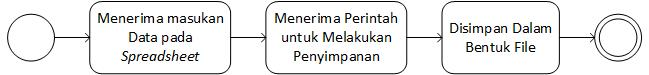
\includegraphics[width=0.7\textwidth]{resources/chapter-3-workflow-biasa.jpg}
% 	    \caption{Alur Kerja Aplikasi \textit{Spreadsheet} Biasa}
% 		\label{GambarWorkflowBiasa}
% 	\end{figure}

% 	\begin{figure}[htb]
% 	    \centering
% 	    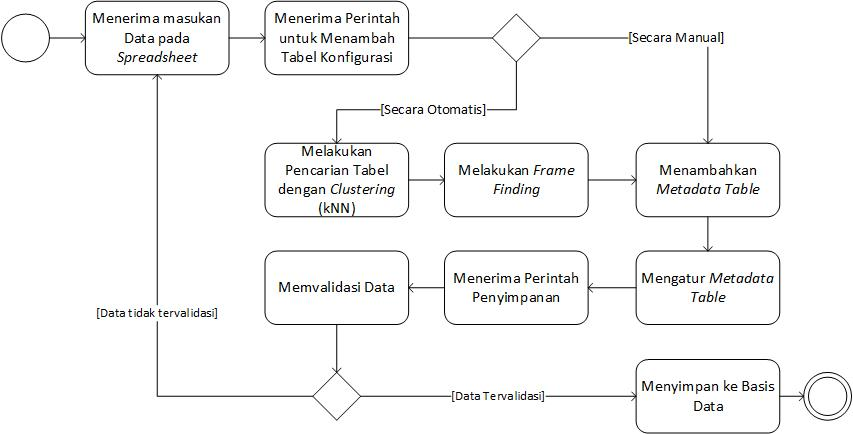
\includegraphics[width=1\textwidth]{resources/chapter-3-workflow.jpg}
% 	    \caption{Alur Kerja Aplikasi \textit{Spreadsheet} yang Akan Dibuat}
% 		\label{GambarWorkflow}
% 	\end{figure}

% Dapat dilihat bahwa terdapat proses tambahan yang dilakukan pada aplikasi yang akan dibuat. Proses tersebut terdiri dari pencarian bagian label dan data serta proses validasi. Hasil dari identifikasi label dan data akan dijadikan \textit{tuple} relasional yang disimpan dalam bentuk basis data.

\section{Analisis Rancangan Kakas pada Aplikasi \textit{Spreadsheet}}
Dari permasalahan yang telah didefinisikan pada subbab \ref{AspekAplikasi}, dapat ditentukan beberapa hal yang harus dianalisis dalam merancang kakas pada aplikasi \textit{spreadsheet} ini, diantaranya adalah:
\begin{enumerate}
	\item Penentuan aplikasi \textit{spreadsheet} yang akan dikembangkan dan ditambahkan fiturnya. Aplikasi harus memiliki fitur kolaborasi sehingga banyak pengguna dapat mengakses suatu \textit{spreadsheet} secara bersamaan.
	\item Penanganan konflik yang terjadi pada saat kolaborasi.
	\item Jenis \textit{spreadsheet} yang menjadi fokus utama untuk dapat ditangani oleh kakas.
	\item Pemilihan metode interaksi kakas pada aplikasi \textit{spreadsheet} dimana pengguna dapat membentuk struktur tempat pengguna lain memasukkan masukan. Contohnya dalam bentuk tabel atau formulir. Pengguna juga melengkapi domain dan batasan data yang dimasukkan.
	\item Setelah pengguna selesai merancang struktur masukan, diperlukan penentuan bagian label dan data yang berkaitan dengan label tersebut. Bagian label dan data akan dijadikan menjadi bentuk relasional yang dapat disimpan dalam basis data.
	\item Setelah label dan data ditentukan, tabel harus direpresentasikan dalam bentuk relasional sehingga dapat dimasukkan ke dalam basis data.
	\item Setelah data dikumpulkan, data perlu divalidasi dan dicek kesesuaiannya sesuai dengan batasan yang diberikan sehingga memenuhi domain yang ditentukan pada basis data.
	\item Setelah proses validasi terpenuhi, diperlukan cara penyimpanan data sesuai dengan relasi \textit{tuple} yang telah ditentukan.
	\item Interaksi antar \textit{spreadsheet} yang ingin memasukkan data pada suatu tabel yang sama perlu ditangani dan ditentukan aturannya.
\end{enumerate}
Pada subbab-subbab selanjutnya, akan dibahas analisis untuk kelima poin di atas yang selanjutnya akan dijadikan dasar rancangan kakas yang akan dibuat pada aplikasi \textit{spreadsheet}.

\section{Analisis Perbandingan Aplikasi \textit{Spreadsheet} yang Dikembangkan}
Dari studi yang telah dilaksanakan pada subbab \ref{TeknologiSpreadsheet}, aplikasi \textit{spreadsheet} dapat dibagi berdasarkan konektivitasnya yakni \textit{offline spreadsheet} dan \textit{online spreadsheet} dan dapat juga dibagi lagi berdasarkan keterbukaan dari \textit{source code} yakni \textit{open source} dan \textit{closed source}. Pada Tabel \ref{AnalisisAplikasiDasar} dijabarkan parameter yang mendasari pemilihan aplikasi yang akan dikembangkan.

\begin{small}
\begin{longtable}{ | p{3cm} | p{4cm} | p{4cm} | }
    \caption{Perbandingan Aplikasi \textit{Spreadsheet}}
    \label{AnalisisAplikasiDasar}\\ \hline
    \centering\bfseries{Parameter} & \centering\bfseries{Offline Application} & \centering\bfseries{Web/Online Application} \tabularnewline \hline
    \endfirsthead
    \hline
    \centering\bfseries{Parameter} & \centering\bfseries{Offline Application} & \centering\bfseries{Web/Online Application} \tabularnewline \hline
    \endhead
    Aksesibilitas & Dibutuhkan instalasi aplikasi / plugin yang bersangkutan. & Dapat menggunakan web browser yang tersedia. \\ \hline
    Kolaborasi & Tidak tersedia secara online dan kolaboratif secara \textit{default}. & Secara \textit{default}, dapat diakses konkuren dan kolaboratif. \\ \hline
    Fitur & Sudah banyak jenis formula yang didukung. & Tidak semua formula yang ada didukung. \\ \hline
\end{longtable}
\end{small}

Dari perbandingan di atas, diambil solusi dengan menggunakan aplikasi \textit{spreadsheet} berbasis web yang dapat diakses secara konkuren dan memiliki \textit{portability} yang lebih baik. Di samping itu, untuk dapat mengembangkan fitur aplikasi dengan lebih baik, akan dipilih aplikasi yang berbentuk \textit{open source}. Alasan lain dipilihnya \textit{open source} adalah aplikasi berbasis \textit{open source} dapat dipasang pada \textit{platform} yang diinginkan oleh pengguna. Pengguna atau perusahaan yang menggunakan aplikasi dapat membangun infrastrukturnya sendiri sehingga dapat mengatur privasi dan performa aplikasi sesuai dengan keinginan pengguna. Sehingga dipilih aplikasi yang memiliki tipe \textit{online spreadsheet} dan \textit{open source} yaitu EtherCalc. Fitur kolaborasi yang dibutuhkan akan ditangani oleh aplikasi EtherCalc ini dan bukan merupakan bagian dari fitur yang akan dikembangkan.

\section{Analisis Penanganan Konflik saat Kolaborasi}

\begin{figure}[!htb]
    \centering
    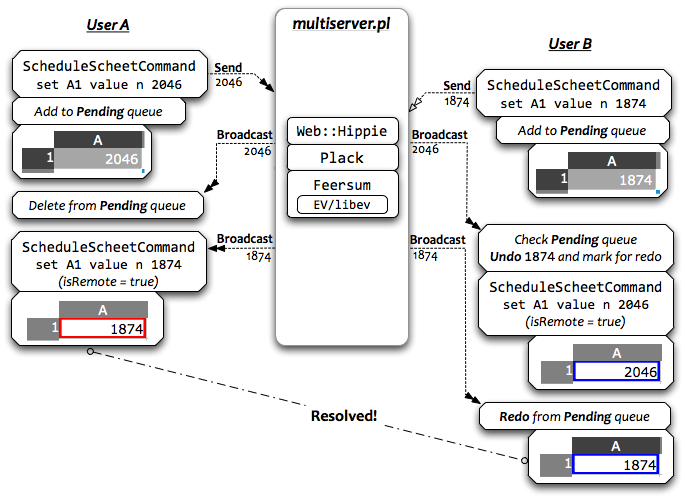
\includegraphics[width=1\textwidth]{resources/chapter-3-conflict-res.png}
    \caption{Mekanisme Penanganan Konflik \citep{EtherCalc}}
	\label{MekanismeKonflik}
\end{figure}

Penanganan konflik pada saat lebih dari satu pengguna memasukkan data pada suatu \textit{spreadsheet} yang sama telah ditangani oleh EtherCalc menggunakan mekanisme \textit{conflict resolution} yang berasal dari SocialCalc. Mekanisme penanganan konflik menggunakan fitur \textit{undo}/\textit{redo} yang telah ada. Gambaran mekanisme tersebut dapat dilihat pada Gambar \ref{MekanismeKonflik}. Berdasarkan gambaran tersebut dan \textit{website} resmi dari EtherCalc, langkah-langkah penanganan konflik yang terjadi adalah sebagai berikut:

\begin{enumerate}
	\item Ketika klien mengirimkan suatu perintah. Perintah tersebut dimasukkan ke \textit{pending queue}.
	\item Ketika klien menerima \textit{broadcast} perintah, akan dilakukan pengecekan \textit{pending queue}.
	\item Jika \textit{pending queue} kosong, maka perintah akan langsung dijalankan.
	\item Jika perintah baru sama dengan \textit{pending queue}, perintah akan dijalankan dan dihapus dari \textit{pending queue}.
	\item Jika tidak, maka dilakukan pengecekan apakah terjadi konflik.
	\item Jika terjadi konflik, maka akan dilakukan perintah \textit{Undo} dan ditandai untuk dilakukan \textit{Redo} pada saat konflik terselesaikan.
	\item Setelah semua konflik terselesaikan, jalankan perintah seperti biasa.
	\item Jika masih terdapat perintah yang ditandai untuk dilakukan \textit{Redo}, maka perintah tersebut dijalankan kembali.
\end{enumerate}

\section{Analisis Jenis \textit{Spreadsheet} yang Ditangani}
Pada Subbab \ref{JenisSpreadsheet} telah dijelaskan jenis-jenis \textit{spreadsheet} yang biasanya dibuat. Persentase jenis \textit{spreadsheet} terbesar yang dibuat berjenis \textit{data frame} dengan persentase 50.5\%. \textit{Data frame} merupakan tipe \textit{spreadsheet} yang terdiri dari 2 komponen utama: area nilai dan area atribut atau metadata (biasanya berada di atas dan atau di kiri area nilai). Karena tingginya angka penggunaan menggunakan tipe ini, kakas akan melakukan penanganan pada \textit{spreadsheet} bertipe \textit{data frame}.

Persentase kedua ditempati oleh jenis \textit{spreadsheet} bertipe relasi yang memiliki persentase 22.0\%. Tipe relasi ini merupakan tipe \textit{spreadsheet} yang dapat langsung diubah ke model relasional. Biasanya berupa satu \textit{header} dan kumpulan baris data. Dengan tingginya persentase tipe ini serta miripnya tipe relasi dan \textit{data frame}, tipe ini juga dipilih untuk dapat ditangani oleh kakas.

Tipe lainnya yang teridentifikasi adalah tipe formulir, diagram, dan jadwal. Ketiga jenis ini memiliki penanganan yang berbeda-beda dan tidak memiliki sifat yang sama dengan tipe \textit{data frame} dan relasi. Sehingga, tipe ini tidak dijadikan fokus dalam pengembangan kakas untuk dapat ditangani. Dengan menangani hanya tipe \textit{data frame} dan relasi diharapkan telah dapat menangani 72.5\% kasus penggunaan \textit{spreadsheet} yang biasanya ditemui.

\section{Analisis Metode Interaksi Pengguna}
Di dalam pembangunan perangkat lunak \textit{spreadsheet} untuk mengurangi kesalahan, dapat diidentifikasikan dua metode interaksi yang dapat diimplementasi. Model interaksi yang pertama adalah menggunakan formulir sebagai basis masukan data dan metode yang kedua adalah menggunakan aplikasi \textit{spreadsheet} secara langsung sebagai media input data.
	\subsection{Berbasis Formulir}
	Metode interaksi ini menggunakan \textit{spreadsheet} sebagai tempat perancangan formulir. Pembuat formulir akan menentukan area label dan input secara manual serta diidentifikasikan berdasarkan warna atau properti lain yang unik pada sel tersebut. Formulir akan dibangkitkan oleh aplikasi agar menjadi bentuk HTML dan terhubung ke basis data. Pengisian data oleh pengguna dilakukan melalui formulir yang dibangkitkan dan dapat diakses melalui web. Beberapa cara dapat dilakukan untuk mengimplementasikan teknik ini antara lain, mengembangkan dari aplikasi \textit{spreadsheet} yang telah ada menggunakan \textit{plugin} atau membuat aplikasi baru yang dapat melakukan konversi otomatis menjadi formulir.

	\subsection{Berbasis \textit{Spreadsheet}}
	Metode interaksi berbasiskan \textit{spreadsheet} menggunakan antarmuka yang telah disediakan oleh aplikasi. Penggunaannya dilakukan dengan membuat format pengisian seperti membuat tabel pada \textit{spreadsheet} pada umumnya. Pada tabel harus terdapat label dan data sehingga metadata minimal yang dibutuhkan dapat dicapai. Fitur-fitur yang ada pada \textit{spreadsheet} juga tetap dapat digunakan saat pembuatan tabel yang diinginkan. Dari pembuatan tabel tersebut dilakukan identifikasi label dari data tersebut untuk selanjutnya diproses melalui penyaringan masukan dan dimasukan ke tabel yang sesuai yang ada di basis data. Untuk mengimplementasikan teknik ini harus mengubah kode pada program \textit{spreadsheet} atau mengekstensi fitur yang ada menggunakan \textit{plugin}. 

	\subsection{Perbandingan Metode Masukan}
	Kedua metode interaksi pengguna tersebut memiliki beberapa perbedaan dan efek terhadap penggunaannya baik bagi aplikasi maupun pengguna. Pada Tabel \ref{ModelInteraksi} dijabarkan perbandingan antara kedua metode interaksi pengguna tersebut.

	\begin{small}
	\begin{longtable}{ | p{3cm} | p{4cm} | p{4cm} | }
	    \caption{Perbandingan Metode Interaksi Pengguna}
	    \label{ModelInteraksi}\\ \hline
	    \centering\bfseries{Parameter} & \centering\bfseries{Berbasis Formulir} & \centering\bfseries{Berbasis \textit{Spreadsheet}} \tabularnewline \hline
	    \endfirsthead
	    \hline
	    \centering\bfseries{Parameter} & \centering\bfseries{Berbasis Formulir} & \centering\bfseries{Berbasis \textit{Spreadsheet}} \tabularnewline \hline
	    \endhead
	    Fungsionalitas & Berhasil memisahkan bagian operasional dan data. Pengguna hanya memodifikasi dan melakukan input pada bagian data. Bagian operasional hanya dapat dimodifikasi oleh pembuat formulir tersebut. & Jika tidak menggunakan proteksi terhadap sel yang dapat ditulis, tidak terjadi pemisahan antara data dan operasional sehingga beberapa kesalahan yang terjadi pada saat input masih dapat terjadi. \\ \hline
	    Teknologi & Dibutuhkan adanya algoritma tambahan untuk menangani formulir dan masukannya, serta melakukan konversi dan \textit{parsing} dari sel pada \textit{spreadsheet} ke dalam bentuk formulir. & Dibutuhkan algoritma dan logika \textit{parsing} yang lebih detil dan kompleks dalam menangani kasus-kasus table tertentu. \\ \hline
	    Antarmuka & Menggunakan antarmuka formulir yang kaku terurut dari atas ke bawah serta tidak dapat melihat hasil masukan secara langsung. & Struktur tabel atau masukan dapat disesuaikan dengan kebutuhan dan tidak perlu mempelajari hal lain jika sebelumnya telah menggunakan \textit{spreadsheet} sebagai media untuk memasukan data. \\ \hline
  	\end{longtable}
	\end{small}

  	Pada Tugas Akhir ini, akan dipilih metode masukan pengguna dengan berbasis \textit{spreadsheet} sehingga pengguna dapat dengan lebih mudah di dalam menggunakannya karena tidak memerlukan pembelajaran kembali di dalam menggunakan aplikasi. Di samping itu, data yang dimasukan lebih mudah untuk dilihat secara menyeluruh dibandingkan dengan berbasis formulir yang hanya dapat menerima satu masukan dalam suatu formulir.

\section{Analisis Penentuan Bagian Data dan Label}
Pada pembuatan \textit{spreadsheet} pada umumnya, didapatkan bahwa kebanyakan \textit{spreadsheet} pada umumnya berbentuk tabel yang terdiri dari dua unsur utama yakni data dan label atau disebut juga tipe \textit{data frame} \citep{Chen2013}. Bagian data merupakan bagian yang biasanya dinamis dan merupakan masukan pengguna. Bagian label merupakan bagian yang memberikan keterangan dan konteks mengenai data yang dimaksud. Pada Gambar \ref{DataFrameSederhana} dapat dilihat bahwa area dengan nomor 1 disebut sebagai label yang menjelaskan data dibawahnya yakni pada area nomor 2.

\begin{figure}[htb]
    \centering
    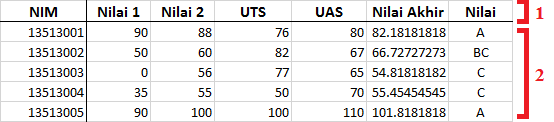
\includegraphics[width=0.7\textwidth]{resources/chapter-3-simple-dataframe2.png}
    \caption{Contoh \textit{Data Frame} Sederhana}
	\label{DataFrameSederhana}
\end{figure}

	\subsection{Secara Manual}
	Penentuan label dan data dilakukan oleh pengguna secara langsung saat pembuatan tabel. Pengguna sendiri yang menentukan area mana yang merupakan label dan data mana yang dijelaskan oleh label tersebut. Dengan metode manual ini, pengguna dapat menyesuaikan bentuk tabel sesuai keinginan mereka. Metode ini menyerahkan sepenuhnya tanggungjawab keterhubungan sel label dan sel data kepada pengguna. Metode yang digunakan adalah menerima masukan dari pengguna berupa suatu \textit{script} yang mendefinisikan letak tabel, \textit{header}, dan data pada \textit{spreadsheet}.

	\subsection{Secara Otomatis}
	Penentuan secara otomatis dimulai dari pencarian tabel pada \textit{spreadsheet}. Hal ini dilakukan karena tabel dapat lebih dari satu pada sebuah \textit{spreadsheet}. Penentuan tabel dilakukan menggunakan algoritma k-Nearest Neighbour (kNN) sehingga ditemukan kedekatan antar sel, lalu mengelompokkannya sehingga diketahui koordinat sel mana saja yang merupakan suatu kesatuan tabel. Setelah tabel ditemukan, pencarian label dan data dapat menggunakan algoritma seperti yang telah dijelaskan pada Subbab \ref{metodepencarian}. 

	Mekanisme yang akan diimplementasi pada kakas ini hanya bagian \textit{frame finder} yang bertujuan untuk mengidentifikasi wilayah nilai (data) dan wilayah atribut (label) yang dapat berupa \textit{left attribute} maupun \textit{top attribute}. Teknik \textit{frame finder} menggunakan algoritma pembelajaran mesin \textit{conditional random field} (CRF) yang dapat mendeteksi kemungkinan jenis data dengan mengetahui urutan kemunculan dan ketetanggaan antar data. Algoritma ini dilatih menggunakan data latih yang berasal dari \textit{Statistical Abstract of the United States} (SAUS) 2010 \citep{ChenGithub}. Dengan ditemukannya tabel-tabel pada \textit{spreadsheet} beserta label dan data yang ada pada tabel tersebut, seluruh \textit{metadata} tersebut ditampilkan dalam bentuk \textit{metadata table}.

	% Tahap selanjutnya adalah \textit{hierarchy extractor} bertujuan untuk mendapatkan hirarki dari atribut-atribut yang ada sehingga label yang tertulis dapat dicari keterhubungan dan konteksnya terhadap data yang ada. Tahap terakhir adalah \textit{tuple builder} yang mentrasformasikan data dan label tersebut dalam bentuk \textit{tuple} yang dapat diterima oleh basis data relasional.

	\subsection{Perbandingan Metode Penentuan}
	Untuk mengetahui perbandingan kedua metode, pada Tabel \ref{MetodePenentuan} dijelaskan kelebihan dan kekurangan dua metode yang telah disebutkan sebelumnya.
	\begin{small}
	\begin{longtable}{ | p{3cm} | p{4cm} | p{4cm} | }
	    \caption{Perbandingan Metode Penentuan Data dan Label}
	    \label{MetodePenentuan}\\ \hline
	    \centering\bfseries{Keterangan} & \centering\bfseries{Manual oleh Pengguna} & \centering\bfseries{Otomatis} \tabularnewline \hline
	    \endfirsthead
	    \hline
	    \centering\bfseries{Keterangan} & \centering\bfseries{Manual oleh Pengguna} & \centering\bfseries{Otomatis} \tabularnewline \hline
	    \endhead
	    Kelebihan & Tingkat akurasi lebih tinggi karena data dan label yang ditentukan sesuai dengan keinginan pengguna. & Kenyamanan dalam penggunaan karena pengguna tidak perlu melakukan interferensi tambahan. Di samping itu, kemungkinan data dan label yang diambil dapat diubah ke dalam bentuk \textit{tuple} relasional lebih tinggi. \\ \hline
	    Kekurangan & Interferensi pengguna yang banyak dan mungkinnya data dan label tidak dapat dijadikan bentuk \textit{tuple} relasional. & Algoritma ini hanya optimal jika digunakan pada tabel yang terurut vertikal. \\ \hline
  	\end{longtable}
	\end{small}
  	Dari perbandingan di atas, dapat dilihat terdapat kekurangan dan kelebihan di dalam menggunakan salah satu metode tersebut. Berdasarkan hal tersebut, yang akan dipilih sebagai metode penentuan data dan label adalah gabungan dari kedua metode tersebut. Kakas awalnya akan melakukan \textit{parsing} terhadap struktur yang telah dibuat oleh pengguna, kemudian pengguna dapat melihat hasil dari \textit{parsing} tersebut sehingga pengguna dapat memperbaiki jika terdapat hasil pelabelan yang salah. Dengan metode gabungan ini diharapkan dapat meningkatkan akurasi dan mengurangi kesalahan \textit{parsing} yang terjadi namun tetap memberikan kenyamanan terhadap pengguna serta menjaga agar hasil pelabelan tetap dapat diubah ke dalam bentuk \textit{tuple} relasional.

\section{Analisis Representasi Tabel pada \textit{Spreadsheet}}
Dalam pembuatan \textit{spreadsheet}, terdapat beberapa jenis tabel yang biasanya dibuat oleh pengguna dalam merepresentasikan data yang ingin disimpan. Pada jenis-jenis tabel tertentu, dibutuhkan transformasi bentuk tabel tersebut agar dapat dimasukkan ke dalam basis data bentuk relasional. Tipe-tipe tabel yang biasanya muncul di dalam pembuatan \textit{spreadsheet} beserta teknik transformasi yang akan digunakan adalah sebagai berikut:
\begin{enumerate}
	\item Tabel dengan \textit{header} berada di atas data
	\begin{figure}[htbp]
	    \centering
	    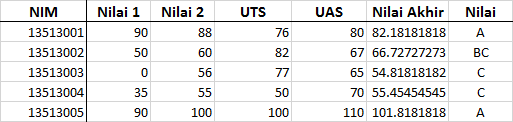
\includegraphics[width=0.8\textwidth]{resources/chapter-3-tabletype-1.png}
	    \caption{Tabel dengan \textit{Header} Berada Di atas Data}
		\label{TabelTipe1}
	\end{figure}\\
	Representasi tabel jenis ini dapat langsung dibuat ke dalam bentuk relasional tanpa harus mengubah struktur tabel. Contoh tabel jenis ini dapat dilihat pada Gambar \ref{TabelTipe1}. Bagian \textit{header} merupakan baris pertama pada tabel, dan baris kedua hingga seterusnya merupakan bagian data. Bentuk ini tidak membutuhkan transformasi agar dapat dimasukkan ke dalam basis data bentuk relasional.

	\item Tabel dengan \textit{header} berada di kiri dan atas data
	\begin{figure}[htbp]
	    \centering
	    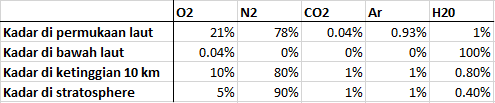
\includegraphics[width=0.8\textwidth]{resources/chapter-3-tabletype-2.png}
	    \caption{Tabel dengan \textit{Header} Berada di Kiri dan Atas Data}
		\label{TabelTipe2}
	\end{figure}\\
	Tabel dapat memiliki lebih dari satu \textit{header} di lokasi yang berbeda. Contoh tabel jenis ini dapat dilihat pada Gambar \ref{TabelTipe2}. Representasi tabel dimana \textit{header} bukan hanya di bagian atas saja, maka \textit{header} yang dianggap hanya yang di bagian atas. Bagian yang akan dianggap sebagai \textit{header} adalah kolom yang keseluruhannya berisi \textit{header} dan berada di atas data. Pada contoh di atas, \textit{header} adalah baris pertama. Sedangkan \textit{header} di kiri tabel yang satu baris dengan data akan dianggap data dengan nama \textit{header} yang dapat ditentukan oleh pengguna. Dengan demikian, representasi tabel tersebut akan menjadi mirip dengan tipe tabel sebelumnya. Representasi tabel setelah transformasi dapat dilihat pada Gambar \ref{TabelTipe2T}.\\
	\begin{figure}[htbp]
	    \centering
	    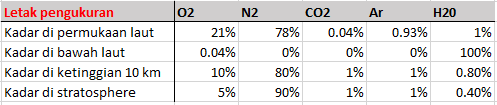
\includegraphics[width=0.8\textwidth]{resources/chapter-3-tabletype-2-transformed.png}
	    \caption{Transformasi Tabel dengan \textit{Header} Berada di Kiri dan Atas Data}
		\label{TabelTipe2T}
	\end{figure}

	\item Tabel dengan \textit{header} yang berhirarki
	\begin{figure}[htbp]
	    \centering
	    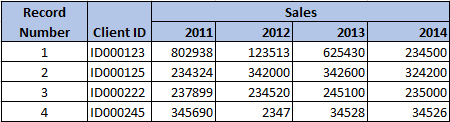
\includegraphics[width=0.7\textwidth]{resources/chapter-3-tabletype-3.png}
	    \caption{Tabel dengan \textit{Header} yang Berhirarki}
		\label{TabelTipe3}
	\end{figure}\\
	Tabel dapat memiliki \textit{header} yang berhubungan satu dengan yang lain dan membentuk hirarki seperti pada contoh Gambar \ref{TabelTipe3}. Tabel dengan \textit{header} yang memiliki hirarki akan tetap dianggap memiliki satu baris \textit{header}. Transformasi yang dilakukan adalah dengan menggabungkan kata-kata pada tiap \textit{header} dan dijadikan sebagai satu nama \textit{header} dan secara \textit{default} dipisahkan dengan tanda '\_' untuk masing-masing \textit{header}. Penggunaan tanda '\_' dan bukan spasi dilakukan agar pengguna dapat membedakan bagian yang merupakan hasil gabungan. Hasil transformasi tabel tersebut dapat dilihat pada Gambar \ref{TabelTipe3T}.\\
	\begin{figure}[htbp]
	    \centering
	    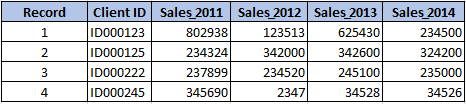
\includegraphics[width=0.75\textwidth]{resources/chapter-3-tabletype-3-transformed.png}
	    \caption{Transformasi Tabel dengan \textit{Header} yang Berhirarki}
		\label{TabelTipe3T}
	\end{figure}

	\item Tabel dengan data yang digabung
	\begin{figure}[htbp]
	    \centering
	    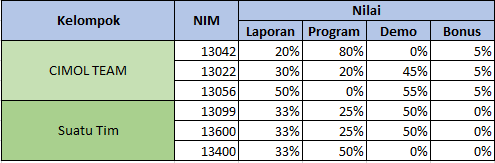
\includegraphics[width=0.8\textwidth]{resources/chapter-3-tabletype-4.png}
	    \caption{Tabel dengan Data yang Digabung}
		\label{TabelTipe4}
	\end{figure}\\
	Tabel dapat juga memiliki penggabungan sel pada bagian data seperti yang dapat dilihat pada contoh Gambar \ref{TabelTipe4}. Penggabungan sel ini biasanya digunakan sebagai penanda bahwa data pada setiap baris atau kolom yang digabung adalah sama. Sehingga, transformasi yang akan dilakukan adalah dengan memecah sel yang digabungkan tersebut dan mengisi setiap sel dengan konten yang sama dengan sel yang digabungkan. Hasil transformasi tabel dapat dilihat pada Gambar \ref{TabelTipe4T}.\\
	\begin{figure}[htbp]
	    \centering
	    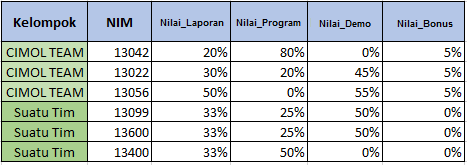
\includegraphics[width=0.75\textwidth]{resources/chapter-3-tabletype-4-transformed.png}
	    \caption{Transformasi Tabel dengan Data yang Digabung}
		\label{TabelTipe4T}
	\end{figure}
\end{enumerate}
Setelah ditransformasikan, tabel akan dapat dengan mudah dijadikan \textit{tuple} relasional sehingga dapat langsung dimasukkan ke dalam basis data relasional yang dipilih.

\section{Analisis Validasi Data}
Mekanisme validasi data bertujuan untuk menghindari kesalahan masukan. Berdasarkan pada penelitian \citep{Panko1998}, terdapat dua jenis tipe kesalahan yang bisa terjadi pada penggunaan \textit{spreadsheet} yakni kesalahan kualitatif dan kesalahan kuantitatif. Dari kedua tipe tersebut, Tugas Akhir ini lebih menekankan kepada kesalahan kuantitatif. Kesalahan kuantitatif diambil karena merupakan jenis kesalahan yang dapat ditangani oleh kakas, sedangkan jenis kesalahan kualitatif lebih berkaitan pada aturan dan konvensi pembuatan \textit{spreadsheet}.

Berdasarkan penelitian \citep{Howe2006}, diketahui bahwa pengurangan kesalahan \textit{formula} sangat dipengaruhi oleh faktor-faktor eksternal yang dapat diselesaikan jika berlatih dan terbiasa. Namun, jenis kesalahan lain tidak dipengaruhi oleh faktor-faktor ini, sehingga tingkat kesalahan yang terjadi cukuplah konsisten tidak tergantung pengalaman. Sehingga, jenis kesalahan yang akan ditangani oleh kakas ini akan lebih difokuskan pada kesalahan-kesalahan yang sulit dihilangkan bahkan jika pengguna telah berpengalaman.

Jenis kesalahan yang akan ditangani adalah kesalahan \textit{clerical} dan non-material, \textit{rule violations}, dan kesalahan \textit{data-entry}. Dari kesalahan-kesalahan tersebut, maka terdapat tiga hal utama yang divalidasi pada kakas ini, yakni:
\begin{enumerate}
	\item Validasi tipe data. Untuk pengembangan Tugas Akhir ini, hanya diimplementasi empat jenis validasi tipe data yakni \textit{integer}, \textit{double}, \textit{string}, dan \textit{boolean}. Contoh kasus validasi adalah ketika data masukan yang seharusnya berupa \textit{integer} tidak dapat menerima masukan berupa \textit{string}.
	\item Validasi domain masukan. Pada pengembangan Tugas Akhir ini, hanya diimplementasi validasi domain yang berupa aturan \textit{range}, lebih besar, lebih kecil, sama dengan, dan nilai diskrit. Aturan validasi juga hanya terbatas hanya satu aturan pada satu atribut pada \textit{metadata table}.
	\item Validasi relasi data. Data masukan dapat berupa nilai yang harus ada pada tabel lain, contohnya terdapat 2 tabel yakni nilai mahasiswa dan identitas mahasiswa. Tabel nilai mahasiswa memiliki kolom NIM yang nilainya harus ada pada tabel identitas mahasiswa. Pada \textit{spreadsheet} biasanya hal ini diatasi dengan menggunakan perintah VLOOKUP.
\end{enumerate}

Kesalahan \textit{clerical} dan non-material diharapkan dapat ditangani menggunakan validasi tipe data dan domain masukan. Kesalahan \textit{data-entry} dan \textit{rule violations} diharapkan dapat ditangani menggunkan validasi tipe data, validasi domain, dan validasi relasi data.

Kakas akan melakukan validasi terhadap ketiga hal tersebut dan menolak data masukan sehingga pengguna dapat memperbaiki data. Validasi akan dilakukan pada saat data akan dimasukkan ke dalam basis data. Letak validasi ini dapat dilihat pada alur pengumpulan data pada Subbab \ref{Aluralur}.

\section{Analisis Penyimpanan Data}
Terdapat tiga permasalahan pada penyimpanan data yang perlu dianalisis yakni; jenis penyimpanan data yang digunakan, alur pengguna melakukan penyimpanan data tersebut, dan perubahan pada data di basis data. Kedua masalah ini akan dijelaskan pada dua subbab berikut.

	\subsection{Jenis Penyimpanan Data} \label{JenisPenyimpanan}
	Terdapat 2 jenis data yang harus disimpan ke dalam basis data di dalam membangun kakas menggunakan aplikasi \textit{spreadsheet} ini, yakni:

	\begin{enumerate}
		\item Penyimpanan \textit{File Spreadsheet} \\
		\textit{File spreadsheet} yang dimaksud adalah data struktural seperti \textit{value} pada suatu sel, \textit{properties} suatu sel seperti warna, \textit{border}, dan \textit{alignment}, serta hal-hal lain yang berhubungan dengan bagaimana suatu \textit{file spreadsheet} ditampilkan pada aplikasi. Tipe penyimpanan yang dapat digunakan untuk menampung data ini adalah NoSQL karena tipe ini cocok untuk menangani data yang kurang terstruktur seperti \textit{file spreadsheet} yang struktur penempatan datanya berbeda tiap pengguna. Cara penyimpanan yang cocok untuk menangani struktur ini adalah \textit{document based} atau \textit{key-value}. Sehingga proses penyimpanan \textit{file spreadsheet} akan menggunakan mekanisme yang sudah disediakan oleh aplikasi EtherCalc dengan menggunakan redis.

		\item Penyimpanan Data dan Label \\
		Tipe penyimpanan yang cocok digunakan adalah basis data relasional (SQL) karena data yang dibuat dalam bentuk tabel pada umumnya dapat dikonversikan menjadi \textit{tuple} relasional. Data dan label yang telah ditentukan menggunakan \textit{metadata table} dijadikan bentuk yang dapat diterima basis data relasional. Label akan dijadikan nama kolom pada basis data, dan data akan dijadikan dalam bentuk baris-baris.

		% Data yang disimpan merupakan hasil dari pendeteksian label dan data yang akan diubah menjadi bentuk relasional yang dapat diterima oleh basis data relasional. Contoh pengubahan yang terjadi dapat dilihat pada Gambar \ref{RelationalTuple}.

		% \begin{figure}[htb]
		%     \centering
		%     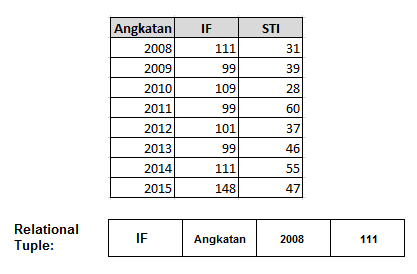
\includegraphics[width=0.6\textwidth]{resources/chapter-3-relational-tuple.png}
		%     \caption{Contoh \textit{Tuple} Relasional}
		% 	\label{RelationalTuple}
		% \end{figure}

		% Setelah data dan label dijadikan \textit{tuple} relasional, \textit{tuple} dimasukan ke dalam basis data dengan menggunakan operasi \textit{insert} ke dalam tabel pada basis data. Tipe penyimpanan yang cocok digunakan adalah basis data relasional (SQL) karena data yang dibuat dalam bentuk tabel pada umumnya dapat dikonversikan menjadi \textit{tuple} relasional.
	\end{enumerate}

	\subsection{Alur Penyimpanan Data}
	Dengan adanya dua jenis penyimpanan yang digunakan seperti telah dijelaskan pada Subbab \ref{JenisPenyimpanan} terdapat dua kemungkinan alur penyimpanan data, yakni:
	\begin{enumerate}
		\item Penyimpanan ke basis data dilakukan setiap mendapatkan masukan pengguna
		\item Penyimpanan ke basis data menunggu perintah dari pengguna
	\end{enumerate}

	Pada Tabel \ref{ModelAlurPenyimpanan} dijabarkan perbandingan antara kedua kemungkinan alur penyimpanan data tersebut.

	\begin{small}
	\begin{longtable}{ | p{3cm} | p{4cm} | p{4cm} | }
	    \caption{Perbandingan Alur Penyimpanan}
	    \label{ModelAlurPenyimpanan}\\ \hline
	    \centering\bfseries{Parameter} & \centering\bfseries{Dilakukan Setiap Mendapat Masukan} & \centering\bfseries{Menunggu Perintah Pengguna} \tabularnewline \hline
	    \endfirsthead
	    \hline
	    \centering\bfseries{Parameter} & \centering\bfseries{Dilakukan Setiap Mendapat Masukan} & \centering\bfseries{Menunggu Perintah Pengguna} \tabularnewline \hline
	    \endhead
	    Sinkronisasi & Data yang ada pada basis data yang menyimpan \textit{file spreadsheet} yakni redis dan data pada basis data relasional tersinkronisasi setiap saat. & Data diantara kedua basis data tidak selalu sinkron setiap saat. \\ \hline
	    Kinerja & Kinerja yang akan menurun diakibatkan kakas pendeteksian label dan data yang harus dilakukan setiap saat menerima masukan. & Kinerja yang lebih baik dibandingkan alur sebelumnya karena penyimpanan dilakukan \textit{on demand} \\ \hline
	    Akses penyimpanan & Sulit untuk mengembangkan aplikasi menggunakan \textit{user access control} karena sulit menentukan kapan dan oleh siapa data boleh dimasukkan ke dalam basis data. & Mengembangkan aplikasi dengan \textit{user access control} akan lebih mudah untuk menentukan siapa yang memiliki akses untuk melakukan penyimpanan.\\ \hline
  	\end{longtable}
	\end{small}

	Dari pertimbangan tersebut, alur yang dipilih adalah penyimpanan ke basis data yang menunggu perintah dari pengguna karena kelebihannya pada sisi performa dan \textit{user access control}. Di samping itu, tidak sinkronnya antara kedua basis data bukan merupakan masalah karena data yang ingin dikumpulkan merupakan data akhir dan data tiap perubahan yang dilakukan tidak begitu dipedulikan.

	\subsection{Perubahan pada Data di Basis Data}
	Kasus yang dapat terjadi pada basis data tempat penyimpanan data yang berasal dari \textit{spreadsheet} adalah diubahnya data tersebut secara manual oleh entitas lain. Pada kakas yang dibuat, kakas hanya bekerja sebagai media untuk mengumpulkan data sehingga perubahan yang terjadi pada basis data, tidak akan ditampilkan kembali menjadi bentuk \textit{spreadsheet} pada aplikasi. Di samping itu, perubahan data langsung pada basis data tanpa melalui media yang disediakan sangat tidak disarankan.

\section{Analisis Interaksi antar \textit{Spreadsheet}}
Interaksi yang akan dibahas terdiri dari dua jenis yakni interaksi data dan interaksi penyimpanan. Pada interaksi data akan dijelaskan bagaimana data pada dua atau lebih \textit{spreadsheet} dapat saling berinteraksi dalam bentuk fragmen. Sedangkan pada interaksi penyimpanan akan dijelaskan bagaimana aplikasi menyelesaikan permasalahan konflik penyimpanan yang terjadi akibat interaksi dua atau lebih \textit{spreadsheet}.

\subsection{Interaksi Data}
Data yang dikumpulkan pada dua atau lebih \textit{spreadsheet} dapat diklasifikasikan menjadi empat tipe berdasarkan fragmen data yang dikumpulkan yakni; tidak berhubungan, horizontal, vertikal, dan gabungan.

\begin{enumerate}
	\item Fragmen Tidak Berhubungan\\
	Dua atau lebih \textit{spreadsheet} dapat dikatakan tidak saling berpotongan fragmennya jika \textit{spreadsheet} tersebut tidak menyimpan data pada tabel yang sama pada basis data. Pada kasus tersebut, data pada kedua atau lebih \textit{spreadsheet} dapat dianggap tidak saling melengkapi dan dapat berdiri sendiri.
	
	\item Fragmen Horizontal\\
	Fragmen horizontal terjadi ketika dua atau lebih \textit{spreadsheet} menyimpan pada tabel basis data yang sama dimana data yang disimpan memiliki jumlah, nama, dan konteks kolom yang sama. Pada kasus tersebut, data pada dua atau lebih \textit{spreadsheet} akan digabungkan pada satu tabel yang sama secara horizontal. Contoh gambaran pengabungan data dapat dilihat pada Gambar \ref{HorizontalMerge}.

	\begin{figure}[!htb]
	    \centering
	    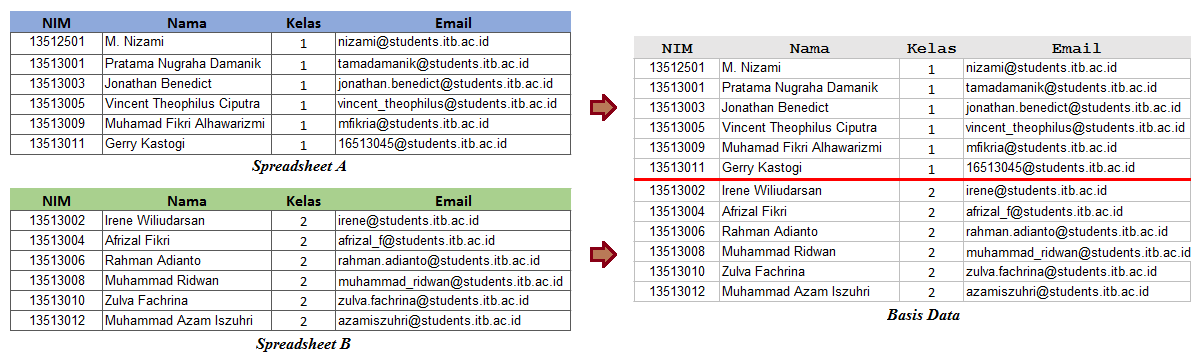
\includegraphics[width=1\textwidth]{resources/chapter-3-horizontal-merge.png}
	    \caption{Contoh Penggabungan Horizontal}
		\label{HorizontalMerge}
	\end{figure}

	Pada gambar, data pada \textit{spreadsheet} A dan \textit{spreadsheet} B digabungkan pada satu tabel pada basis data secara horizontal (diilustrasikan dengan garis merah). Pada kasus tersebut, NIM tidak didefinisikan sebagai nilai yang unik, sehingga jika terdapat NIM yang sama pada lebih dari satu \textit{spreadsheet} maka data akan tetap digabungkan secara horizontal pada data yang sudah ada bukan menulis kembali nilai pada NIM yang bersesuaian. Namun, jika nilai NIM didefinisikan sebagai unik, maka jika NIM terdapat di lebih dari satu \textit{spreadsheet} akan ditimpa dan ditulis kembali nilainya pada NIM yang sesuai.

	\item Fragmen Vertikal\\
	Fragmen vertikal terjadi ketika dua atau lebih \textit{spreadsheet} menyimpan pada tabel basis data yang sama dimana data yang disimpan memiliki satu kolom unik dengan nama dan konteks yang sama dan kolom lainnya dapat berbeda dari segi jumlah , nama, dan konteks di masing-masing \textit{spreadsheet}. Pada kasus ini, data pada dua atau lebih \textit{spreadsheet} akan digabungkan pada satu tabel yang sama secara vertikal. Contoh gambaran pengabungan data dapat dilihat pada Gambar \ref{VerticalMerge}.

	\begin{figure}[!htb]
	    \centering
	    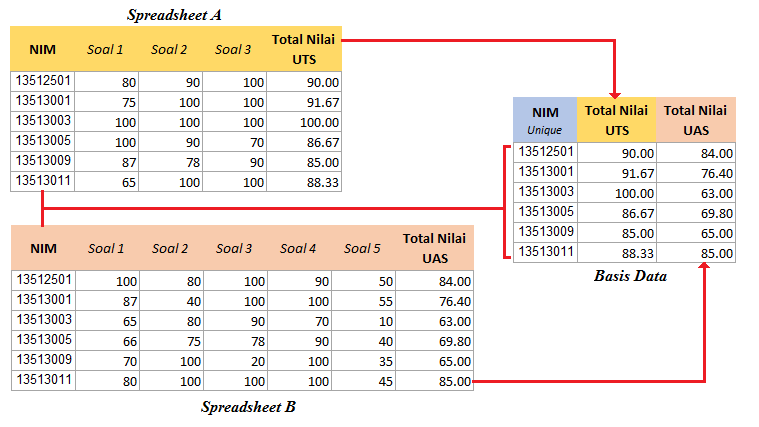
\includegraphics[width=0.9\textwidth]{resources/chapter-3-vertical-merge.png}
	    \caption{Contoh Penggabungan Vertikal}
		\label{VerticalMerge}
	\end{figure}

	Penggabungan secara vertikal membutuhkan suatu kolom \textit{key} dan unik yang dapat dijadikan patokan penggabungan data pada suatu baris data. Untuk masing-masing \textit{spreadsheet} yang akan digabungkan datanya, harus memiliki kolom \textit{key} dan unik yang sama dengan konteks data yang sama. Pada contoh pada gambar, kolom unik yang dipilih adalah kolom NIM. Penggabungan data dilakukan dengan mengambil data dari \textit{spreadsheet} A yakni data nilai UTS, dan dari \textit{spreadsheet} B yakni data nilai UAS, lalu dimasukkan ke dalam basis data pada tabel yang dipilih.

	\item Fragmen Horizontal dan Vertikal\\
	Fragmen gabungan ini terjadi ketika data yang digabungkan ada yang memiliki perbedaan kolom, ada juga yang tidak, atau juga dapat merupakan gabungan semua kolom yang ada. Contoh kasus yang dapat terjadi dapat dilihat pada Gambar \ref{BothTableMerge}.

	\begin{figure}[!htb]
	    \centering
	    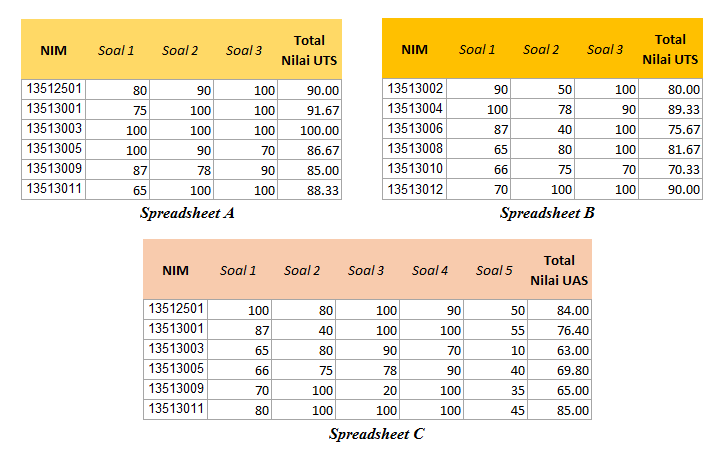
\includegraphics[width=0.9\textwidth]{resources/chapter-3-both-merge.png}
	    \caption{Contoh Tabel Penggabungan}
		\label{BothTableMerge}
	\end{figure}

	Terdapat tiga \textit{spreadsheet} dimana data pada \textit{spreadsheet} A dan \textit{spreadsheet} C memiliki jumlah kolom yang sama dan dapat digabung secara horizontal. Sedangkan, \textit{spreadsheet} A dan \textit{spreadsheet} B memiliki jumlah kolom yang berbeda namun kolom unik yang sama yakni NIM sehingga dapat digabungkan secara vertikal. Hasil penggabungan ketiga \textit{spreadsheet} ini akan menjadi tabel yang dapat dilihat pada Gambar \ref{BothMerge}.

	\begin{figure}[!htb]
	    \centering
	    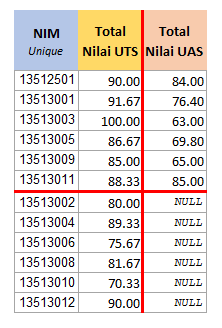
\includegraphics[width=0.3\textwidth]{resources/chapter-3-both-merge-db.png}
	    \caption{Contoh Penggabungan Horizontal dan Vertikal}
		\label{BothMerge}
	\end{figure}

	Karena dari hasil penggabungan data tidak semua kolom dapat dipenuhi, maka terdapat kolom yang berisikan NULL sebagai penanda bahwa kolom tersebut kosong dan tidak mendapatkan data dari \textit{spreadsheet}.
\end{enumerate}

\subsection{Interaksi Penyimpanan}
Penanganan interaksi penyimpanan menjadi penting pada saat terdapat dua atau lebih \textit{spreadsheet} memasukkan datanya pada suatu tabel yang sama. Kasus yang dapat terjadi adalah data yang telah sebelumnya dimasukkan oleh sebuah \textit{spreadsheet} dapat ditimpa oleh data dari \textit{spreadsheet} lainnya. Hal ini, jika memang tidak diharapkan, akan menyebabkan permasalahan kerusakan data. Pada kakas yang dibuat, diberikan penanganan berupa tombol pengecekan yang akan menjalankan fitur yang dapat melakukan pengecekan konflik data. Jika pengguna memang ingin melakukan penimpaan terhadap data yang sudah ada, maka peringatan dari fitur ini dapat diabaikan.

Urutan penyimpanan antar \textit{spreadsheet} tidak akan mempengaruhi hasil dengan syarat data yang disimpan dari kedua \textit{spreadsheet} merupakan data yang \textit{disjoint} atau kelompok data yang terpisah satu dengan yang lainnya. Jika syarat tersebut tidak dipenuhi, maka pengguna harus memasukkan data dengan urutan yang benar dan diperhitungkan agar data yang masuk sesuai dengan keinginan. Hal ini harus diperhitungkan dalam pengumpulan data yang dilakukan oleh pengguna.

\section{Analisis Alur Kerja Manusia dan Kakas} \label{Aluralur}
Pada subbab ini, akan dijelaskan perbedaan alur kerja manusia dalam pengumpulan data menggunakan aplikasi yang telah ditambahkan dengan kakas yang dibuat dengan aplikasi biasa. Selain itu, akan dijelaskan juga perubahan alur kakas di dalam menangani masukan pengguna.

\subsection{Alur Kerja Manusia}
Terdapat perbedaan alur kerja yang terjadi jika pengguna menggunakan aplikasi yang dibuat pada Tugas Akhir. Alur kerja lama dapat dilihat pada Gambar \ref{GambarWorkflowKerjaBiasa} dan alur kerja pada aplikasi \textit{spreadsheet} yang dibagun dapat dilihat pada Gambar \ref{GambarWorkflowKerja}.

\begin{figure}[!htb]
    \centering
    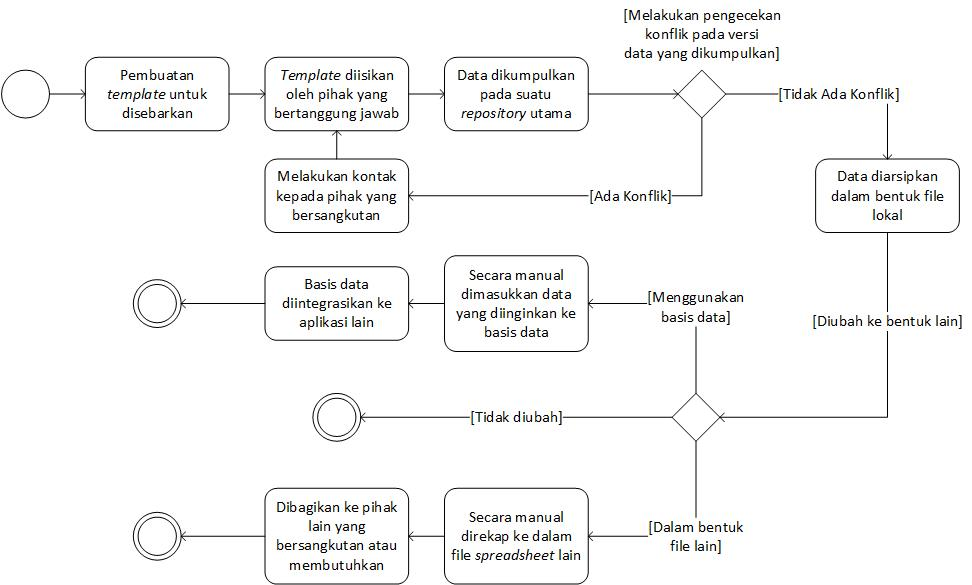
\includegraphics[width=1\textwidth]{resources/chapter-3-workflow-kerja-biasa.jpg}
    \caption{Alur Pengumpulan Data Biasa}
	\label{GambarWorkflowKerjaBiasa}
\end{figure}

\begin{figure}[htb]
    \centering
    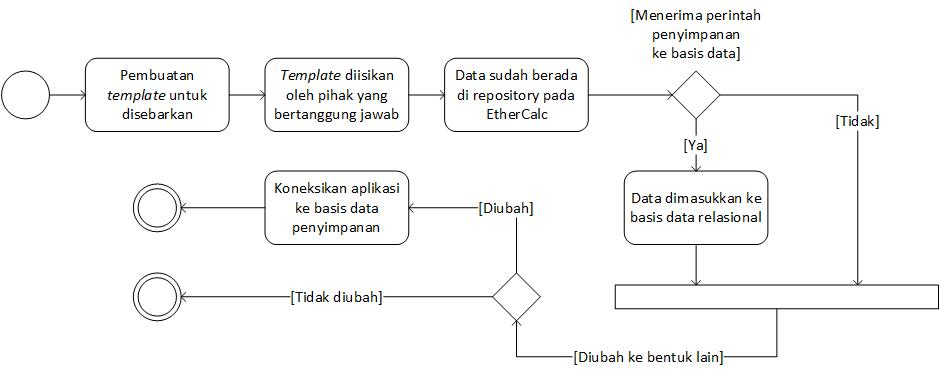
\includegraphics[width=1\textwidth]{resources/chapter-3-workflow-kerja.jpg}
    \caption{Alur Pengumpulan Data dengan Kakas yang Dibuat}
	\label{GambarWorkflowKerja}
\end{figure}

Seperti yang digambarkan pada alur tersebut, dengan menggunakan aplikasi dengan kakas yang dikembangkan akan mengurangi alur yang dibutuhkan untuk mengumpulkan data. Pengurangan alur terjadi pada bagian penanganan konflik pada versi-versi \textit{spreadsheet} yang berbeda dan menjadi hanya dibutuhkan satu cara untuk mengubah data ke bentuk lain, yakni menggunakan koneksi basis data.

\subsection{Alur Kerja Kakas}
Kakas yang dibuat akan mengubah alur aplikasi \textit{spreadsheet} yang umum dengan menambahkan mekanisme-mekanisme yang dibutuhkan. Alur aplikasi yang lama dapat dilihat pada Gambar \ref{GambarWorkflowBiasa} dan aplikasi \textit{spreadsheet} yang dibangun pada Tugas Akhir ini pada Gambar \ref{GambarWorkflow}.

\begin{figure}[htb]
    \centering
    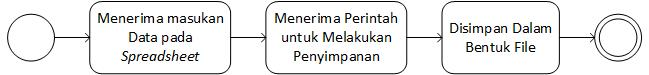
\includegraphics[width=0.7\textwidth]{resources/chapter-3-workflow-biasa.jpg}
    \caption{Alur Aplikasi \textit{Spreadsheet} Biasa}
	\label{GambarWorkflowBiasa}
\end{figure}

\begin{figure}[htb]
    \centering
    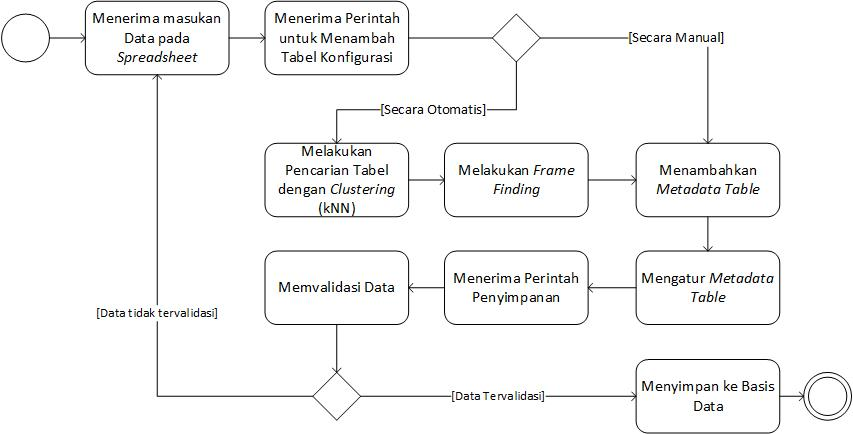
\includegraphics[width=1\textwidth]{resources/chapter-3-workflow.jpg}
    \caption{Alur Aplikasi \textit{Spreadsheet} dengan Kakas yang Dibuat}
	\label{GambarWorkflow}
\end{figure}

Dapat dilihat bahwa terdapat proses tambahan yang dilakukan pada aplikasi yang telah ditambahkan kakas yang dibuat pada Tugas Akhir ini. Proses tersebut terdiri dari pencarian bagian label dan data jika menggunakan pencarian otomatis, pengaturan \textit{metadata table} untuk aturan masukkan ke basis data, serta proses validasi. Fokus kakas ini hanya sampai menyimpan data pada basis data, sehingga permasalahan \textit{input} dan \textit{output} berupa \textit{file} tidak ditangani. Alur kolaborasi bukan merupakan fokus pengembangan kakas pada Tugas Akhir ini sehingga akan ditangani oleh aplikasi \textit{spreadsheet} yang dipilih.

% \section{Rencana Tindak Lanjut}
% Berdasarkan analisa yang telah dijelaskan pada bab-bab sebelumnya, pada Tugas Akhir ini akan dibangun aplikasi \textit{spreadsheet} dengan menggunakan EtherCalc sebagai teknologi utama. Pada Subbab \ref{TeknologiSpreadsheet} telah dijelaskan bahwa EtherCalc merupakan perangkat lunak \textit{spreadsheet} yang \textit{open source} dan memiliki kemampuan kolaborasi didalam penggunaannya. Sehingga dengan menggunakan EtherCalc, aspek-aspek yang telah dijelaskan pada Subbab \ref{AspekAplikasi} yang harus ada didalam pembangunan \textit{spreadsheet} ini sudah dapat dipenuhi. Pada Tugas Akhir ini akan dilakukan pengembangan dari EtherCalc yang berupa identifikasi label dan data, penanganan validasi data dan keterhubungannya dengan basis data relasional. Alur kerja dari aplikasi \textit{spreadsheet} yang akan dibuat dapat dilihat pada Gambar \ref{GambarWorkflow} pada Subbab \ref{AspekAplikasi}.
    \chapter{Rancangan, Implementasi, dan Pengujian}

\section{Perancangan Perangkat Lunak} \label{PerancanganPL}
Subbab perancangan perangkat lunak menjelaskan deskripsi aplikasi, analisis kebutuhan fungsional dan non-fungsional, desain perangkat lunak, serta interaksinya.

	\subsection{Deskripsi Umum Kakas}
	Kakas pengumpulan data yang dibuat merupakan pengembangan terhadap aplikasi \textit{spreadsheet} kolaboratif yang sudah ada sebelumnya yakni EtherCalc. Kakas yang ditambahkan ini yang akan melakukan pengaturan koneksi ke basis data. Saat pengguna menginginkan penyimpanan data ke dalam basis data yang dituju, kakas ini akan melakukan pencarian bagian label dan data dan melakukan validasi masukan sebelum memasukkan data ke dalam basis data. 

	\subsection{Spesifikasi Kebutuhan}
	Pada subbab ini akan dipaparkan \textit{use case} kakas yang akan dibuat serta kebutuhan fungsional dan non-fungsional dari kakas. Kasus penggunaan oleh pengguna diberi ID dengan format UC-XX dengan UC menyatakan \textit{use case} dan XX menyatakan nomor. Pengguna adalah pihak yang menggunakan aplikasi \textit{spreadsheet} yang sudah ditambahkan kakas pengumpulan data. Kasus penggunaan oleh pengguna dijelaskan pada Tabel \ref{KebutuhanPengguna}.

	\begin{small}
	\begin{longtable}{ | p{2cm} | p{10cm} | }
	    \caption{Kasus Penggunaan oleh Pengguna}
	    \label{KebutuhanPengguna}\\ \hline
	    \centering\bfseries{ID} & \centering\bfseries{Deskripsi} \tabularnewline \hline
	    \endfirsthead
	    \hline
	    \centering\bfseries{ID} & \centering\bfseries{Deskripsi} \tabularnewline \hline
	    \endhead
	    UC-01 & Pengguna dapat menentukan basis data tujuan dengan konfigurasi basis data yang diinginkan. \\ \hline
	    UC-02 & Pengguna dapat menyimpan data yang dikumpulkan ke dalam basis data pada saat dibutuhkan. \\ \hline
	    UC-03 & Pengguna dapat mendefinisikan \textit{metadata table} yang ingin disimpan secara manual maupun otomatis oleh kakas. \\ \hline
	    UC-04 & Pengguna dapat mengubah metadata pada \textit{metadata table} yang ingin disimpan. \\ \hline
	    UC-05 & Pengguna dapat mendefinisikan aturan validasi data. \\ \hline
	    UC-06 & Pengguna dapat mengunggah berkas \textit{spreadsheet} ke dalam aplikasi. \\ \hline
	\end{longtable}
	\end{small}

	Untuk \textit{use case} dengan kode UC-06, sudah ditangani oleh aplikasi \textit{EtherCalc} sehingga tidak akan ditangani oleh kakas yang akan dikembangkan. Berdasarkan kasus penggunaan di atas, dirancang kebutuhan fungsional perangkat lunak yang diberi ID dengan format FR-XX dengan FR merupakan singkatan dari \textit{functional requirement} dan XX menyatakan nomor kebutuhan. Kebutuhan fungsional dijelaskan pada Tabel \ref{KebutuhanFungsional}.

	\begin{small}
	\begin{longtable}{ | p{2cm} | p{6cm} | p{4cm} | }
	    \caption{Kebutuhan Fungsional Kakas}
	    \label{KebutuhanFungsional}\\ \hline
	    \centering\bfseries{ID} & \centering\bfseries{Deskripsi} & \centering\bfseries{ID Use Case Terkait} \tabularnewline \hline
	    \endfirsthead
	    \hline
	    \centering\bfseries{ID} & \centering\bfseries{Deskripsi} & \centering\bfseries{ID Use Case Terkait} \tabularnewline \hline
	    \endhead
	    FR-01 & Kakas dapat melakukan koneksi kepada basis data yang ditentukan oleh pengguna melalui data masukan berupa \textit{host}, \textit{port}, \textit{username}, \textit{password}, dan \textit{database} dari basis data yang dituju. & UC-01 \\ \hline
	    FR-02 & Kakas dapat melakukan perintah basis data kepada basis data yang dituju. & UC-01, UC-02 \\ \hline
	    FR-03 & Kakas menyediakan fitur untuk dapat melakukan penyimpanan data saat pengguna ingin melakukan penyimpanan. & UC-02 \\ \hline
	    FR-04 & Kakas menyediakan fitur menambah dan mengurangi \textit{metadata table} baik secara pendeteksian otomatis maupun manual. & UC-03 \\ \hline
	    FR-05 & Kakas dapat menampilkan hasil identifikasi label dan data dalam bentuk \textit{metadata table}. & UC-03, UC-04 \\ \hline
	    FR-06 & Kakas menyediakan fitur bagi pengguna agar dapat mengubah hasil identifikasi label dan data. & UC-04 \\ \hline
	    FR-07 & Kakas menyediakan fitur bagi pengguna agar dapat menambahkan dan mengubah batasan masukan pada suatu data. & UC-05 \\ \hline
	    FR-08 & Kakas dapat melakukan validasi data masukan sesuai dengan batasan yang diberikan oleh pengguna. & UC-05 \\ \hline
	    FR-09 & Kakas dapat memberitahukan kesalahan validasi yang terjadi. & UC-05 \\ \hline
	\end{longtable}
	\end{small}

	Selain kebutuhan fungsional, dijabarkan juga kebutuhan non-fungsional yang memiliki ID dengan format NF-XX dengan NF merupakan singkatan dari \textit{non-functional requrirement} dan XX menyatakan nomor. Kebutuhan non-fungsional disajikan pada Tabel \ref{KebutuhanNonfungsional}.

	\begin{small}
	\begin{longtable}{ | p{2cm} | p{6cm} | p{4cm} | }
	    \caption{Kebutuhan Non-fungsional Kakas}
	    \label{KebutuhanNonfungsional}\\ \hline
	    \centering\bfseries{ID} & \centering\bfseries{Deskripsi} & \centering\bfseries{ID Use Case Terkait} \tabularnewline \hline
	    \endfirsthead
	    \hline
	    \centering\bfseries{ID} & \centering\bfseries{Deskripsi} & \centering\bfseries{ID Use Case Terkait} \tabularnewline \hline
	    \endhead
	    NF-01 & Data masukan pengguna disimpan secara persisten. & UC-01, UC-02 \\ \hline
	    NF-02 & Kakas dapat berjalan di atas aplikasi \textit{spreadsheet} EtherCalc. & - \\ \hline
	\end{longtable}
	\end{small}

	\subsection{Kebutuhan Modul} \label{KebutuhanModul}
	Pembangunan fitur ini di atas aplikasi EtherCalc terdiri dari lima buah modul, yaitu:
	\begin{enumerate}
		\item Modul \texttt{player}, bertugas sebagai jembatan antara \textit{front-end} dan \textit{back-end} dari fitur.
		\item Modul \texttt{mysql}, bertugas untuk antarmuka baca tulis basis data.
		\item Modul \texttt{framefinder}, bertugas untuk mendeteksi secara otomatis bagian label dan data pada tabel.
		\item Modul \texttt{hierarchyfinder}, bertugas untuk mendeteksi secara otomatis tabel-tabel yang ada dalam suatu \textit{sheet}.
		\item Modul \texttt{table}, bertugas untuk mengelola \textit{metadata table}, melakukan validasi data, dan membuat representasi relasional.
	\end{enumerate}

	Ketergantungan antar modul dapat dilihat pada Gambar \ref{ModuleDependency}

	\begin{figure}[htb]
	    \centering
	    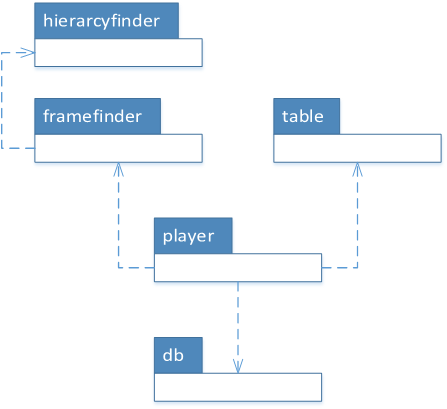
\includegraphics[width=0.4\textwidth]{resources/chapter-4-module-dependecy.png}
	    \caption{Ketergantungan Antar Modul}
		\label{ModuleDependency}
	\end{figure}

	\subsection{Kolaborasi Antar Modul}
	Proses fitur ini akan dilakukan melalui modul \texttt{player} yang dapat menerima perintah pengguna melalui \textit{front-end}. Selanjutnya modul \texttt{framefinder} akan melakukan pendeteksian label dan data secara otomatis pada masing-masing tabel yang terdapat pada \textit{sheet}. Tabel-tabel tersebut didapatkan melalui modul \texttt{hierarchyfinder}. Selanjutnya, pada saat menerima perintah penyimpanan, modul \texttt{table} akan dipanggil oleh \texttt{player}. Jika data masukan sudah benar, maka modul \texttt{mysql} akan melakukan pennyimpanan ke dalam basis data. Kolaborasi antar modul disajikan pada Gambar \ref{ModuleFlow}.

	\begin{figure}[htb]
	    \centering
	    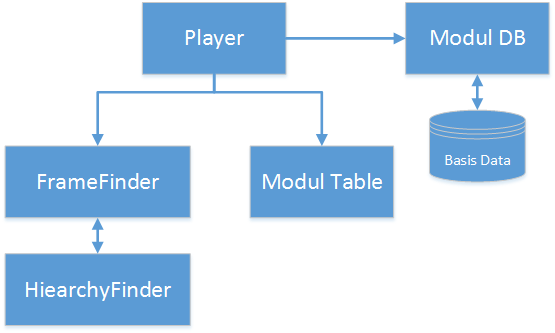
\includegraphics[width=0.5\textwidth]{resources/chapter-4-module-flow.png}
	    \caption{Kolaborasi Antar Modul}
		\label{ModuleFlow}
	\end{figure}

	Pada aplikasi Ethercalc, modul yang ditambahkan akan berada di bawah modul \texttt{player} yang sudah ada. Ilustrasi penempatan modul yang dibuat pada aplikasi EtherCalc yang sudah ada dapat dilihat pada Gambar \ref{ModulePlacing}.

	\begin{figure}[htb]
	    \centering
	    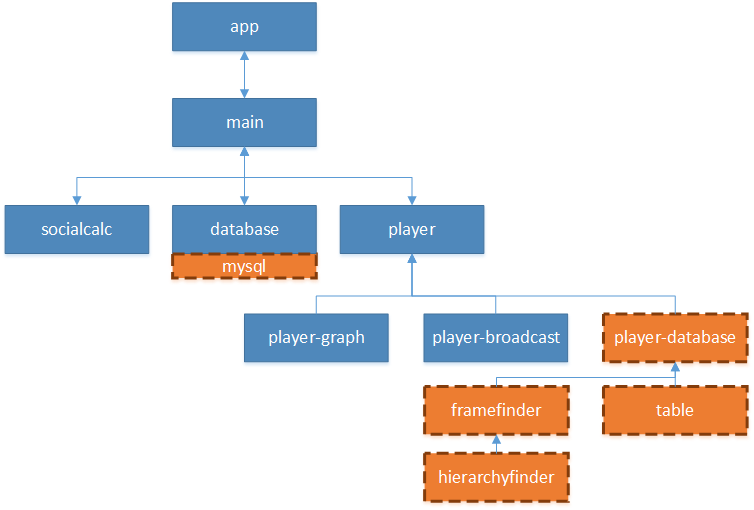
\includegraphics[width=0.6\textwidth]{resources/chapter-4-module-placing.png}
	    \caption{Interaksi dengan Modul yang Sudah Ada}
		\label{ModulePlacing}
	\end{figure}

	\subsection{Arsitektur}
	Aplikasi dibuat dengan menggunakan bantuan Docker sehingga diharapkan dapat dengan mudah dipasang pada berbagai \textit{platform}. Aplikasi terdiri dari tiga \textit{docker container} yakni untuk aplikasi utama, basis data redis, dan basis data MySQL. \textit{File} \texttt{docker-compose.yml} yang dibuat untuk mendefinisikan \textit{docker container} yang digunakan dapat dilihat pada Kode \ref{KodeCompose}

	\begin{lstlisting}[frame=single, basicstyle=\linespread{1}\scriptsize\listingsfont, captionpos=b, caption={Kode pada docker-compose.yml}, label=KodeCompose]
	ethercalc:
	  build: .
	  ports:
	    - "80:8000"
	  links:
	    - redis:redis
	    - mysql:mysql
	  restart: always
	redis:
	  image: redis:latest
	  volumes:
	    - /var/lib/redis:/data
	  command: redis-server --appendonly yes
	  restart: always
	mysql:
	  image: mysql:5.7
	  volumes:
	    - db_data:/var/lib/mysql
	  restart: always
	  environment:
	    MYSQL_ROOT_PASSWORD: root
	    MYSQL_DATABASE: TA
	    MYSQL_USER: user
	    MYSQL_PASSWORD: user
	\end{lstlisting}

	Untuk menyimpan \textit{state} konfigurasi tabel dan \textit{mapping} \textit{metadata table} dengan data pada basis data, digunakan dua tabel basis data yang sudah didefinisikan sebelumnya. Kedua tabel basis data ini dinamakan s\_database\_state dan s\_database\_wlog, kedua tabel ini tidak memiliki keterhubungan. Atribut yang terdapat pada kedua tabel ini dapat dilihat pada diagram struktur basis data pada Gambar \ref{StructureDiagram}.

	\begin{figure}[htb]
	    \centering
	    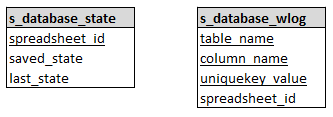
\includegraphics[width=0.5\textwidth]{resources/chapter-4-architect-db.png}
	    \caption{Diagram Struktur Tabel Penyimpanan Konfigurasi}
		\label{StructureDiagram}
	\end{figure}

	\textit{metadata table} yang ditampilkan kepada pengguna akan berasal dari tabel s\_database\_state dan juga disimpan pada tabel tersebut. Kegunaan  s\_database\_wlog adalah mencatat pemetaan data kepada \textit{metadata table} sehingga saat \textit{metadata table} dihapus, data yang berasal dari \textit{metadata table} tersebut dapat juga dihapus.

	Kakas dibuat di atas aplikasi EtherCalc, sehingga akan diimplementasi tambahan modul maupun menggunakan modul yang sudah ada pada EtherCalc. Interaksi antar modul yang dibuat dengan modul yang sudah ada serta dengan data masukan dapat dilihat pada Gambar \ref{ArchDiagram}.

	\begin{figure}[htb]
	    \centering
	    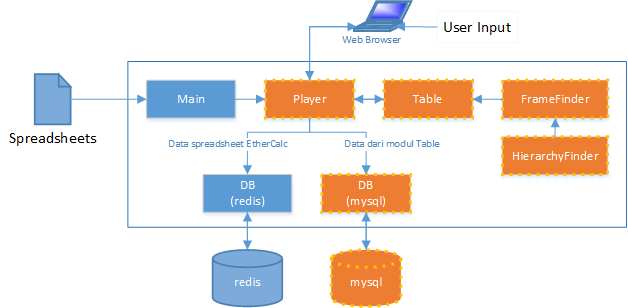
\includegraphics[width=0.7\textwidth]{resources/chapter-4-architecture.png}
	    \caption{Diagram Arsitektur Aplikasi}
		\label{ArchDiagram}
	\end{figure}

	Pada diagram arsitektur terlihat bahwa masih terdapat dua basis data yakni redis dan MySQL. Hal ini dilakukan agar data mengenai format dan cara ditampilkan pada aplikasi EtherCalc tetap disimpan pada basis data redis sedangkan data yang ingin dikumpulkan dan digabungkan oleh pengguna dimasukkan pada basis data relasional MySQL.

	% Modul-modul dan fitur dibuat di atas aplikasi EtherCalc, sehingga arsitektur kakas akan mengikuti arsitektur aplikasi EtherCalc yang telah dijelaskan pada Subbab \ref{TeknologiSpreadsheet}.

\section{Implementasi}
Implementasi dilakukan dengan membangun modul yang telah dijabarkan pada Subbab \ref{KebutuhanModul} dengan menggunakan bahasa Javascript, menyesuaikan dengan modul lain yang telah ada pada aplikasi EtherCalc. Pada bagian ini akan dijelaskan antarmuka dan modul-modul yang diimplementasikan.
	\subsection{Antarmuka}
	Antarmuka aplikasi pada Tugas Akhir ini mengikuti antarmuka yang telah ada sebelumnya pada aplikasi EtherCalc. Fitur baru yang ditambahkan akan menempati menu baru pada bagian atas antarmuka dengan nama `Data Collector`. Antarmuka awal dapat dilihat pada Gambar \ref{Antarmuka1}.

	\begin{figure}[htb]
	    \centering
	    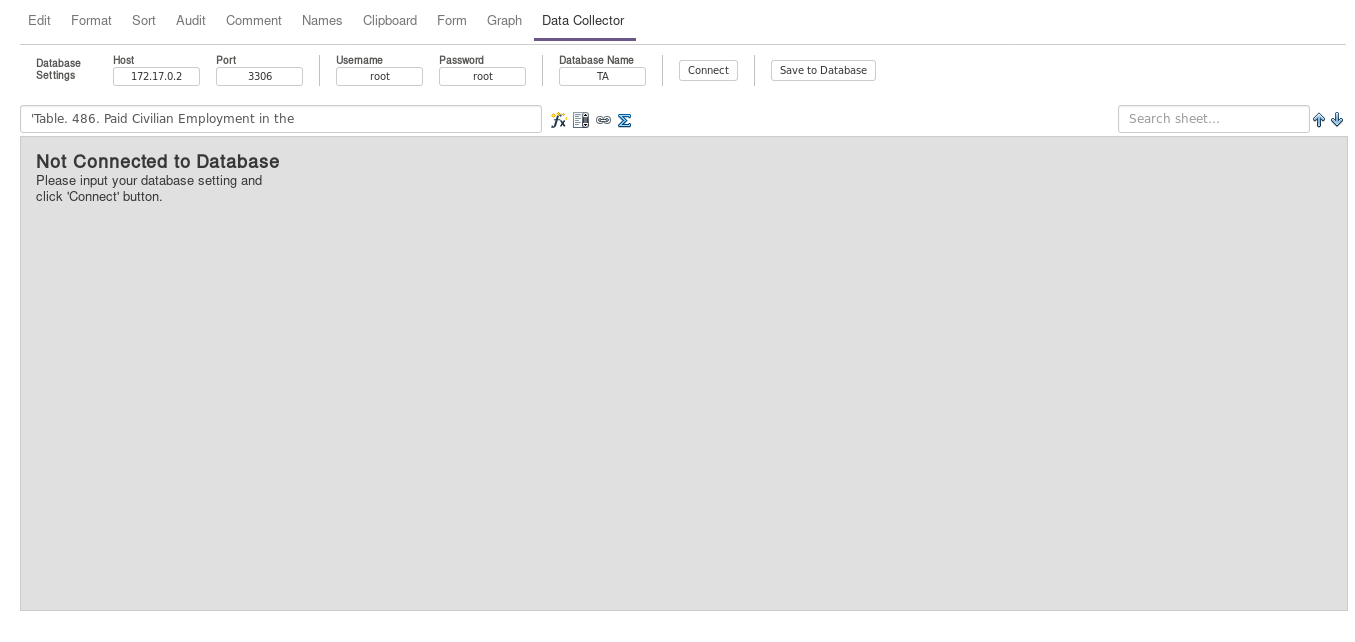
\includegraphics[width=1.0\textwidth]{resources/chapter-4-interface-1.png}
	    \caption{Antarmuka Awal}
		\label{Antarmuka1}
	\end{figure}

	Terdapat dua bagian utama pada antarmuka ini, yang pertama adalah area pengaturan basis data dimana pengguna bisa dapat mengatur koneksi ke basis data yang diinginkan. Yang kedua adalah area tempat \textit{metadata table} dapat ditambahkan dan dikurangi berdasarkan masukan pengguna. Pada bagian kiri area \textit{metadata table}, terdapat dua pilihan metode untuk membuat \textit{metadata table} yakni secara manual maupun otomatis. Kedua area ini dapat dilihat pada Gambar \ref{Antarmuka2}.

	\begin{figure}[htbp]
	    \centering
	    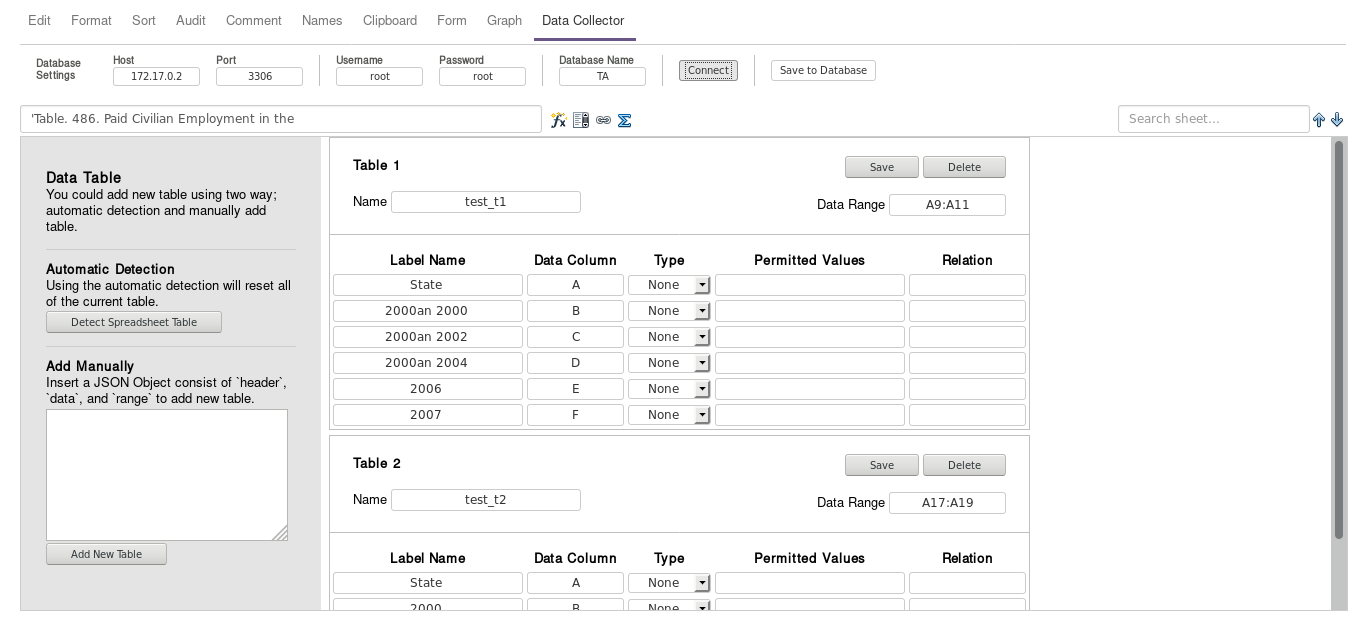
\includegraphics[width=1.0\textwidth]{resources/chapter-4-interface-2.png}
	    \caption{Antarmuka \textit{metadata table}}
		\label{Antarmuka2}
	\end{figure}

	Pada bagian \textit{metadata table}, pengguna dapat menentukan nama label, tipe data, nilai-nilai yang diizinkan, dan relasinya terhadap kumpulan sel lain untuk suatu kolom data. Pengguna dapat juga mengubah nama tabel tujuan ke basis data serta menghapus \textit{metadata table}. Jika terjadi kesalahan pada saat validasi, pengguna akan diberikan pesan kesalahan dan diharapkan untuk memperbaiki data pada sel yang dianggap memiliki kesalahan. Interaksi ini dapat dilihat pada Gambar \ref{Antarmuka3}.

	\begin{figure}[htbp]
	    \centering
	    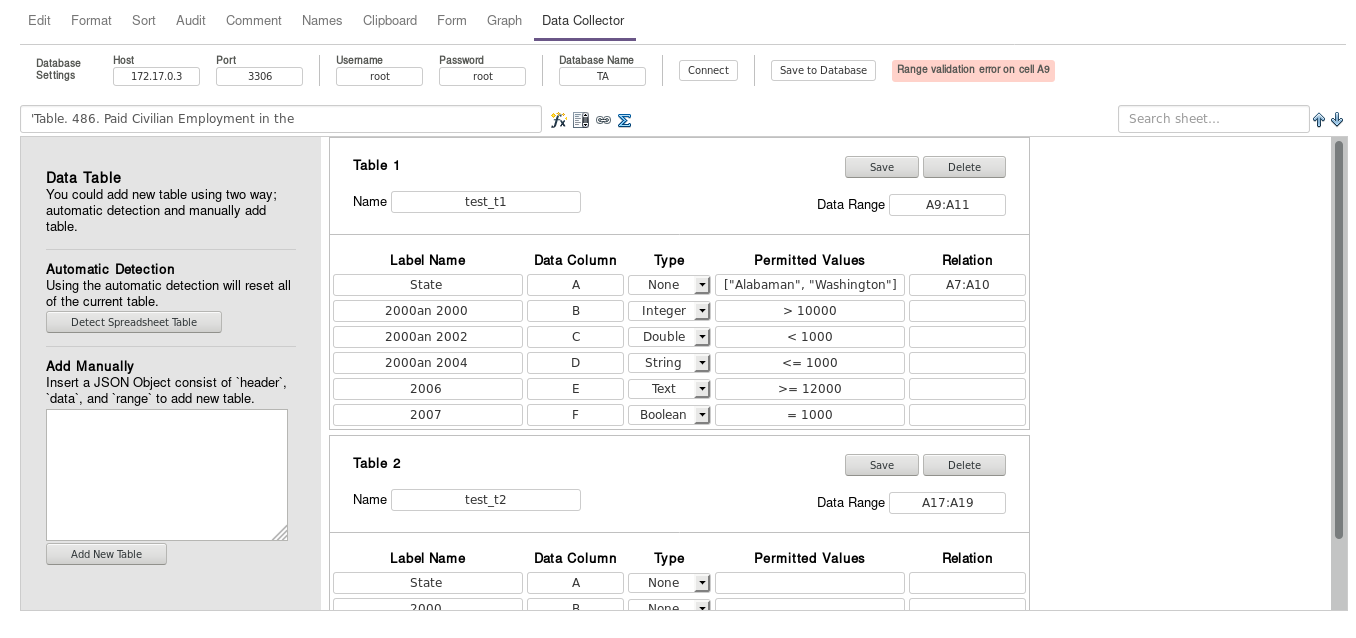
\includegraphics[width=1.0\textwidth]{resources/chapter-4-interface-3a.png}
	    \caption{Antarmuka Perubahan \textit{metadata table}}
		\label{Antarmuka3}
	\end{figure}
	
	\subsection{Modul Main}
	Modul \texttt{Main} merupakan modul yang sudah ada pada aplikasi EtherCalc. Untuk mengimplementasi kakas, modul ini dikembangkan lagi dengan menambahkan beberapa \textit{endpoint} API yang dibutuhkan. Seluruh API ini akan dipanggil melalui modul \texttt{Player}. API yang ditambahkan pada Tugas Akhir ini adalah:
	\begin{enumerate}
		\item \texttt{POST /\_database/connect} \\
		Digunakan untuk melakukan pengecekan koneksi ke basis data. Parameter yang dibutuhkan adalah:
		\begin{itemize} 
			\item host: \textit{host} basis data.
			\item port: \textit{port} basis data.
			\item user: \textit{user} basis dat yang digunakan.
			\item password: \textit{password} untuk \textit{user} yang digunakan.
			\item database: nama \textit{database} yang digunakan.
		\end{itemize}
	
		\item \texttt{POST /\_database/state} \\
		Digunakan untuk melakukan penyimpanan \textit{state} \textit{metadata table}. Parameter yang dibutuhkan adalah:
		\begin{itemize} 
			\item tables: data \textit{metadata table} dalam bentuk JSON.
			\item setting: pengaturan koneksi ke basis data yang dipilih berupa JSON Object.
		\end{itemize}

		\item \texttt{POST /\_database/state/[spreadsheet\_id]} \\
		Digunakan untuk mendapatkan data \textit{state} \textit{metadata table} pada suatu \textit{spreadsheet}. Parameter yang dibutuhkan adalah::
		\begin{itemize}
			\item setting: pengaturan koneksi ke basis data yang dipilih berupa JSON Object.
		\end{itemize}

		\item \texttt{POST /\_database/create} \\
		Digunakan untuk melakukan penyimpanan data yang telah dikumpulkan sesuai dengan aturan pada \textit{metadata table}. Parameter yang dibutuhkan adalah:
		\begin{itemize} 
			\item table: data dari \textit{metadata table} yang telah diubah menjadi bentuk relasional dalam bentuk JSON.
			\item setting: pengaturan koneksi ke basis data yang dipilih berupa JSON Object.
		\end{itemize}
	
		\item \texttt{GET /\_framefinder/[spreadsheet\_id]/[start\_col]/[end\_col]\\/[start\_row]/[end\_row]} \\
		Digunakan untuk mendapatkan hasil pencarian label dan data diantara kolom dan baris tertentu.

		\item \texttt{GET /\_hierarchical/[spreadsheet\_id]} \\
		Digunakan untuk mendapatkan perkiraan kelompok sel yang merupakan suatu kesatuan tabel.	
	\end{enumerate}

	\subsection{Modul Player}
	Modul \texttt{player} merupakan modul yang menjembatani masukan pengguna dari yang berasal dari \textit{front-end} sehingga dapat diterima oleh modul yang berada di \textit{back-end}. Modul ini hanya terdiri dari satu kelas utama yakni kelas \texttt{player} yang berisi fungsi-fungsi yang dapat dipanggil oleh \textit{front-end} yang dapat dilihat pada Lampiran A.
	
	\subsection{Modul DB}
	Modul basis data digunakan sebagai antarmuka modul lain untuk melakukan operasi I/O basis data. Pada Tugas Akhir ini, basis data yang digunakan adalah MySQL. Modul ini hanya terdiri dari satu kelas utama yakni kelas \texttt{mysql}. Kelas ini memiliki tugas sebagai penghubung kakas ke basis data MySQL yang dipilih. Fungsi-fungsi yang terdapat pada kelas ini dapat dilihat pada Lampiran A.

	Tabel akan dibuat pada basis data yang ditentukan, setiap tabel merepresentasikan suatu tabel pada \textit{spreadsheet} yang ditentukan oleh pengguna. \textit{Header} yang didefinisikan oleh pengguna pada \textit{spreadsheet} akan dijadikan \textit{column} pada tabel basis data, tipe yang dibentuk mengikuti masukan pengguna. Tiap baris data yang ada dibawah \textit{header} pada \textit{spreadsheet} akan ditranslasikan menjadi bentuk relasional agar dapat dimasukan ke dalam tabel.
	
	\subsection{Modul Hierarchyfinder}
	Modul \texttt{hierarchyfinder} menggunakan algoritma kNN jenis \textit{hierarchical clustering} untuk dapat mengetahui mana yang merupakan suatu kesatuan tabel pada suatu \textit{sheet}. Modul ini dapat menentukan tabel-tabel yang terdapat pada suatu \textit{sheet} yang selanjutnya akan dilakukan identifikasi label oleh modul \texttt{framefinder}. Algoritma \textit{hierarchical clustering} yang digunakan menganggap setiap sel pada \textit{spreadsheet} merupakan suatu node. Sel-sel yang bersebelahan dengan sel tersebut akan dianggap tetangga sehingga memiliki jarak sama dengan 0. Sel yang digabungkan dengan sel lain akan dihitung sebagai satu \textit{node}. Aturan perhitungan jarak antar \textit{node} dapat dilihat pada kode di Kode \ref{KodeJarak}.\\

	\begin{lstlisting}[frame=single, basicstyle=\linespread{1}\scriptsize\listingsfont, captionpos=b, caption={Perhitungan Jarak \textit{Node}}, label=KodeJarak]
	# Fungsi cellDistance(v1, v2)
	# Parameter pada fungsi adalah v1 (node 1) dan v2 (node 2)
	t = new Table null, null
	colD = t.GetCellCol(v1[0]) - t.GetCellCol(v2[0])
	rowD = t.GetCellRow(v1[0]) - t.GetCellRow(v2[0])

	# Jika sel saling bertetangga tetapi bukan secara diagonal
	# Jika bertetangga, jarak kedua sel adalah 0
	if colD == 0
		if rowD == 1 or rowD == -1
			return 0
	if rowD == 0
		if colD == 1 or colD == -1
			return 0

	# Jika tidak, cek apakah sel bertetangga secara diagonal
	# Jika bertetangga, jarak kedua sel adalah 0
	leftTop = [[v1[1], v1[2]], [v2[1], v2[2]]]
	leftBot = [[v1[1], (v1[2] + v1[4])], [v2[1], (v2[2] + v2[4])]]
	righTop = [[(v1[1] + v1[3]), v1[2]], [(v2[1] + v2[3]), v2[2]]]
	righBot = [[(v1[1] + v1[3]), (v1[2] + v1[4])], [(v2[1] + v2[3]), (v2[2] + v2[4])]]

	if (leftTop[0][0] == righTop[1][0] and leftTop[0][1] == righTop[1][1])
		return 0
	if (leftBot[0][0] == righBot[1][0] and leftBot[0][1] == righBot[1][1])
		return 0

	if (leftTop[1][0] == righTop[0][0] and leftTop[1][1] == righTop[0][1])
		return 0
	if (leftBot[1][0] == righBot[0][0] and leftBot[1][1] == righBot[0][1])
		return 0

	if (leftTop[0][0] == leftBot[1][0] and leftTop[0][1] == leftBot[1][1])
		return 0
	if (righTop[0][0] == righBot[1][0] and righTop[0][1] == righBot[1][1])
		return 0

	if (leftTop[1][0] == leftBot[0][0] and leftTop[1][1] == leftBot[0][1])
		return 0
	if (righTop[1][0] == righBot[0][0] and righTop[1][1] == righBot[0][1])
		return 0

	# Jika tidak juga, hitung jarak menggunakan teknik Euclidian
	dist = Math.sqrt(Math.pow((v2[1] + (v2[3]/2)) - (v1[1] + (v1[3]/2)), 2) + Math.pow((v2[2] + (v2[4]/2)) - (v1[2] + (v1[4]/2)), 2));
	return dist
	\end{lstlisting}

	Hasil dari pengelompokan ini berupa kelompok-kelompok tabel pada \textit{spreadsheet}. Setiap tabel yang teridentifikasi selanjutnya akan dicari bagian \textit{header} dan \textit{label} menggunakan modul \texttt{framefinder}.

	\subsection{Modul Framefinder}
	Modul \texttt{framefinder} melakukan pengidentifikasian terhadap tabel yang ada sehingga dapat diketahui baris yang merupakan \textit{header} dan \textit{data}. Implementasi modul ini dilakukan dengan mengikuti implementasi yang dilakukan pada penelitian yang dilakukan oleh Chen \citep{Chen2013}. Modul ini terdiri dari 5 kelas yang dapat dilihat pada Lampiran A.

	\begin{enumerate}
		\item Kelas LoadSheet\\
		Kelas ini melakukan pengambilan data pada \textit{spreadsheet} dengan cara membaca file \textit{spreadsheet} dan membentuk representasi kelas yang dibutuhkan. Kelas ini memiliki satu atribut utama yakni cmysheet yang merupakan kelas MySheet. Fungsi-fungsi yang terdapat pada kelas ini dapat dilihat pada Lampiran A.

		\item Kelas MySheet\\
		Kelas MySheet merupakan kelas yang merepresentasikan \textit{sheet} pada \textit{spreadsheet} yang dipilih. Kelas ini memiliki 4 atribut yang dapat dilihat pada Lampiran A. Pada kelas ini terdapat 3 fungsi yang dapat dilihat juga pada Lampiran A.

		\item Kelas MyCell\\
		Kelas MyCell merupakan kelas yang merepresentasikan sel pada suatu \textit{sheet}. Kelas ini memiliki 17 atribut yang dapat dilihat pada Lampiran A.
	\end{enumerate}

	% Pada kelas ini terdapat 3 fungsi yang dapat dilihat pada Tabel \ref{FungsiMyCell}.

	% \begin{small}
	% \begin{longtable}{ | p{4cm} | p{9cm} | }
	%     \caption{Fungsi pada Kelas MyCell}
	%     \label{FungsiMyCell}\\ \hline
	%     \centering\bfseries{Nama Fungsi} & \centering\bfseries{Deskripsi} \tabularnewline \hline
	%     \endfirsthead
	%     \hline
	%     \centering\bfseries{Nama Fungsi} & \centering\bfseries{Deskripsi} \tabularnewline \hline
	%     \endhead
	%     writestrAlignstyle & Mendapatkan representasi \textit{string} untuk \textit{align} pada sel. Digunakan pada saat penulisan ke dalam file untuk dibaca pada algoritma CRF.\\ \hline
	%     writestrBorderstyle & Mendapatkan representasi \textit{string} untuk \textit{border} pada sel. Digunakan pada saat penulisan ke dalam file untuk dibaca pada algoritma CRF.\\ \hline
	%     getIndents & Digunakan untuk menentukan nilai atribut indentasi dengan menghitung seberapa dalam indentasi pada konten.\\ \hline
	% \end{longtable}
	% \end{small}

	\subsubsection{Kelas FeatureSheetRow}
	Kelas ini bertugas untuk melakukan ekstraksi fitur pada tiap baris sel yang telah dikumpulkan dari \textit{spreadsheet}. Fitur-fitur yang diambil untuk setiap barisnya dapat dilihat pada Lampiran A.

	Fitur-fitur di atas mengikuti fitur yang didefinisikan pada penelitian yang dilakukan oleh Chen \citep{Chen2013}. Fitur-fitur ini akan digunakan dalam perhitungan algoritma CRF.

	\subsubsection{Kelas PredictSheetRows}
	Kelas PredictSheetRows memiliki tugas untuk melakukan konversi fitur-fitur yang telah didapatkan pada kelas FeatureSheetRow menjadi bentuk file teks yang dapat dibaca oleh program CRFPP yang akan menjalankan algoritma CRF pada file tersebut. Contoh file yang dihasilkan oleh kelas ini dapat dilihat pada Kode \ref{KodeFile}.\\

	\begin{lstlisting}[frame=single, basicstyle=\linespread{1}\scriptsize\listingsfont, captionpos=b, caption={File Berisikan Fitur Tiap Baris}, label=KodeFile]
	DeadlineTA.xls____Sheet1____1 1 0 1 0 0 1 0 1 0 0 0 0 0 0 1 0 1 1 0 0 0 0 0 Header
	DeadlineTA.xls____Sheet1____2 0 1 1 0 0 1 0 0 0 0 0 1 0 0 1 0 1 1 0 0 0 0 0 Data
	DeadlineTA.xls____Sheet1____3 0 1 1 0 0 1 0 0 0 0 0 1 0 0 1 0 0 0 0 0 0 0 0 Data
	DeadlineTA.xls____Sheet1____4 0 1 1 0 0 1 0 0 0 0 0 1 0 0 1 0 0 0 0 0 0 0 0 Data
	DeadlineTA.xls____Sheet1____5 0 1 1 0 0 1 0 0 0 0 0 1 0 0 1 0 0 1 0 0 0 0 0 Data
	\end{lstlisting}

	File tersebut ditulis dalam format \texttt{namafile\_namasheet\_bariske [fitur-fitur pada baris] label}. File ini yang akan diolah oleh algoritma dan digunakan untuk memprediksi label dari setiap baris tersebut. Algoritma yang digunakan adalah Conditional Random Field dan menggunakan aplikasi CRFPP yang berjalan eksternal diluar kelas ini untuk membaca file, membaca model, serta memprediski label.

	\subsection{Modul Table}
	Modul \texttt{table} memiliki tugas untuk mengelola tampilan dan isi \textit{metadata table}, melakukan validasi data masukan, dan membuat representasi relasional yang dapat diterima oleh basis data. Modul \texttt{table} hanya memiliki satu kelas yakni kelas \texttt{table}. Kelas ini memiliki 8 atribut yang dapat dilihat pada Lampiran A.	Pada kelas ini terdapat 6 fungsi yang dapat dilihat pada Lampiran A.

	Modul ini berinteraksi langsung dengan modul \texttt{player} pada saat akan melakukan penyimpanan \textit{state} \textit{metadata table} dan menampilkan \textit{metadata table} pada \textit{front-end}. Selain itu, modul ini juga berhubungan dengan modul \texttt{mysql} pada saat melakukan penyimpanan.

\section{Pengujian}
Pengujian dilakukan hanya kepada fitur yang di buat pada Tugas Akhir ini dan tidak kepada aplikasi EtherCalc secara keseluruhan. Pada subbab ini akan dibahas kasus-kasus yang diuji dan hasil dari pengujian tersebut.

	\subsection{Tujuan Pengujian}
	Pada fitur yang dibangun pada Tugas Akhir ini, pengujian yang dilakukan mempunyai tujuan yaitu fitur yang diimplementasi dapat berjalan dengan baik. Pengujian yang dilakukan akan dikaitkan pada kebutuhan-kebutuhan kakas yang telah didefinisikan sebelumnya. Dari pengujian akan dilihat kesesuaian hasil sesungguhnya dengan hasil yang diinginkan.

	% \begin{enumerate}
	% 	\item Fitur yang diimplementasi dapat berjalan dengan baik. Pengujian yang dilakukan akan dikaitkan pada kasus-kasus penggunaan yang dapat terjadi. Dari pengujian akan dilihat kesesuaian hasil sesungguhnya dengan hasil yang diinginkan.
	% 	\item Mencatat waktu eksekusi yang dibutuhkan untuk fitur-fitur yang ditambahkan.
	% \end{enumerate}

	\subsection{Lingkungan Pengujian}
	Pengujian dilakukan pada komputer dengan spesifikasi pada Tabel \ref{LingPengujian}.

	\begin{small}
	\begin{longtable}{ | p{3cm} | p{9cm} | }
	    \caption{Spesifikasi Lingkungan Pengujian}
	    \label{LingPengujian}\\ \hline
	    \centering\bfseries{Komponen} & \centering\bfseries{Deskripsi} \tabularnewline \hline
	    \endfirsthead
	    \hline
	    \centering\bfseries{Komponen} & \centering\bfseries{Deskripsi} \tabularnewline \hline
	    \endhead
		Prosesor & AMD A8-4500M APU with Radeon(tm) HD Graphics 1.90GHz\\ \hline
		Memori Fisik & 12 GB\\ \hline
		\textit{Storage} & 50 GB\\ \hline
		Sistem Operasi & Arch Linux 64-bit\\ \hline
		Docker version & 1.13.1\\ \hline
		\textit{Web browser} & Mozilla Firefox 51.0.1\\ \hline
	\end{longtable}
	\end{small}

	\subsection{Eksekusi Pengujian} \label{skenarioujian}
	Kasus pengujian disesuaikan dengan kebutuhan fungsional dan non-fungsional yang sudah dijelaskan pada Subbab \ref{PerancanganPL}. Setiap kasus uji diberi kode TC-XX dengan XX adalah nomor kasus uji. Daftar kasus uji dapat dilihat pada Tabel \ref{KasusUjiFA}.

	\begin{small}
	\begin{longtable}{ | p{2cm} | p{8cm} | p{3cm} | }
	    \caption{Kasus Uji Fitur Kakas}
	    \label{KasusUjiFA}\\ \hline
	    \centering\bfseries{ID} & \centering\bfseries{Tujuan} & \centering\bfseries{ID kebutuhan terkait} \tabularnewline \hline
	    \endfirsthead
	    \hline
	    \centering\bfseries{ID} & \centering\bfseries{Tujuan} & \centering\bfseries{ID kebutuhan terkait} \tabularnewline \hline
	    \endhead
		TC-01 & Terkoneksi ke basis data MySQL yang dipilih pengguna dan dapat menggunakan basis data tersebut& FR-01, FR-02 \\ \hline
		TC-02 & Mendeteksi label dan data secara otomatis pada \textit{spreadsheet} & FR-04, FR-05 \\ \hline
		TC-03 & Menambahkan \textit{metadata table} secara manual sesuai dengan masukan pengguna & FR-04 \\ \hline
		TC-04 & Pengguna dapat mengubah atribut yang ada pada \textit{metadata table} & FR-06 \\ \hline
		TC-05 & Data dapat dimasukkan ke basis data sesuai dengan \textit{metadata table} & FR-03, FR-09, NF-01 \\ \hline
		TC-06 & Data yang dimasukkan ke basis data berhasil divalidasi sesuai aturan pengguna & FR-07, FR-08, FR-09, NF-01 \\ \hline	
		% TC-07 & Pencatatan \textit{response time} pada fitur yang ditambahkan & FN-03 \\ \hline
	\end{longtable}
	\end{small}

	\subsection{Hasil Pengujian}
	Hasil pengujian dikaitkan dengan ID skenario pengujian yang berkaitan langsung dengan kasus uji yang telah didefinisikan pada Bab \ref{skenarioujian}. Tiap hasil pengujian mempunyai ID skenario terkait, ekspektasi, hasil uji yang dilakukan, dan diterima atau tidaknya hasil pengujian. Hasil pengujian merupakan hasil pelaksanaan skenario yang sudah dibuat dan dapat dilihat pada Lampiran B.
    \chapter{Kesimpulan dan Saran}
Bab ini berisi hal-hal yang dapat disimpulkan dari pelaksanaan Tugas Akhir ini. Bab ini juga mencakup saran untuk pengembangan Tugas Akhir ini di masa mendatang.

\section{Kesimpulan}
Berdasarkan hasil pengembangan kakas pengumpulan data menggunakan \textit{spreadsheet} yang telah dilakukan. Berikut adalah kesimpulan yang diperoleh.
\begin{enumerate}
	\item Telah berhasil dilakukan penambahan fitur pada aplikasi EtherCalc yang dapat melakukan pengumpulan data ke dalam bentuk basis data.
	% \item Konflik pada kolaborasi dapat ditangani dengan baik oleh sistem pada EtherCalc sehingga penanganan konflik tidak perlu dibuat kembali.
	\item Data yang akan dimasukkan ke basis data penyimpanan berhasil divalidasi menggunakan fitur yang dibuat dengan tiga tipe validasi yakni tipe data, domain data, dan relasi data.
	\item Identifikasi tabel pada suatu \textit{sheet} dapat dilakukan dengan menggunakan algoritma kNN dengan mencari kedekatan antar sel. Identifikasi label suatu baris pada tabel dapat dilakukan dengan teknik \textit{frame finder} dengan membagi label menjadi empat jenis yakni \textit{title}, \textit{data}, \textit{header}, dan \textit{footer}. Jika teknik \textit{frame finder} tidak berhasil menemukan label dan data, maka pengguna dapat memasukkan \textit{metadata table} secara manual dan mengubahnya sesuai dengan keinginan pengguna.
	\item Penggabungan data antar \textit{spreadsheet} dapat dilakukan dengan fitur yang dibuat dan dapat digabungkan secara horizontal, vertikal, maupun gabungan keduanya. Data pada \textit{spreadsheet} berhasil dimasukkan ke dalam basis data yang ditentukan sesuai dengan \textit{metadata table} yang telah dibuat pengguna maupun hasil pencarian otomatis dari algoritma \textit{frame finder}.
	\item Alur kerja pengumpulan data berubah sehingga dapat diusulkan alur kerja baru dimana \textit{versioning} dilakukan oleh aplikasi EtherCalc karena seluruh data berada pada satu tempat menggunakan mekanisme penyimpanan oleh EtherCalc. Pada saat pengumpulan data dari berbagai \textit{spreadsheet} dapat dilakukan menggunakan aplikasi yang sama yakni EtherCalc, sehingga pada alur kerja yang diusulkan, pengumpulan data tidak memerlukan bantuan aplikasi lain ataupun manual. Hasil akhir dari pengumpulan data merupakan data pada basis data sehingga data mudah diolah, ditampilkan, maupun diubah menggunakan banyak aplikasi yang tersedia.
\end{enumerate}

\section{Saran}
Saran yang dapat diberikan untuk pengembangan di masa mendatang adalah sebagai berikut:
\begin{enumerate}
	\item Pada pembangunan selanjutnya dapat ditambahkan penanganan kasus penggunaan \textit{spreadsheet} selain \textit{data frame} dan relasi.
	\item Penambahan data pembelajaran untuk identifikasi label baris dapat dilakukan sehingga akan memperbaiki hasil identifikasi otomatis. Pada pengembangan selanjutnya dapat ditambahkan \textit{feedback} dari pengguna sebagai data pembelajaran.
	\item Menambahkan fungsionalitas yakni memperbolehkan kolom \textit{key} yang tidak hanya satu pada \textit{metadata table}.
	\item Pengembangan fitur validasi, contohnya adalah menambahkan jenis validasi contohnya validasi masukan berbentuk formula. Di samping itu, dapat ditambahkan jenis validasi pada validasi tipe seperti tipe tanggal. Dapat juga penambahan fitur pada validasi domain seperti atribut yang dapat menerima tidak hanya satu aturan validasi domain.
	\item Penanganan jenis tabel dengan \textit{header} yang berada di kiri dan kanan data mungkin dapat dikembangkan menggunakan teknik \textit{transpose}.

\end{enumerate}
    %----------------------------------------------------------------%

    % Daftar pustaka
    % Bibliography to Daftar Pustaka
    \renewcommand{\bibname}{Daftar Pustaka}
    \cleardoublepage
    \phantomsection
    \addcontentsline{toc}{chapter}{DAFTAR PUSTAKA}
    %\printbibliography
    %\bibliography{references}
    %ZCZC RMS 202107023
    %\bibstyle{apa}
    \bibliography{references}
    \bibliographystyle{apalike}

    \backmatter
    % Index
    \appendix
    \addtocontents{toc}{\protect\setcounter{tocdepth}{-1}}

    \cleardoublepage
    \phantomsection
    %\part*{Lampiran}
    %\addcontentsline{toc}{part}{LAMPIRAN}

    % Setting judul appendix
    \chapterfont{\Large}
    \titleformat{\chapter}[hang]
      {\Large\bfseries}
      {\chaptertitlename\ \thechapter.\ }{0pt}
        {\Large\bfseries}
    \titlespacing*{\chapter}{0pt}{-25pt}{10pt}

    \chapter{Lampiran A. Detail Implementasi}

\begin{small}
\begin{longtable}{ | p{2cm} | p{10cm} | }
    \caption{Fungsi pada Kelas \texttt{player}}
    \label{FungsiModulPlayer}\\ \hline
    \centering\bfseries{Fungsi} & \centering\bfseries{Deskripsi} \tabularnewline \hline
    \endfirsthead
    \hline
    \centering\bfseries{Fungsi} & \centering\bfseries{Deskripsi} \tabularnewline \hline
    \endhead
    refreshView & Melakukan pembaharuan tampilan sehingga menunjukkan tabel terbaru.\\ \hline
    getDBSetting & Mengambil pengaturan basis data yang telah diberikan pengguna.\\ \hline
    saveState & Menyimpan pengaturan yang telah dilakukan ke basis data.\\ \hline
    loadState & Mengambil pengaturan yang pernah disimpan pada basis data.\\ \hline
    saveConfig & Melakukan penyimpanan konfigurasi tabel yang dilakukan oleh pengguna. \\ \hline
    deleteTable & Menghapus \textit{metadata table} yang dipilih.\\ \hline
    addManual & Menambahkan \textit{metadata table} baru sesuai dengan masukan pengguna.\\ \hline
    connect & Melakukan koneksi ke basis data yang dipilih. \\ \hline
    save & Melakukan pemanggilan terhadap modul \texttt{table} dan melakukan penyimpanan ke basis data. \\ \hline
    scan & Melakukan identifikasi tabel melalui pemanggilan modul \texttt{framefinder} yang selanjutnya akan menampilkan hasil identifikasi dan kolom perubahan konfigurasi yang dapat diisi pengguna. \\ \hline
\end{longtable}
\end{small}

\begin{small}
\begin{longtable}{ | p{2cm} | p{10cm} | }
    \caption{Fungsi pada Kelas \texttt{mysql}}
    \label{FungsiModulDB}\\ \hline
    \centering\bfseries{Fungsi} & \centering\bfseries{Deskripsi} \tabularnewline \hline
    \endfirsthead
    \hline
    \centering\bfseries{Fungsi} & \centering\bfseries{Deskripsi} \tabularnewline \hline
    \endhead
    createTable & Fungsi yang digunakan untuk membuat Table tempat pengisian data.\\ \hline
    isTableExists & Melakukan pengecekan ada atau tidaknya tabel tersebut pada basis data.\\ \hline
    getColumns & Mendapatkan kolom-kolom yang ada pada suatu tabel.\\ \hline
    selectData & Mendapatkan data sesuai dengan syarat yang diminta.\\ \hline
    insertData & Memasukkan data ke dalam tabel yang dipilih.\\ \hline
    deleteData & Menghapus data dari tabel.\\ \hline
    updateData & Melakukan pembaharuan data dari tabel.\\ \hline
    dropTable & Menghapus tabel yang dipilih.\\ \hline
\end{longtable}
\end{small}

\begin{small}
\begin{longtable}{ | p{3cm} | p{10cm} | }
    \caption{Kelas pada Modul \texttt{FrameFinder}}
    \label{KelasModulFF}\\ \hline
    \centering\bfseries{Nama Kelas} & \centering\bfseries{Deskripsi} \tabularnewline \hline
    \endfirsthead
    \hline
    \centering\bfseries{Nama Kelas} & \centering\bfseries{Deskripsi} \tabularnewline \hline
    \endhead
    LoadSheet & Kelas ini berfungsi sebagai kelas yang melakukan pengambilan data dan konversi sel dan \textit{sheet} pada \textit{spreadsheet} ke dalam bentuk kelas-kelas yang ada pada modul ini.\\ \hline
    MySheet & Merupakan kelas bentukan yang merepresentasikan \textit{sheet} pada \textit{spreadsheet} yang dipilih.\\ \hline
    MyCell & Merupakan kelas untuk merepresentasikan \textit{properties} yang ada pada sel pada \textit{sheet} yang dipilih.\\ \hline
    FeatureSheetRow & Melakukan ekstraksi fitur-fitur yang terdapat pada suatu \textit{sheet} pada \textit{spreadsheet}.\\ \hline
    PredictSheetRows & Kelas ini digunakan untuk menghasilkan file dalam format yang dapat dibaca oleh algoritma Conditional Random Field (CRF) dari fitur-fitur yang telah diekstraksi pada \textit{sheet}.\\ \hline
\end{longtable}
\end{small}

\begin{small}
\begin{longtable}{ | p{4cm} | p{9cm} | }
    \caption{Fungsi pada Kelas LoadSheet}
    \label{FungsiLoadSheet}\\ \hline
    \centering\bfseries{Nama Fungsi} & \centering\bfseries{Deskripsi} \tabularnewline \hline
    \endfirsthead
    \hline
    \centering\bfseries{Nama Fungsi} & \centering\bfseries{Deskripsi} \tabularnewline \hline
    \endhead
    loadSheetDict & Fungsi ini merupakan fungsi utama yang bertugas untuk membuat representasi \textit{spreadsheet} yang diterima ke dalam kelas MySheet.\\ \hline
    getValueType & Untuk mendapatkan tipe representasi data yang diberikan oleh \textit{spreadsheet}. Contoh: tanggal, nominal uang, desimal, dan lain-lain.\\ \hline
    getDataType & Untuk mendapatkan tipe data primitif pada suatu sel.\\ \hline
    featureIndentation & Digunakan untuk mengecek keberadaan \textit{property} \textit{indentation} pada sel.\\ \hline
    featureAlignStyle & Digunakan untuk mengecek keberadaan \textit{property} \textit{align} pada sel\\ \hline
    featureFontBold & Digunakan untuk mengecek keberadaan \textit{property} \textit{bold} pada sel\\ \hline
    featureFontHeight & Digunakan untuk mengecek keberadaan \textit{property} \textit{height} pada sel\\ \hline
    featureFontUnderline & Digunakan untuk mengecek keberadaan \textit{property} \textit{underline} pada sel\\ \hline
    featureFontItalic & Digunakan untuk mengecek keberadaan \textit{property} \textit{italic} pada sel\\ \hline
    featureFontBgcolor & Digunakan untuk mengecek keberadaan \textit{property} \textit{background color} pada sel\\ \hline
    featureBorderStyle & Digunakan untuk mengecek keberadaan \textit{property} \textit{border} pada sel.\\ \hline
\end{longtable}
\end{small}

\begin{small}
\begin{longtable}{ | p{3cm} | p{8cm} | }
    \caption{Atribut pada Kelas MySheet}
    \label{AtributMySheet}\\ \hline
    \centering\bfseries{Nama Atribut} & \centering\bfseries{Deskripsi} \tabularnewline \hline
    \endfirsthead
    \hline
    \centering\bfseries{Nama Atribut} & \centering\bfseries{Deskripsi} \tabularnewline \hline
    \endhead
    sheetdict & Merupakan representasi kumpulan sel-sel pada suatu \textit{sheet}. Tiap sel direpresentasikan dalam bentuk kelas MyCell.\\ \hline
    mergerowdict & Merupakan kumpulan sel-sel yang digabungkan.\\ \hline
    maxcolnum & Nilai kolom terbesar pada sel.\\ \hline
    maxrownum & Nilai baris terbesar pada sel.\\ \hline
\end{longtable}
\end{small}

\begin{small}
\begin{longtable}{ | p{4cm} | p{9cm} | }
    \caption{Fungsi pada Kelas MySheet}
    \label{FungsiMySheet}\\ \hline
    \centering\bfseries{Nama Fungsi} & \centering\bfseries{Deskripsi} \tabularnewline \hline
    \endfirsthead
    \hline
    \centering\bfseries{Nama Fungsi} & \centering\bfseries{Deskripsi} \tabularnewline \hline
    \endhead
    getCellsArray & Digunakan untuk mendapatkan seluruh refresentasi sel pada kelas ini dalam bentuk \textit{array}.\\ \hline
    addMergeCell & Digunakan pada saat terdapat sel yang digabungkan. Sel tersebut akan dimasukkan ke dalam daftar \textit{merged cells}.\\ \hline
    insertCell & Menambahkan sel ke dalam kelas ini. Sel yang ditambahkan akan direpresentasikan dalam bentuk kelas MyCell.\\ \hline
\end{longtable}
\end{small}

\begin{small}
\begin{longtable}{ | p{3cm} | p{8cm} | }
    \caption{Atribut pada Kelas MyCell}
    \label{AtributMyCell}\\ \hline
    \centering\bfseries{Nama Atribut} & \centering\bfseries{Deskripsi} \tabularnewline \hline
    \endfirsthead
    \hline
    \centering\bfseries{Nama Atribut} & \centering\bfseries{Deskripsi} \tabularnewline \hline
    \endhead
    x & Merupakan letak sel pada koordinat X.\\ \hline
    y & Merupakan letak sel pada koordinat Y. \\ \hline
    w & Nilai lebar sel.\\ \hline
    h & Nilai tinggi sel.\\ \hline
    cstr & Isi sel dalam bentuk \textit{string}.\\ \hline
    mtype & Tipe konten yang ada di dalam sel.\\ \hline
    indents & Nilai indentasi jika terdapat indentasi pada konten.\\ \hline
    centeralign & Bernilai \textit{true} atau \textit{false} bergantung pada \textit{align} sel merupakan rata tengah atau tidak.\\ \hline
    leftalign & Bernilai \textit{true} atau \textit{false} bergantung pada \textit{align} sel merupakan rata kiri atau tidak.\\ \hline
    rightalign & Bernilai \textit{true} atau \textit{false} bergantung pada \textit{align} sel merupakan rata kanan atau tidak.\\ \hline
    bottomborder & Bernilai \textit{true} atau \textit{false} bergantung pada \textit{property} \textit{bottom border} ada atau tidak.\\ \hline
    upperborder & Bernilai \textit{true} atau \textit{false} bergantung pada \textit{property} \textit{upper border} ada atau tidak.\\ \hline
    leftborder & Bernilai \textit{true} atau \textit{false} bergantung pada \textit{property} \textit{left border} ada atau tidak.\\ \hline
    rightborder & Bernilai \textit{true} atau \textit{false} bergantung pada \textit{property} \textit{right border} ada atau tidak.\\ \hline
    bold & Bernilai \textit{true} atau \textit{false} bergantung pada \textit{property} \textit{bold} ada atau tidak.\\ \hline
    italic & Bernilai \textit{true} atau \textit{false} bergantung pada \textit{property} \textit{italic} ada atau tidak.\\ \hline
    underline & Bernilai \textit{true} atau \textit{false} bergantung pada \textit{property} \textit{underline} ada atau tidak.\\ \hline
\end{longtable}
\end{small}

\begin{small}
\begin{longtable}{ | p{10cm} | }
    \caption{Fitur yang Diambil dari Sel}
    \label{FiturEkstraksi}\\ \hline
    \centering\bfseries{Fitur} \tabularnewline \hline
    \endfirsthead
    \hline
    \centering\bfseries{Fitur} \tabularnewline \hline
    \endhead
    Baris memiliki sel yang digabung \\ \hline
    Sel pada baris mencapai kolom paling kanan \\ \hline
    Sel pada baris mencapai kolom paling kiri \\ \hline
    Baris hanya memiliki 1 kolom \\ \hline
    Baris memiliki sel rata tengah \\ \hline
    Baris memiliki sel rata kiri \\ \hline
    Baris memiliki sel yang ditebalkan (\textit{bold}) \\ \hline
    Baris memiliki sel berindentasi \\ \hline
    Baris memiliki sel berisi kata `Table` \\ \hline
    Baris memiliki sel berisi kata berawalan tanda baca \\ \hline
    Baris memiliki sel dengan presentase angka tinggi \\ \hline
    Baris memiliki sel berisi huruf besar seluruhnya \\ \hline
    Baris memiliki sel berisi kata dengan awal huruf besar \\ \hline
    Baris memiliki sel berisi kata dengan awal huruf kecil \\ \hline
    Baris memiliki persentase sel memiliki isi tinggi \\ \hline
    Baris memiliki persentase sel memiliki isi berupa kata tinggi \\ \hline
    Baris memiliki sel berisi karakter spesial \\ \hline
    Baris memiliki sel berisi karakter titik koma \\ \hline
    Baris memiliki jumlah sel berisi tahun tinggi \\ \hline
    Baris memiliki persentase sel berisi tahun tinggi \\ \hline
    Baris memiliki jumlah sel berisi kata dengan huruf yang banyak tinggi \\ \hline
\end{longtable}
\end{small}

\begin{small}
\begin{longtable}{ | p{3cm} | p{8cm} | }
    \caption{Atribut pada Kelas Table}
    \label{AtributTable}\\ \hline
    \centering\bfseries{Nama Atribut} & \centering\bfseries{Deskripsi} \tabularnewline \hline
    \endfirsthead
    \hline
    \centering\bfseries{Nama Atribut} & \centering\bfseries{Deskripsi} \tabularnewline \hline
    \endhead
    sheet & Berisikan data untuk masing-masing sel pada suatu \textit{sheet}.\\ \hline
    rows & Representasi tabel yang berisikan; nama \textit{header}, kolom data, dan aturan-aturan validasi.\\ \hline
    range & \textit{Range} sel data pada tabel.\\ \hline
    title & Kumpulan baris yang diidentifikasi sebagai \textit{title} oleh pengenalan otomatis.\\ \hline
    footnote & Kumpulan baris yang diidentifikasi sebagai \textit{footnote} oleh pengenalan otomatis.\\ \hline
    header & Kumpulan baris yang diidentifikasi sebagai \textit{header} oleh pengenalan otomatis.\\ \hline
    data & Kumpulan baris yang diidentifikasi sebagai \textit{data} oleh pengenalan otomatis.\\ \hline
    name & Nama tabel yang akan dijadikan nama tabel pada basis data.\\ \hline
\end{longtable}
\end{small}

\begin{small}
\begin{longtable}{ | p{4cm} | p{9cm} | }
    \caption{Fungsi pada Kelas LoadSheet}
    \label{FungsiLoadSheet}\\ \hline
    \centering\bfseries{Nama Fungsi} & \centering\bfseries{Deskripsi} \tabularnewline \hline
    \endfirsthead
    \hline
    \centering\bfseries{Nama Fungsi} & \centering\bfseries{Deskripsi} \tabularnewline \hline
    \endhead
    ParseData & Melakukan \textit{parse} terhadap data dari \textit{spreadsheet} menjadi bentuk objek tabel. \\ \hline
	TupleSerializeWithChecker & Digunakan untuk mengubah struktur tabel menjadi tabel relasional dan melakukan validasi data masukan sesuai dengan aturan yang diminta pengguna.\\ \hline
	Serialize & Mengubah objek tabel menjadi JSON.\\ \hline
	Deserialize & Mengubah JSON menjadi objek tabel.\\ \hline
	GetHTMLForm & Menghasilkan bentuk HTML dari objek tabel agar dapat ditampilkan pada antarmuka.\\ \hline
\end{longtable}
\end{small}
    \chapter{Lampiran B. Detail Pengujian}

\section{Skenario Pengujian}
Skenario pengujian dilakukan berdasarkan kasus uji yang sudah dijabarkan pada Bab 4. Untuk setiap kasus uji, dapat mempunyai satu atau lebih skenario. Tiap skenario diberi kode TC-XX-YY dengan TC-XX adalah ID kasus uji dan YY adalah nomor skenario terkait ID kasus uji. Skenario pengujian dapat dilihat pada Tabel \ref{SkenarioUji}.

\begin{small}
\begin{longtable}{ | p{2cm} | p{4cm} | p{7cm} | }
    \caption{Skenario Pengujian}
    \label{SkenarioUji}\\ \hline
    \centering\bfseries{ID Skenario} & \centering\bfseries{Deskripsi} & \centering\bfseries{Prosedur} \tabularnewline \hline
    \endfirsthead
    \hline
    \centering\bfseries{ID Skenario} & \centering\bfseries{Deskripsi} & \centering\bfseries{Prosedur} \tabularnewline \hline
    \endhead
    TC-01-01 & Validasi koneksi kepada pengaturan basis data yang diberikan dapat dilakukan saat konfigurasi benar & 1. Masukkan konfigurasi basis data pada kolom yang tersedia. Pada pengujian, basis data yang dicoba berada di Docker dengan konfigurasi\newline Host: 172.17.0.3 atau 172.17.0.2\newline Port: 3306\newline Username: root\newline Password: root\newline Database: TA\newline2. Tekan tombol `Connect`\\ \hline

    TC-01-02 & Memberikan pesan kesalahan saat konfigurasi basis data tidak benar & 1. Masukkan konfigurasi kosong pada kolom yang disediakan\newline 2. Tekan tombol `Connect`"\\ \hline

    TC-01-03 & Menyimpan dan mengambil data \textit{metadata table} yang telah dibuat ke basis data & 1. Menambahkan konfigurasi tabel baru secara manual dengan masukkan;\newline \{\newline  "header":[4],\newline  "data":"5:13",\newline  "range":[1,2,3,4,5,6,7]\newline \}\newline 2. Tambahkan manual\newline 3. Tutup browser\newline 4. Koneksikan kakas ke basis data yang sebelumnya\newline 5. Buka kembali browser ke spreadsheet tadi\\ \hline 

	TC-02-01 & Menampilkan hasil pendeteksian label dan data secara otomatis & 1. Menekan tombol `Detect Spreadsheet Table` pada antarmuka\\ \hline
	TC-02-02 & Pendeteksian header dengan hirarki dua atau lebih & 1. Buat tabel yang dapat dideteksi dan memiliki header dengan hirarki dua atau lebih\newline 2. Menekan tombol `Detect Spreadsheet Table` pada antarmuka\\ \hline 

	TC-03-01 & Membuat \textit{metadata table} baru sesuai masukan manual pengguna dimana masukan sesuai dengan aturan & 1. Menambahkan konfigurasi tabel baru secara manual dengan masukkan;\newline \{\newline  "header":[4],\newline  "data":"5:13",\newline  "range":[1,2,3,4,5,6,7]\newline \}\newline 2. Tekan tombol `Add New Table`\\ \hline 
	TC-03-02 & Membuat \textit{metadata table} baru sesuai masukan manual pengguna dimana masukan tidak sesuai dengan aturan & 1. Menambahkan konfigurasi tabel baru secara manual dengan masukkan;\newline \{\newline  "header":[5,6],\newline  "range":"A9:F11"\newline \}\newline 2. Tekan tombol `Add New Table`\\ \hline 

	TC-04-01 & Mengubah atribut nama label pada baris menggunakan \textit{metadata table} & 1. Tambahkan \textit{metadata table} baik secara manual atau otomatis\newline 2. Ubah kolom label pada \textit{metadata table}\newline 3. Tekan tombol `Save` pada \textit{metadata table}\newline 4. Tutup browser\newline 5. Buka kembali browser ke spreadsheet tadi\\ \hline 
	TC-04-02 & Mengubah atribut 'kolom data' pada \textit{metadata table} & 1. Tambahkan \textit{metadata table} baik secara manual atau otomatis\newline 2. Ubah kolom data pada \textit{metadata table}\newline 3. Tekan tombol `Save` pada \textit{metadata table}\newline 4. Tutup browser\newline 5. Buka kembali browser ke spreadsheet tadi\\ \hline 
	TC-04-03 & Mengubah tipe data pada suatu kolom menggunakan \textit{metadata table} & 1. Tambahkan \textit{metadata table} baik secara manual atau otomatis\newline 2. Ubah kolom tipe data pada \textit{metadata table}\newline 3. Tekan tombol `Save` pada \textit{metadata table}\newline 4. Tutup browser\newline 5. Buka kembali browser ke spreadsheet tadi\\ \hline 
	TC-04-04 & Mengubah nilai yang diizinkan pada suatu kolom menggunakan \textit{metadata table} & 1. Tambahkan \textit{metadata table} baik secara manual atau otomatis\newline 2. Ubah kolom permitted values pada \textit{metadata table}\newline 3. Tekan tombol `Save` pada \textit{metadata table}\newline 4. Tutup browser\newline 5. Buka kembali browser ke spreadsheet tadi\\ \hline 
	TC-04-05 & Mengubah relasi yang diinginkan pada suatu kolom menggunakan \textit{metadata table} & 1. Tambahkan \textit{metadata table} baik secara manual atau otomatis\newline 2. Ubah kolom relation pada \textit{metadata table} menjadi range cell atau suatu tabel dan kolom unik pada basis data\newline 3. Tekan tombol `Save` pada \textit{metadata table}\newline 4. Tutup browser\newline 5. Buka kembali browser ke spreadsheet tadi\\ \hline 
	TC-04-06 & Menghapus \textit{metadata table} & 1. Tambahkan \textit{metadata table} baik secara manual atau otomatis\newline 2. Hapus \textit{metadata table} yang sudah ditambahkan\newline 3. Tekan tombol `Save` pada \textit{metadata table}\newline 4. Tutup browser\newline 5. Buka kembali browser ke spreadsheet tadi\\ \hline 
	TC-04-07 & Menentukan kolom key & 1. Tambahkan \textit{metadata table} baik secara manual atau otomatis\newline 2. Centang pilihan tipe key pada suatu kolom\newline 3. Tekan tombol `Save` pada \textit{metadata table}\newline 4. Tekan tombol `Save to Database`\\ \hline 

	TC-05-01 & Data dimasukkan ke basis data pertama kali dimana belum ada data sebelumnya & 1. Tambahkan \textit{metadata table} baik secara manual atau otomatis\newline 2. Tekan tombol `Save to Database`\\ \hline 
	TC-05-02 & Nama pada dua \textit{metadata table} pada spreadsheet yang sama, saling ditukar satu dengan yang lain. Contohnya, tabel 1 bernama A dan tabel 2 bernama B menjadi tabel 1 bernama B dan tabel 2 bernama A. & 1. Tambahkan \textit{metadata table} baik secara manual atau otomatis sehingga minimal terdapat dua tabel\newline 2. Tekan tombol `Save to Database`\newline 3. Tukar nama kedua tabel tersebut\newline 4. Tekan tombol `Save to Database`\\ \hline 
	TC-05-03 & Spreadsheet lain menggunakan nama tabel yang sama dengan konfigurasi kolom yang sama, tanpa kolom key & 1. Tambahkan \textit{metadata table} baik secara manual atau otomatis, tanpa kolom key\newline 2. Tekan tombol `Save to Database`\newline 3. Pindah ke spreadsheet lain dan tambahkan \textit{metadata table} baru dengan nama dan jumlah kolom yang sama\newline 4. Tekan tombol `Save to Database`\newline \\ \hline 
	TC-05-04 & Spreadsheet lain menggunakan nama tabel yang sama dengan konfigurasi kolom yang sama, dengan nama kolom key yang sama & 1. Tambahkan \textit{metadata table} baik secara manual atau otomatis, dengan satu kolom key\newline 2. Tekan tombol `Save to Database`\newline 3. Pindah ke spreadsheet lain dan tambahkan \textit{metadata table} baru dengan nama dan jumlah kolom yang sama dan sebuah kolom key\newline 4. Tekan tombol `Save to Database`\newline \\ \hline 
	TC-05-05 & Spreadsheet lain menggunakan nama tabel yang sama dengan konfigurasi kolom yang sama, dengan nama kolom key yang berbeda & 1. Tambahkan \textit{metadata table} baik secara manual atau otomatis, dengan kolom key\newline 2. Tekan tombol `Save to Database`\newline 3. Pindah ke spreadsheet lain dan tambahkan \textit{metadata table} baru dengan nama dan jumlah kolom yang sama dan kolom unik yang berbeda\newline 4. Tekan tombol `Save to Database`\newline \\ \hline 
	TC-05-06 & Spreadsheet lain menggunakan nama tabel yang sama dengan konfigurasi kolom yang berbeda dimana sudah ada spreadsheet lain yang menggunakan, tanpa kolom key & 1. Tambahkan \textit{metadata table} baik secara manual atau otomatis, tanpa kolom key\newline 2. Tekan tombol `Save to Database`\newline 3. Pindah ke spreadsheet lain dan tambahkan \textit{metadata table} baru dengan nama dan jumlah kolom yang berbeda seluruhnya tanpa kolom key\newline 4. Tekan tombol `Save to Database`\newline \\ \hline 
	TC-05-07 & Spreadsheet lain menggunakan nama tabel yang sama dengan konfigurasi kolom yang berbeda dimana sudah ada spreadsheet lain yang menggunakan, dengan nama kolom key yang sama & 1. Tambahkan \textit{metadata table} baik secara manual atau otomatis, dengan sebuah kolom key\newline 2. Tekan tombol `Save to Database`\newline 3. Pindah ke spreadsheet lain dan tambahkan \textit{metadata table} baru dengan nama dan jumlah kolom yang berbeda, dengan satu kolom key yang sama\newline 4. Tekan tombol `Save to Database`\newline \\ \hline 
	TC-05-08 & Spreadsheet lain menggunakan nama tabel yang sama dengan konfigurasi kolom yang berbeda dimana sudah ada spreadsheet lain yang menggunakan, dengan nama kolom unik yang berbeda & 1. Tambahkan \textit{metadata table} baik secara manual atau otomatis, dengan suatu kolom unik\newline 2. Tekan tombol `Save to Database`\newline 3. Pindah ke spreadsheet lain dan tambahkan \textit{metadata table} baru dengan nama dan jumlah kolom yang berbeda, dan dengan kolom unik yang berbeda juga\newline 4. Tekan tombol `Save to Database`\newline \\ \hline 
	TC-05-09 & Menggunakan nama tabel yang sama dengan konfigurasi kolom yang berbeda dimana belum ada spreadsheet lain yang menggunakan & 1. Tambahkan \textit{metadata table} baik secara manual atau otomatis\newline 2. Tekan tombol `Save to Database`\newline 3. Ganti nama \textit{metadata table} sebelumnya menjadi nama lain lalu gunakan \textit{metadata table} lain dengan kolom yang berbeda menjadi nama tabel lama.\newline 4. Tekan tombol `Save to Database`\newline \\ \hline 
	TC-05-10 & Penghapusan suatu konfigurasi tabel & 1. Tambahkan \textit{metadata table} baik secara manual atau otomatis\newline 2. Tekan tombol `Save to Database`\newline 3. Hapus \textit{metadata table}\newline 4. Tekan tombol `Save to Database`\newline \\ \hline 
	TC-05-11 & Penggantian nama tabel pada \textit{metadata table} & 1. Tambahkan \textit{metadata table} baik secara manual atau otomatis\newline 2. Tekan tombol `Save to Database`\newline 3. Ganti nama \textit{metadata table} sebelumnya menjadi nama lain.\newline 4. Tekan tombol `Save to Database`\newline \\ \hline 
	TC-05-12 & Memasukkan data dengan fragmen gabungan pada dua atau lebih spreadsheet secara tidak beraturan, namun data yang ada tidak saling menimpa & Terdapat data yang akan dimasukkan berupa NIM, Nilai 1, Nilai 2, dan Nilai 3. Terdapat tiga kelompok NIM. \newline 1. Dibuat spreadsheet A yang akan mengisi data pada NIM kelompok 1 untuk Nilai 1 dan 3, dan NIM kelompok 3 untuk Nilai 1.\newline 2. Dibuat spreadsheet B yang akan mengisi data pada NIM kelompok 1 untuk Nilai 2, dan NIM kelompok 2 untuk Nilai 3.\newline 3. Dibuat spreadsheet C yang akan mengisi data pada NIM kelompok 2 untuk Nilai 1 dan 2, dan NIM kelompok 3 untuk Nilai 2.\newline 4. Setiap spreadsheet dimasukkan datanya ke dalam basis data dengan urutan yang berbeda-beda\\ \hline 

	TC-06-01 & Memvalidasi tipe data Integer & 1. Tambahkan \textit{metadata table} baik secara manual atau otomatis\newline 2. Pada \textit{metadata table} yang telah ada, ubah tipe data kolom menjadi Integer\newline 3. Tekan tombol `Save to Database`\\ \hline 
	TC-06-02 & Memvalidasi tipe data Double & 1. Tambahkan \textit{metadata table} baik secara manual atau otomatis\newline 2. Pada \textit{metadata table} yang telah ada, ubah tipe data kolom menjadi Double\newline 3. Tekan tombol `Save to Database`\\ \hline 
	TC-06-03 & Memvalidasi tipe data String & 1. Tambahkan \textit{metadata table} baik secara manual atau otomatis\newline 2. Pada \textit{metadata table} yang telah ada, ubah tipe data kolom menjadi String\newline 3. Tekan tombol `Save to Database`\\ \hline 
	TC-06-04 & Memvalidasi tipe data Boolean & 1. Tambahkan \textit{metadata table} baik secara manual atau otomatis \newline 2. Pada \textit{metadata table} yang telah ada, ubah tipe data kolom menjadi Boolean\newline 3. Tekan tombol `Save to Database`\\ \hline 
	TC-06-05 & Memvalidasi masukan yang diizinkan berupa nilai diskrit & 1. Tambahkan \textit{metadata table} baik secara manual atau otomatis \newline 2. Pada \textit{metadata table} yang telah ada, ubah kolom permitted value menjadi ["Alabama", "Seattle"]\newline 3. Tekan tombol `Save to Database`\\ \hline 
	TC-06-06 & Memvalidasi masukan yang diizinkan berupa nilai range & 1. Tambahkan \textit{metadata table} baik secara manual atau otomatis \newline 2. Pada \textit{metadata table} yang telah ada, ubah kolom permitted value menjadi 10-1000\newline 3. Tekan tombol `Save to Database`\\ \hline 
	TC-06-07 & Memvalidasi masukan yang diizinkan dengan syarat kurang dari & 1. Tambahkan \textit{metadata table} baik secara manual atau otomatis \newline 2. Pada \textit{metadata table} yang telah ada, ubah kolom permitted value menjadi \( < 1000 \)\newline 3. Tekan tombol `Save to Database`\\ \hline 
	TC-06-08 & Memvalidasi masukan yang diizinkan dengan syarat kurang dari sama dengan & 1. Tambahkan \textit{metadata table} baik secara manual atau otomatis \newline 2. Pada \textit{metadata table} yang telah ada, ubah kolom permitted value menjadi \( \leq 1000 \)\newline 3. Tekan tombol `Save to Database`\\ \hline 
	TC-06-09 & Memvalidasi masukan yang diizinkan dengan syarat lebih dari & 1. Tambahkan \textit{metadata table} baik secara manual atau otomatis \newline 2. Pada \textit{metadata table} yang telah ada, ubah kolom permitted value menjadi \( > 1000 \)\newline 3. Tekan tombol `Save to Database`\\ \hline 
	TC-06-10 & Memvalidasi masukan yang diizinkan dengan syarat lebih dari sama dengan & 1. Tambahkan \textit{metadata table} baik secara manual atau otomatis \newline 2. Pada \textit{metadata table} yang telah ada, ubah kolom permitted value menjadi \( \geq 1000 \)\newline 3. Tekan tombol `Save to Database`\\ \hline 
	TC-06-11 & Memvalidasi relasi antar sel & 1. Tambahkan \textit{metadata table} baik secara manual atau otomatis \newline 2. Pada \textit{metadata table} yang telah ada, ubah kolom relasi menjadi suatu range sel. Contohnya A8:B9\newline 3. Tekan tombol `Save to Database`\\ \hline 
	TC-06-12 & Memvalidasi relasi dengan tabel & 1. Tambahkan \textit{metadata table} baik secara manual atau otomatis \newline 2. Pada \textit{metadata table} yang telah ada, ubah kolom relasi menjadi target tabel dan kolom. Contohnya ["nama\_tabel", "nama\_kolom"] \newline 3. Tekan tombol `Save to Database` \\ \hline 
	TC-06-13 & Memvalidasi konflik yang terjadi jika terjadi penyimpanan & 1. Buat suatu spreadsheet dan masukkan data menggunakan \textit{metadata table} dan memiliki kolom unik\newline 2. Buat spreadsheet lain dengan nama kolom yang sama dan kolom unik yang juga sama.\newline 3. Tekan tombol `Check Conflict` untuk memastikan adanya konflik\newline 4. Ubah nama kolom yang bukan merupakan kolom unik pada spreadsheet kedua\newline 5. Tekan kembali tombol `Check Conflict`\\ \hline 

	% TC-07-01 & Pencatatan waktu eksekusi yang dibutuhkan untuk terkoneksi dan mengambil data konfigurasi dari basis data & 1. Masukkan konfigurasi basis data pada kolom yang tersedia. Pada pengujian, basis data yang dicoba berada di Docker dengan konfigurasi;\newline * Host: 172.17.0.3 atau 172.17.0.2\newline * Port: 3306\newline * Username: root\newline * Password: root\newline * Database: TA\newline 2. Tekan tombol `Connect`\\ \hline 
	% TC-07-02 & Pencatatan waktu eksekusi yang dibutuhkan untuk melakukan pencarian label dan data secara otomasi & 1. Menekan tombol `Detect Spreadsheet Table` pada antarmuka\\ \hline 
	% TC-07-03 & Pencatatan waktu eksekusi yang dibutuhkan untuk menambahkan \textit{metadata table} secara manual & 1. Menambahkan konfigurasi tabel baru secara manual \newline 2. Tekan tombol `Add New Table`\\ \hline 
	% TC-07-04 & Pencatatan waktu eksekusi yang dibutuhkan untuk menyimpan data ke basis data & 1. Tambahkan \textit{metadata table} baik secara manual atau otomatis\newline 2. Pada \textit{metadata table} yang telah ada, ubah tipe data kolom menjadi Integer\newline 3. Tekan tombol `Save to Database`\newline 4. Lakukan untuk berbagai jenis ukuran dan jumlah tabel\\ \hline 
\end{longtable}
\end{small}

\section{Hasil Pengujian}
Hasil pengujian berkaitan dengan ID skenario pengujian yang telah dijabarkan sebelumnya. Tiap hasil pengujian mempunyai ID skenario terkait, ekspektasi, hasil uji yang dilakukan, dan diterima atau tidaknya hasil pengujian. Hasil pengujian dapat dilihat pada Tabel \ref{HasilUji}.

\begin{small}
\begin{longtable}{ | p{2cm} | p{4cm} | p{4cm} | p{2cm} | }
    \caption{Hasil Pengujian}
    \label{HasilUji}\\ \hline
    \centering\bfseries{ID Skenario} & \centering\bfseries{Ekspektasi} & \centering\bfseries{Hasil} & \centering\bfseries{Diterima} \tabularnewline \hline
    \endfirsthead
    \hline
    \centering\bfseries{ID Skenario} & \centering\bfseries{Ekspektasi} & \centering\bfseries{Hasil} & \centering\bfseries{Diterima} \tabularnewline \hline
    \endhead
    TC-01-01 & Kakas dapat terkoneksi ke basis data dan dapat melakukan perintah-perintah SQL kepada basis data yang dipilih & Berhasil melakukan koneksi ke basis data dan dapat melakukan perintah-perintah SQL yang dibutuhkan, serta dapat menginisiasi tabel kosong dengan konfigurasi yang dibutuhkan. & Ya
	\\ \hline TC-01-02 & Muncul pesan kesalahan yang menjelaskan bahwa koneksi belum dapat dilakukan & Muncul pesan ‘Cannot Established Connection to Database’ pada layar dan informasi untuk mencoba memperbaiki pengaturan & Ya
	\\ \hline TC-01-03 & \textit{metadata table} yang pernah dibuat, muncul kembali walaupun aplikasi ditutup & Konfigurasi terakhir, muncul kembali setelah terkoneksi ke basis data yang sama. & Ya

	\\ \hline TC-02-01 & Muncul \textit{metadata table} sesuai dengan label dan data yang terdeteksi & Pada kasus yang dapat ditangani oleh model, muncul tabel-\textit{metadata table} sesuai dengan jumlah tabel, letak header, dan data yang di deteksi. Jika tidak, muncul pesan ‘No Table Detected’ & Ya
	\\ \hline TC-02-02 & Header yang berhirarki akan bernama header1\_header2 dan seterusnya & Header berhirarki berhasil dideteksi, sesuai dengan tingkat hirarkinya. Tingkat hirarki yang dicoba adalah satu, dua, dan tiga tingkat & Ya

	\\ \hline TC-03-01 & \textit{metadata table} baru ditambahkan ke layar dan sesuai dengan masukkan pengguna & \textit{metadata table} berhasil ditambahkan dan ditampilkan kepada pengguna & Ya
	\\ \hline TC-03-02 & Muncul pesan kesalahan dan tidak muncul tambahan \textit{metadata table} & Muncul pesan kesalahan berupa kesalahan yang terjadi karena tidak adanya bagian data dan \textit{metadata table} tidak ditambahkan & Ya

	\\ \hline TC-04-01 & Label pada \textit{metadata table} berubah dan tersimpan pada basis data & Label yang disimpan, muncul kembali walaupun browser telah ditutup dan konfigurasinya tersimpan dibasis data. Pada saat penyimpanan, tabel dibentuk dengan nama kolom yang sama dengan nama label & Ya
	\\ \hline TC-04-02 & Kolom data pada \textit{metadata table} berubah dan tersimpan pada basis data & Perubahan kolom data yang disimpan, muncul kembali walaupun browser telah ditutup dan konfigurasinya tersimpan dibasis data. Pada saat penyimpanan, data yang masuk sesuai dengan kolom data yang dipilih & Ya
	\\ \hline TC-04-03 & Tipe data pada \textit{metadata table} berubah dan tersimpan pada basis data & Perubahan tipe data yang disimpan, muncul kembali walaupun browser telah ditutup dan konfigurasinya tersimpan dibasis data & Ya
	\\ \hline TC-04-04 & Nilai yang diizinkan pada \textit{metadata table} berubah dan tersimpan pada basis data & Perubahan nilai yang diizinkan (permitted value) berhasil disimpan dan muncul kembali walaupun browser telah ditutup & Ya
	\\ \hline TC-04-05 & Relasi pada \textit{metadata table} berubah dan tersimpan pada basis data & Perubahan rujukan relasi berhasil disimpan dan muncul kembali walaupun browser telah ditutup & Ya
	\\ \hline TC-04-06 & \textit{metadata table} yang dihapus tidak muncul lagi dan terhapus dari basis data. Data yang terhapus dari basis data hanya data yang berhubungan dengan \textit{metadata table}. & \textit{metadata table} berhasil dihapus dari basis data dan tidak muncul kembali pada saat dibuka kembali walaupun browser telah ditutup. & Ya
	\\ \hline TC-04-07 & Jika kolom tidak unik, maka akan menghasilkan error. Jika sudah unik, akan dimasukkan ke basis data. & Key hanya bisa dapat dipilih untuk maksimal satu kolom. Pada saat kolonm tersebut memiliki nilai yang tidak unik, akan muncul pesan kesalahan. Jika unik, maka kolom dapat dijadikan key. Pengaturan key juga akan muncul kembali walaupun broswer telah ditutup & Ya

	\\ \hline TC-05-01 & Tabel baru dibuat dan data masuk ke dalam basis data & Tabel berhasil dibuat dan data berhasil masuk ke dalam tabel yang sesuai. & Ya
	\\ \hline TC-05-02 & Data yang ada pada tabel tersebut berubah menjadi data baru & Data pada kedua tabel berhasil ditukar dengan baik jika belum ada spreadsheet lain yang memasukkan datanya pada tabel yang ingin ditukar. Jika sudah, maka tabel gagal ditukar. & Ya
	\\ \hline TC-05-03 & Terdapat data dari dua spreadsheet pada satu tabel. Digabungkan secara horizontal & Data dari kedua spreadsheet atau lebih berhasil digabungkan secara horizontal pada suatu tabel. & Ya
	\\ \hline TC-05-04 & Terjadi penimpaan data. & Data disimpan duluan akan tertimpa oleh data yang disimpan setelahnya sesuai dengan key data tersebut. & Ya
	\\ \hline TC-05-05 & Tidak dapat digabungkan & Tabel tidak dapat digabungkan dan muncul pesan kesalahan. & Ya
	\\ \hline TC-05-06 & Tidak dapat digabungkan & Tabel tidak dapat digabungkan dan muncul pesan kesalahan. & Ya
	\\ \hline TC-05-07 & Terdapat data dari dua spreadsheet pada satu tabel. Digabungkan secara horizontal. Jika kolom key sama, maka digabungkan vertikal. & Data dari kedua spreadsheet atau lebih berhasil digabungkan secara vertikal dimana data yang berbeda, digabungkan menurut key yang dipilih. Jika tidak ada key yang bersesuaian, maka digabungkan secara horizontal & Ya
	\\ \hline TC-05-08 & Tidak dapat digabungkan & Tabel tidak dapat digabungkan dan muncul pesan kesalahan. & Ya
	\\ \hline TC-05-09 & Data lama dihapus, lalu jumlah dan nama kolom disesuaikan dengan konfigurasi baru. & Tabel berhasil dihapus, dan datanya diganti dengan data baru dengan kolom yang baru. & Ya
	\\ \hline TC-05-10 & Data yang tadinya berhubungan dengan \textit{metadata table} yang dihapus, ikut terhapus & Data yang berhubungan dengan \textit{metadata table} tersebut berhasil dihapus dari baris pada tabel yang bersangkutan dan jika tabel kosong, maka akan dilakuakan penghapusan tabel pada basis data. & Ya
	\\ \hline TC-05-11 & Data yang berhubungan dengan \textit{metadata table} pada tabel dengan nama awal, dipindahkan ke tabel dengan nama baru. Data yang berhubungan dengan \textit{metadata table} pada tabel dengan nama awal dihapus. & Data yang berhubungan dengan \textit{metadata table} awal berhasil dihapus, serta dipindahkan ke tabel dengan nama yang baru. & Ya
	\\ \hline TC-05-12 & Data dapat masuk seluruhnya tanpa harus berurutan dan data yang masuk bersesuaian dengan kolom yang diinginkan & Data berhasil dimasukkan tanpa harus memperhitungkan urutan masukan dengan syarat data telah \textit{disjoint} satu dengan yang lainnya. Jika tidak, maka urutan masukkan data harus diperhatikan. & Ya

	\\ \hline TC-06-01 & Jika data Integer, maka data akan masuk. Jika tidak, maka akan muncul pesan kesalahan. & Data berhasil divalidasi. Jika terdapat kesalahan, muncul pesan error yang menunjukkan sel yang salah. Jika sudah benar, maka data akan masuk ke basis data. & Ya
	\\ \hline TC-06-02 & Jika data Double, maka data akan masuk. Jika tidak, maka akan muncul pesan kesalahan. & Data berhasil divalidasi. Jika terdapat kesalahan, muncul pesan error yang menunjukkan sel yang salah. Jika sudah benar, maka data akan masuk ke basis data. & Ya
	\\ \hline TC-06-03 & Jika data String, maka data akan masuk. Jika tidak, maka akan muncul pesan kesalahan. & Data berhasil divalidasi. Jika terdapat kesalahan, muncul pesan error yang menunjukkan sel yang salah. Jika sudah benar, maka data akan masuk ke basis data. & Ya
	\\ \hline TC-06-04 & Jika data Boolean, maka data akan masuk. Jika tidak, maka akan muncul pesan kesalahan. & Data berhasil divalidasi. Jika terdapat kesalahan, muncul pesan error yang menunjukkan sel yang salah. Jika sudah benar, maka data akan masuk ke basis data. & Ya
	\\ \hline TC-06-05 & Jika data berada di daftar nilai diskrit, maka data akan masuk ke basis data. Jika tidak, maka akan muncul pesan kesalahan. & Data berhasil divalidasi. Jika terdapat kesalahan, muncul pesan error yang menunjukkan sel yang salah. Jika sudah benar, maka data akan masuk ke basis data. & Ya
	\\ \hline TC-06-06 & Jika data berada pada rentang yang ditentukan, maka data akan masuk ke basis data. Jika tidak, maka akan muncul pesan kesalahan. & Data berhasil divalidasi. Jika terdapat kesalahan, muncul pesan error yang menunjukkan sel yang salah. Jika sudah benar, maka data akan masuk ke basis data. & Ya
	\\ \hline TC-06-07 & Jika data berada pada rentang yang ditentukan, maka data akan masuk ke basis data. Jika tidak, maka akan muncul pesan kesalahan. & Data berhasil divalidasi. Jika terdapat kesalahan, muncul pesan error yang menunjukkan sel yang salah. Jika sudah benar, maka data akan masuk ke basis data. & Ya
	\\ \hline TC-06-08 & Jika data berada pada rentang yang ditentukan, maka data akan masuk ke basis data. Jika tidak, maka akan muncul pesan kesalahan. & Data berhasil divalidasi. Jika terdapat kesalahan, muncul pesan error yang menunjukkan sel yang salah. Jika sudah benar, maka data akan masuk ke basis data. & Ya
	\\ \hline TC-06-09 & Jika data berada pada rentang yang ditentukan, maka data akan masuk ke basis data. Jika tidak, maka akan muncul pesan kesalahan. & Data berhasil divalidasi. Jika terdapat kesalahan, muncul pesan error yang menunjukkan sel yang salah. Jika sudah benar, maka data akan masuk ke basis data. & Ya
	\\ \hline TC-06-10 & Jika data berada pada rentang yang ditentukan, maka data akan masuk ke basis data. Jika tidak, maka akan muncul pesan kesalahan. & Data berhasil divalidasi. Jika terdapat kesalahan, muncul pesan error yang menunjukkan sel yang salah. Jika sudah benar, maka data akan masuk ke basis data. & Ya
	\\ \hline TC-06-11 & Jika data ada yang tidak berada pada rentang sel relasi yang ditentukan, maka akan muncul pesan kesalahan dan seluruh data tidak akan masuk ke basis data. Selain itu, data akan masuk ke basis data. & Data berhasil divalidasi. Jika terdapat kesalahan, muncul pesan error yang menunjukkan sel yang salah. Jika sudah benar, maka data akan masuk ke basis data. & Ya
	\\ \hline TC-06-12 & Jika data ada yang tidak berada pada tabel di kolom yang ditentukan, maka akan muncul pesan kesalahan dan seluruh data tidak akan masuk ke basis data. Selain itu, data akan masuk ke basis data. & Data berhasil divalidasi. Jika terdapat kesalahan, muncul pesan error yang menunjukkan sel yang salah. Jika sudah benar, maka data akan masuk ke basis data. & Ya
	\\ \hline TC-06-13 & Pada saat ada konflik data, maka akan keluar error. Pada saat tidak ada konflik, akan diberikan info bahwa tidak ada konflik. & Jika terdapat kemungkinan bahwa pada saat penyimpanan terjadi penimpaan terhadap data yang ada, maka akan muncul pesan error. Jika tidak, maka  akan muncul pesan bahwa tidak terjadi konflik. & Ya

	% \\ \hline TC-07-01 & - & 22 ms hingga 26 ms tidak bergantung ukuran spreadsheet & Ya
	% \\ \hline TC-07-02 & - & 1054 ms pada spreadsheet dengan range terisi A1:K16 (16 baris) \newline 5736 ms pada spreadsheet dengan range terisi A1:F112 (112 baris) & Ya
	% \\ \hline TC-07-03 & - & 30ms pada spreadsheet dengan 16 baris data \newline 2000ms pada spreadsheet dengan 112 baris data  --- 580 barus -> 20000ms & Ya
	% \\ \hline TC-07-04 & - & 150ms pada spreadsheet dengan 16 baris data \newline 200ms pada spreadsheet dengan 112 baris data & Ya
	\\ \hline
\end{longtable}
\end{small}

\end{document}

